
\documentclass[pdftex,12pt,oneside,openany,a4paper]{book}
\usepackage[brazilian]{babel}
\usepackage[utf8]{inputenc} % Aqui tem que mudar de acordo com o seu editor de texto
\usepackage[T1]{fontenc} 


\usepackage[pdftex]{graphicx} % include graphics
\usepackage{subfigure} % Poder colocar varias figuras juntas
\usepackage[unicode]{hyperref} % Para adicionar os links no pdf
\usepackage[all]{hypcap}
\usepackage{array} % Adicionar a opcao m e b em tabelas e um monte de coisa que eu nao usei
\usepackage[section]{placeins} % Caso tenha muitas imagens
\usepackage{morefloats} % mais floats (figuras tabelas etc)!
\usepackage{afterpage} % Para linha em negrito
\newcolumntype{+}{>{\global\let\currentrowstyle\relax}}
\newcolumntype{^}{>{\currentrowstyle}}
\newcommand{\rowstyle}[1]{\gdef\currentrowstyle{#1}#1\ignorespaces}
\usepackage[overload]{textcase} % Adicionar MakeUpperCase etc.
\usepackage{rotating} % Para rodar as figuras e tabelas
\usepackage{pdflscape} % Para colocar paginas na horizontal no pdf
\usepackage{eurosym}  % Para o simb de Euro
\usepackage{amssymb} % Para adicionar um monte de símbolos que nao existem normalmente,como aproximadamente menor que.
\usepackage{pbox} % Para pular linhas dentro de celulas
\usepackage{ccaption} % Para footnotes dentro de captions
\usepackage{multirow} % Unir celulas
\usepackage{indentfirst} % Para dar espaco para o primeiro paragrafo
\usepackage{multirow} % Tabelas com celulas agrupadas
\usepackage{amsmath}  % equation etc
\usepackage{listings} % Para colocar codigos de programas
%\usepackage{simplemargins}

\usepackage{multirow}
\usepackage[table,xcdraw]{xcolor}

\hypersetup{
    unicode=true,          % non-Latin characters in bookmarks
    pdftitle={Projeto Final},    % title
    pdfauthor={Joao Victor da Fonseca Pinto},     % author
    pdfsubject={Projeto Final},   % subject of the document
    colorlinks=true,       % false: boxed links; true: colored links
    pdfdisplaydoctitle=true,
    citecolor=black,%
    filecolor=black,%
    linkcolor=black,%
    urlcolor=black%
}



% Formato do PF
\setlength{\textheight}{24.7cm}
\setlength{\textwidth}{15cm}
\setlength{\footskip}{1.25cm}
\setlength{\footnotesep}{0.5cm}
\setlength{\headheight}{0pt}
\setlength{\headsep}{0pt}
\setlength{\oddsidemargin}{0.46cm} % 0.46
\setlength{\evensidemargin}{0.46cm} % 0.46
\setlength{\topmargin}{-.04cm}   %-.04
\setlength{\marginparsep}{0pt}
\setlength{\marginparwidth}{0pt}
\setlength{\parindent}{1.25cm}
\renewcommand{\baselinestretch}{1.5}
\usepackage{fancyhdr} % Numero das paginas na esquerda e direita:
\fancypagestyle{plain}{
\fancyhf{} 
\fancyfoot[LE]{\thepage}
\fancyfoot[RO]{\thepage}
\renewcommand{\headrulewidth}{0.0pt}
\renewcommand{\footrulewidth}{0.0pt}
}
\makeatletter
\renewcommand\chapter{\if@openright\cleardoublepage\else\cleardoublepage\fi
                    \thispagestyle{fancy}%
                    \global\@topnum\z@
                    \@afterindentfalse
                    \secdef\@chapter\@schapter}
\makeatother
\pagestyle{plain}


%\usepackage[style=long,nonumberlist,toc]{glossaries}
\usepackage[style=long,nonumberlist,sanitize=none]{glossaries} % Para as listas de simbolos e abreviaturas
\usepackage{etoolbox} % Para robustify
\robustify{\gls}
\renewcommand{\glossaryname}{Símbolos e Abreviaturas}

% Define a new glossary type
\newglossary[slg]{Simb}{sym}{sbl}{Lista de Símbolos}
\newglossary[alg]{Abrev}{abr}{abv}{Lista de Abreviaturas}
%\defglsdisplayfirst[Abrev]{#4 #1}
%\defglsdisplay[Abrev]{#1#4 (denoted #3)}

\newacronym[type=Simb]{eg}{\ensuremath{e/\gamma}}{Elétron, Pósitron e Fóton} 
%\newacronym[type=Simb]{jpsi}{J/\ensuremath{\Psi}}{méson J/\ensuremath{\Psi}, partícula instável que pode decair em elétrons} 
%\newglossaryentry{byte}{type=Simb,name=B, description={\emph{Byte}, unidade de informa{çã}o digital}
%\newglossaryentry{hertz}{type=Simb,name=Hz, description={\emph{Hertz}, unidade de informa{çã}o digital}
%\newacronym[type=Simb]{bossonfoton}{\ensuremath{\gamma}}{Fóton (bóson)} 
\newacronym[type=Simb]{bossonZ}{\ensuremath{Z}}{bóson Intermediário Z} 
%\newacronym[type=Simb]{bossonW}{\ensuremath{W}}{bóson Intermediário W} 
%\newacronym[type=Simb]{quarku}{\ensuremath{u}}{Quark \emph{up} (partícula elementar)} 
%\newacronym[type=Simb]{quarkd}{\ensuremath{d}}{Quark \emph{down} (partícula elementar)} 
%\newacronym[type=Simb]{quarkc}{\ensuremath{c}}{Quark \emph{charm} (partícula elementar)} 
%\newacronym[type=Simb]{quarks}{\ensuremath{s}}{Quark \emph{strange} (partícula elementar)} 
%\newacronym[type=Simb]{quarkt}{\ensuremath{t}}{Quark \emph{top} (partícula elementar)} 
%\newacronym[type=Simb]{quarkb}{\ensuremath{b}}{Quark \emph{bottom} (partícula elementar)} 
%\newacronym[type=Simb]{bossong}{\ensuremath{g}}{Gluón (bóson)} 
%\newacronym[type=Simb]{neutrinoEletron}{\ensuremath{\nu_e}}{Neutrino do elétron (partícula elementar)} 
%\newacronym[type=Simb]{neutrinoMuon}{\ensuremath{\nu_{\mu}}}{Neutrino do múon (partícula elementar)} 
%\newacronym[type=Simb]{neutrinoTaon}{\ensuremath{\nu_{\tau}}}{Neutrino do táon (partícula elementar)} 
\newacronym[type=Simb]{eletron}{\ensuremath{e^{-}}}{Elétron (partícula elementar)} 
\newacronym[type=Simb]{muon}{\ensuremath{\mu}}{Múon (partícula elementar)} 
\newacronym[type=Simb]{hbar}{\ensuremath{\hbar}}{constante de Planck reduzida (\ensuremath{\frac{h}{2\pi}})} 
%\newacronym[type=Simb]{taon}{\ensuremath{\tau}}{Táon (partícula elementar)} 
%\newacronym[type=Simb]{kaon}{\ensuremath{K}}{Káon (méson)} 
%\newacronym[type=Simb]{pion}{\ensuremath{\pi}}{Píon (méson mais leve existente)} 
\newacronym[type=Simb]{E}{\ensuremath{E}}{energia} 
\newacronym[type=Simb]{massa}{\ensuremath{m}}{massa} 
\newacronym[type=Simb]{c}{\ensuremath{c}}{velocidade de propagação da luz no vácuo} 
\newacronym[type=Simb]{ionsChumbo}{A}{íons de chumbo} 
\newacronym[type=Simb]{protons}{p}{prótons} 
\newacronym[type=Simb]{zprime}{Z'}{Z \emph{prime}}
\newacronym[type=Simb]{frf}{\ensuremath{f_{RF}}}{frequência do sistema RF} 
\newacronym[type=Simb]{frev}{\ensuremath{f_{rev}}}{frequência de revolução} 
\newacronym[type=Simb]{fcmed}{\ensuremath{\overline{f}_{cp}}}{frequência média de cruzamento de pacotes} 
\newacronym[type=Simb]{fcmax}{\ensuremath{f_{cp,\text{max}}}}{frequência máxima de cruzamento de pacotes} 
\newacronym[type=Simb]{phaseinc}{\ensuremath{\Phi_{s}}}{fase de sincronismo} 
\newacronym[type=Simb]{theta}{\ensuremath{\theta}}{ângulo polar} 
\newacronym[type=Simb]{phi}{\ensuremath{\phi}}{ângulo azimutal} 
\newacronym[type=Simb]{z}{\ensuremath{z}}{eixo de propagação do feixe} 
\newacronym[type=Simb]{y}{\ensuremath{y}}{rapidez} 
\newacronym[type=Simb]{mom}{\ensuremath{\vec{p}}}{momento linear} 
\newacronym[type=Simb]{eta}{\ensuremath{\eta}}{pseudorrapidez} 
\newacronym[type=Simb]{pt}{\ensuremath{p_T}}{momento transverso} 
\newacronym[type=Simb]{pl}{\ensuremath{p_L}}{momento longitudinal} 
\newacronym[type=Simb]{mt}{\ensuremath{m_T}}{massa transversa} 
\newacronym[type=Simb]{Et}{\ensuremath{E_T}}{energia transversa} 
\newacronym[type=Simb]{densI}{\ensuremath{\vec{J}}}{densidade de corrente} 
\newacronym[type=Simb]{f}{\ensuremath{f}}{frequência} 
\newacronym[type=Simb]{crossSeq}{\ensuremath{\sigma}}{seção de choque} 
\newacronym[type=Simb]{lum}{\ensuremath{L}}{luminosidade} 
\newacronym[type=Simb]{bjorkenx}{\ensuremath{\hat{x}}}{Bjorken x} 
\newacronym[type=Simb]{ptmiss}{\ensuremath{p_{T}^{miss}}}{momento transverso faltante} 
\newacronym[type=Simb]{Etmiss}{\ensuremath{E_{T}^{miss}}}{energia transversa faltante} 
\newacronym[type=Simb]{respos}{\ensuremath{\sigma_p}}{resolução de posição} 
\newacronym[type=Simb]{campmag}{\ensuremath{B}}{campo magnético} 
\newacronym[type=Simb]{comprimento}{\ensuremath{l}}{comprimento} 
\newacronym[type=Simb]{d0}{\ensuremath{d_{0}}}{parâmetro de impacto} 
\newacronym[type=Simb]{X0}{\ensuremath{X_0}}{comprimento de radiação} 
\newacronym[type=Simb]{lambdaint}{\ensuremath{\lambda_{int}}}{comprimento de interação nuclear} 
\newacronym[type=Simb]{mh}{\ensuremath{m_H}}{massa do bóson de Higgs} 
\newacronym[type=Simb]{Rhad1}{\ensuremath{R_{had1}}}{variável Rhad1 de corte dos algoritmos \acrshort{eg} padrões.} 
\newacronym[type=Simb]{Rhad}{\ensuremath{R_{had}}}{variável Rhad de corte dos algoritmos \acrshort{eg} padrões.} 
\newacronym[type=Simb]{reta}{\ensuremath{R_{\eta}}}{variável rEta de corte dos algoritmos \acrshort{eg} padrões.} 
\newacronym[type=Simb]{eratio}{\ensuremath{E_{ratio}}}{variável eRatio de corte dos algoritmos \acrshort{eg} padrões.} 
\newacronym[type=Simb]{weta2}{\ensuremath{w_{\eta2}}}{variável wEta2 de corte dos algoritmos \acrshort{eg} padrões.} 
\newacronym[type=Simb]{wstot}{\ensuremath{w_{stot}}}{variável wStot de corte dos algoritmos \acrshort{eg} padrões.} 
\newacronym[type=Simb]{deta1}{\ensuremath{\Delta\eta_1}}{variável dEta1 de corte dos algoritmos \acrshort{eg} padrões.} 
\newacronym[type=Simb]{dphi2}{\ensuremath{\Delta\phi_2}}{variável dPhi2 de corte dos algoritmos \acrshort{eg} padrões.} 
\newacronym[type=Simb]{Ep}{\ensuremath{\frac{E}{p}}}{variável Ep de corte dos algoritmos \acrshort{eg} padrões.} 
\newacronym[type=Simb,\glslongpluralkey={anéis},\glsshortpluralkey={\ensuremath{r}}]{anel}{\ensuremath{r}}{anel}
\newacronym[type=Simb]{roi}{RoI}{Região de Interesse} 

\newacronym[type=Abrev]{ufrj}{UFRJ}{Universidade Federal do Rio de Janeiro}
\newacronym[type=Abrev]{coppe}{COPPE}{Instituto Alberto Luiz Coimbra de Pós-graduação e Pesquisa de Engenharia}
\newacronym[type=Abrev]{lps}{LPS}{Laboratório de Processamento de Sinais -\acrshort{coppe}/\acrshort{ufrj}} 
\newacronym[type=Abrev]{cern}{CERN}{\emph{Centre Européene pour la Rech{è}rche Nucleaire}} 
\newacronym[type=Abrev]{lhc}{LHC}{\emph{Large Hadron Collider}} 
\newacronym[type=Abrev]{mp}{MP}{Modelo Padr{ã}o de intera{çã}o entre as part{í}culas elementares} 
\newacronym[type=Abrev]{atlas}{ATLAS}{\textit{A Toroidal LHC ApparatuS}} 
\newacronym[type=Abrev]{trigger}{Trigger}{\textit{Sistema de filtragem online}} 
\newacronym[type=Abrev]{sf}{SF}{Sistema de Filtragem}
\newacronym[type=Abrev]{sr}{SR}{Sistema de Reconstrução}
%\newacronym[type=Abrev,sort=egcaloringer]{egcaloringer}{EgCaloRinger}{\acrshort{eg} \emph{Calorimeter Ringer}} 
\newacronym[type=Abrev]{t2calo}{\emph{T2Calo}}{Algoritmo padrão para a Reconstrução rápida do Calorímetro no sistema de Filtragem de alto nível.} 
\newacronym[type=Abrev]{ringer}{\emph{Ringer}}{Algoritmo anelado para a Reconstrução rápida do Calorímetro no sistema de Filtragem de alto nível.} 
\newacronym[type=Abrev]{hlt}{\emph{HLT}}{High Level Trigger} 
\newacronym[type=Abrev]{tap}{T\&P}{\emph{Tag and Probe}} 
%\newacronym[type=Abrev]{hltringer}{\emph{HLT\_Ringer}}{HLT\_EgammaCaloRinger} 
\newacronym[type=Abrev]{id}{ID}{Detector Interno}
\newacronym[type=Abrev,user1={Eletromagnéticas}]{em}{EM}{Eletromagnético}
\newacronym[type=Abrev,user1={Hadrônicas}]{had}{HAD}{Hadrônico}
\newacronym[type=Abrev,\glslongpluralkey=Calorímetros Eletromagnéticos]{ecal}{ECAL}{Calorímetro Eletromagnético}
\newacronym[type=Abrev,\glslongpluralkey=Calorímetros Hadrônicos]{hcal}{HCAL}{Calorímetro Hadrônico}
\newacronym[type=Abrev]{fpga}{FPGA}{\emph{Field-Programmable Gate Array}} 
\newacronym[type=Abrev]{ftk}{FTK}{\emph{Fast Tracker}} 
%\newacronym[type=Abrev,\glslongpluralkey={Regiões de Interesse}]{roi}{RoI}{Região de Interesse} 
\newacronym[type=Abrev]{l1}{L1}{Primeiro N\'{i}vel de filtragem} 
\newacronym[type=Abrev]{l2}{L2}{Segundo N\'{i}vel de filtragem} 
\newacronym[type=Abrev]{ef}{EF}{Filtro de Eventos, ou terceiro n{í}vel de filtragem} 
%\newacronym[type=Abrev]{hlt}{HLT}{Nível Alto de Filtragem}  
\newacronym[type=Abrev]{egamma}{EGAMMA}{$e\gamma$} 
\newacronym[type=Abrev]{qed}{QED}{EletroDinâmica Quântica}
\newacronym[type=Abrev]{si}{SI}{Sistema Internacional de unidades e medidas}
%\newacronym[type=Abrev]{qcd}{QCD}{CromoDinâmica Quântica}
%\newacronym[type=Abrev]{cp}{CP}{Carga e Paridade}
%\newacronym[type=Abrev]{qgp}{QGP}{Plasma de Quarks e Glúons}
\newacronym[type=Abrev]{susy}{SUSY}{Teoria de Supersimetria}
%\newacronym[type=Abrev]{gut}{GUT}{Grande Interação Unificada}
\newacronym[type=Abrev]{hs}{HS}{Setor Escondido}
\newacronym[type=Abrev]{booster}{BOOSTER}{\emph{proton synchroton BOOSTER}}
\newacronym[type=Abrev]{psync}{PSync}{\emph{Proton Synchroton}}
\newacronym[type=Abrev]{sps}{SPS}{\emph{Super Proton Synchroton}}
\newacronym[type=Abrev]{linac}{LINAC}{ACelerador LINear}
\newacronym[type=Abrev]{alice}{ALICE}{\emph{A Large Ion Collider Experiment}}
\newacronym[type=Abrev]{lhcb}{LHCb}{\emph{Large Hadron Collider beauty experiment}}
\newacronym[type=Abrev]{totem}{TOTEM}{\emph{Total Cross Section, Elastic Scattering and Diffraction Dissociation}}
\newacronym[type=Abrev]{cms}{CMS}{\emph{Compact Muon Sollenoid}}
%\newacronym[type=Abrev]{moedal}{MoEDAL}{\emph{Monopole and Exotics Detector At the \acrshort{lhc}}}
\newacronym[type=Abrev]{lhcf}{LHCf}{\emph{\acrshort{lhc} forward}}
%\newacronym[type=Abrev]{fodo}{FODO}{\emph{FOcusing DefOcusing}}
%\newacronym[type=Abrev]{rf}{RF}{\emph{Radio Frequency}}
\newacronym[type=Abrev,\glslongpluralkey={Pontos de Inserção},
\glsshortpluralkey={IPs}]{ip}{IP}{Ponto de Inserção}
%\newacronym[type=Abrev]{mq}{MQ}{Quadripolos Principais} 
\newacronym[type=Abrev]{mb}{MB}{Dipolos Principais} 
\newacronym[type=Abrev,\glslongpluralkey={Colisões Elásticas}]{el}{EL}{Colisão Elástica} 
\newacronym[type=Abrev,\glslongpluralkey={Colisões Inelásticas}]{in}{IN}{Colisão Inelástica}
%\newacronym[type=Abrev]{ds}{DS}{Colisão Difrativa Simples}
%newacronym[type=Abrev]{dd}{DD}{Colisão Difrativa Dupla}
%\newacronym[type=Abrev,\glslongpluralkey={Colisões Não Difrativas}]{nd}{ND}{Colisão Não Difrativa}
%\newacronym[type=Abrev,\glslongpluralkey={Colisões Não Difrativas Suaves}]{nds}{NDS}{Colisão Não Difrativa Suave}
%\newacronym[type=Abrev,\glslongpluralkey={Colisões Não Difrativas Rígidas}]{ndr}{NDR}{Colisão Não Difrativa Rígida}
\newacronym[type=Abrev]{ue}{UE}{\emph{Underlying Event}}
\newacronym[type=Abrev]{mbias}{Minbias}{\emph{Minimum Bias}}
%\newacronym[type=Abrev]{mpi}{MPI}{Múltiplas Interações de Pártons}
\newacronym[type=Abrev]{cs}{CS}{Solenoide Central}
\newacronym[type=Abrev,\glslongpluralkey={Tampas Toroidais}]{ect}{ECT}{Tampa do Toroide}
\newacronym[type=Abrev]{bt}{BT}{Barril do Toroide}
%\newacronym[type=Abrev]{bptx}{BPTX}{Serviços Eletrostáticos de Colheita de Feixes}
\newacronym[type=Abrev]{bcm}{BCM}{Monitoramento das Condições dos Feixes}
%\newacronym[type=Abrev]{zdc}{ZDC}{Calorímetro Contador de Zero Grau}
%\newacronym[type=Abrev]{alfa}{ALFA}{Luminosidade Absoluta para o \acrshort{atlas}}
\newacronym[type=Abrev]{mbts}{MBTS}{Cintiladores de Filtragem para o canal Minbias}
\newacronym[type=Abrev]{sct}{SCT}{Detector de Rastreamento por Semicondutores}
\newacronym[type=Abrev]{trt}{TRT}{Detector de Rastreamento por Transição de Radiação}
\newacronym[type=Abrev]{emb}{EMB}{Barril do Calorímetro Eletromagnético}
\newacronym[type=Abrev,\glslongpluralkey=Tampas do Calorímetro Eletromagnéticos]{emec}{EMEC}{Tampa do Calorímetro Eletromagnético}
\newacronym[type=Abrev]{tilecal}{\emph{TileCal}}{Calorímetro Hadrônico de Telhas}
\newacronym[type=Abrev]{lar}{LAr}{Argônio Líquido}
\newacronym[type=Abrev,\glslongpluralkey=Tampas do Calorímetro Hadrônico]{hec}{HEC}{Tampa do Calorímetro Hadrônico}
\newacronym[type=Abrev]{fcal}{FCal}{Calorímetro Dianteiro}
\newacronym[type=Abrev]{ps}{PS}{Calorímetro Pré-Amostrador}
\newacronym[type=Abrev]{e1}{E1}{Primeira Camada do ECAL, ou Camada de Tiras/\emph{Strips}}
\newacronym[type=Abrev]{e2}{E2}{Segunda Camada do ECAL, ou Camada Central/\emph{Middle}}
\newacronym[type=Abrev]{e3}{E3}{Terceira Camada do ECAL, ou Camada Trazeira/\emph{Back}}
\newacronym[type=Abrev,\glslongpluralkey={Multiplicadores de Fótons}]{pmt}{PMT}{Multiplicador de Fótons}
\newacronym[type=Abrev]{h0}{H0}{Primeira Camada do HCAL}
\newacronym[type=Abrev]{h1}{H1}{Segunda Camada do HCAL}
\newacronym[type=Abrev]{h2}{H2}{Terceira Camada do HCAL}
\newacronym[type=Abrev]{mdt}{MDT}{Câmaras de Tubos de Movimento Monitorados}
\newacronym[type=Abrev]{csc}{CSC}{Câmaras de Tiras Catódicas}
\newacronym[type=Abrev]{rpc}{RPC}{Câmaras de Chapas Resistivas}
\newacronym[type=Abrev]{tgc}{TGC}{Câmaras de Brechas Finas}
\newacronym[type=Abrev]{lcg}{LCG}{\emph{\acrshort{lhc} Computer Grid Project}}
\newacronym[type=Abrev]{panda}{PanDA}{\emph{Production and Distributed Analysis System}}
\newacronym[type=Abrev]{jo}{JO}{\emph{JobOptions}}
\newacronym[type=Abrev]{mc}{MC}{Monte Carlo}
%\newacronym[type=Abrev]{sg}{SG}{\emph{StoreGate}}
%\newacronym[type=Abrev,user2={RAWs},user1={RAW}]{bs}{BS}{\emph{Bytestream}}
%\newacronym[type=Abrev,user2={RAWs},user1={RAW}]{rdo}{RDO}{\emph{Raw Data Object}}
%\newacronym[type=Abrev]{esd}{ESD}{\emph{Event Summary Data}}
%\newacronym[type=Abrev]{aod}{AOD}{\emph{Analysis Object Data}}
%\newacronym[type=Abrev]{tag}{TAG}{\emph{Event Tag}}
%\newacronym[type=Abrev]{ara}{ARA}{\emph{AthenaRootAccess}}
%\newacronym[type=Abrev]{pool}{POOL}{\emph{Pool of persistent Objects for \acrshort{lhc}}}
%\newacronym[type=Abrev]{cbnta}{CBNTAA}{\emph{Athena Aware ComBined NTuple}}
%\newacronym[type=Abrev]{dpd}{DPD}{\emph{Derived Physics Datasets}}
%\newacronym[type=Abrev]{d1pd}{\ensuremath{\text{D}^1\text{PD}}}{\emph{Primary Derived Physics Datasets}}
%\newacronym[type=Abrev]{d2pd}{\ensuremath{\text{D}^2\text{PD}}}{\emph{Secondary Derived Physics Datasets}}
%\newacronym[type=Abrev]{d3pd}{\ensuremath{\text{D}^3\text{PD}}}{\emph{Tertiary Derived Physics Datasets}}
%\newacronym[type=Abrev]{desd}{DESD}{\emph{Event Summary Derived Physics Datasets}}
%\newacronym[type=Abrev]{daod}{DAOD}{\emph{Analysis Object Derived Physics Datasets}}
%\newacronym[type=Abrev]{d2esd}{\ensuremath{\text{DESD}^2}}{\emph{Event Summary Secondary Derived Physics Datasets}}
%\newacronym[type=Abrev]{d2aod}{\ensuremath{\text{DAOD}^2}}{\emph{Analysis Object Secondary Derived Physics Datasets}}
%\newacronym[type=Abrev]{rtti}{RTTI}{Identificação de Tipo em Tempo Real}
%\newacronym[type=Abrev]{hist}{HIST}{Histogramas de Monitoramento}
\newacronym[type=Abrev]{lep}{LEP}{\emph{Large Electron Positron Collider}} 
\glsunset{mh}
\newacronym[type=Abrev]{asic}{ASIC}{Circuito Integrado de Aplicação Específica}
%\newacronym[type=Abrev]{rob}{ROB}{\emph{Buffer} de Leitura}
%\newacronym[type=Abrev]{ros}{ROS}{Sistemas de Leitura}
\newacronym[type=Abrev,\glslongpluralkey={Algoritmos de Extração de
Características}]{fex}{FEX}{Algoritmo de Extração de Característica}
\newacronym[type=Abrev,\glslongpluralkey={Algoritmos de Hipótese}]{hypo}{HYPO}{Algoritmo de Hipótese}
\newacronym[type=Abrev]{lb}{LB}{Bloco de Luminosidade} 
\newacronym[type=Abrev,\glslongpluralkey={Torres de Filtragem}]{tt}{TT}{Torre de Filtragem}
\newacronym[type=Abrev,\glslongpluralkey={Redes Neurais Artificiais}]{rna}{RNA}{Rede Neural Artificial}
\newacronym[type=Abrev]{ica}{ICA}{Análise de Componentes Independentes}
\newacronym[type=Abrev]{nlica}{NLICA}{Análise de Componentes Independentes Não-Linear}
\newacronym[type=Abrev]{pca}{PCA}{Análise de Componentes Principais}
\newacronym[type=Abrev]{pcd}{PCD}{Componentes Principais de Discriminação}
%\newacronym[type=Abrev]{som}{SOM}{Mapas Auto-Organizáveis}
%\newacronym[type=Abrev]{mod}{MOD}{Modificado}
\newacronym[type=Abrev]{rprop}{RPROP}{\emph{Resilient Back-propagation}}
\newacronym[type=Abrev]{mlp}{MLP}{\emph{Perceptron} Multicamadas}
\newacronym[type=Abrev]{mse}{MSE}{Erro Quadrático Médio}
\newacronym[type=Abrev]{det}{\ensuremath{\text{DET}}}{Taxa de Detecção}
%\newacronym[type=Abrev]{deteg}{\ensuremath{\text{DET}_{e/\gamma}}}{Taxa de Detecção de elétrons, pósitrons e fótons}
%\newacronym[type=Abrev]{detj}{\ensuremath{\text{DET}_{j}}}{Taxa de Detecção de hádrons}
\newacronym[type=Abrev]{fa}{\ensuremath{\text{FA}}}{Taxa de Falso Alarme}
\newacronym[type=Abrev]{sp}{SP}{Critério Soma-Produto}
%\newacronym[type=Abrev]{trn}{TRN}{Conjunto de Treino}
%\newacronym[type=Abrev]{val}{VAL}{Conjunto de Validação}
%\newacronym[type=Abrev]{tst}{TST}{Conjunto de Teste}
\newacronym[type=Abrev]{roc}{ROC}{Curva de Região de Operação}

\makeglossaries

\renewcommand*{\glsclearpage}{\cleardoublepage} % Para não haver diferenças entre pagina par e impar
\renewenvironment{theglossary}
  {\begin{longtable}{l@{{ }{ }{ }{ }{ }{ }{ }{ }{ }{ }}p{0.80\textwidth}}}
  {\end{longtable}}%
\renewcommand{\glsgroupskip}{}



\setcounter{secnumdepth}{4}
\setcounter{tocdepth}{4}

% Redefinir o paragraph para virar um Subtopico
\makeatletter
\renewcommand\paragraph{\@startsection{paragraph}{4}{\z@}
    {-3.25ex\@plus -1ex \@minus -.2ex}
    {1.5ex \@plus .2ex}
    {\normalfont\normalsize\bfseries}}
\makeatother


% Mutliplas referencias de pag de nota com o mesmo numero
\newcommand*{\fnref}[1]{\textsuperscript{\ref{#1}}}
%\newcommand*{\addtotoc}[2]{\cleardoublepage\phantomsection\addcontentsline{toc}{#1}{#2}}


% Capa
\begin{document}

\pagenumbering{roman}
\addtocounter{page}{1}



\includegraphics[scale=0.18]{figures/logo_poli.jpg}

\begin{center}

\large{SISTEMA NEURAL PARA FILTRAGEM ONLINE EM UM DETECTOR FINAMENTE SEGMENTADO}\\
   \vspace{2cm}
\large{João Victor da Fonseca Pinto}\\
\end{center}
   \vspace{3cm}
\hspace{7cm}
\hfill \parbox{8.0cm}{Projeto de Graduação apresentado ao Curso de Engenharia Eletrônica e de Computação da Escola Politécnica, Universidade Federal do Rio de Janeiro, como parte dos requisitos necessários à obtenção do título de Engenheiro.\\}
   \vspace{2cm}
\hfill \parbox{8.0cm}{Orientador: José Manoel de Seixas} \\
   \vspace{2cm}
\begin{center}
Rio de Janeiro

Abril de 2016
\end{center}




\pagebreak


\begin{center}
\large{SISTEMA NEURAL PARA FILTRAGEM ONLINE EM UM DETECTOR FINAMENTE SEGMENTADO}\\
   \vspace{0.4cm}
\large{João Victor da Fonseca Pinto}\\
\end{center}
   \vspace{0.4cm}
PROJETO DE GRADUAÇÃO SUBMETIDO AO CORPO DOCENTE DO CURSO DE ENGENHARIA ELETRÔNICA E DE COMPUTAÇÃO DA ESCOLA POLITÉCNICA DA UNIVERSIDADE FEDERAL DO RIO DE JANEIRO COMO PARTE DOS REQUISITOS NECESSÁRIOS PARA A OBTENÇÃO DO GRAU DE ENGENHEIRO ELETRÔNICO E DE COMPUTAÇÃO   
   
   \vspace{0.5cm}
Autor:
      \vspace{0.35cm}
      \begin{flushright}
         \parbox{10cm}{
            \hrulefill

            \vspace{-.375cm}
            \centering{João Victor da Fonseca Pinto}

            \vspace{0.08cm}
         }
      \end{flushright}
      
      
Orientador:
      \vspace{0.35cm}
      \begin{flushright}
         \parbox{10cm}{
            \hrulefill

            \vspace{-.375cm}
            \centering{Prof. José Manoel de Seixas}

            \vspace{0.08cm}
         }
      \end{flushright}
      

      
Examinador:
      \vspace{0.35cm}
      \begin{flushright}
         \parbox{10cm}{
            \hrulefill

            \vspace{-.375cm}
            \centering{Prof. Carlos José D'Avilla}

            \vspace{0.08cm}
         }
      \end{flushright}
      
Examinador:
      \vspace{0.35cm}
      \begin{flushright}
         \parbox{10cm}{
            \hrulefill

            \vspace{-.375cm}
            \centering{Thiago Ciodaro Xavier}

            \vspace{0.08cm}
         }
      \end{flushright}
      
Examinador:
      \vspace{0.35cm}
      \begin{flushright}
         \parbox{10cm}{
            \hrulefill

            \vspace{-.375cm}
            \centering{Prof. Bruno Souza de Paula}

            \vspace{0.08cm}
         }
      \end{flushright}      
                        
      \vfill
      
      
\begin{center}
Rio de Janeiro

Abril de 2016
\end{center}

% Copyright
      %\vspace{0.5cm}

UNIVERSIDADE FEDERAL DO RIO DE JANEIRO \\
Escola Politécnica - Departamento de Eletrônica e de Computação \\
Centro de Tecnologia, bloco H, sala H-217, Cidade Universitária \\ 
Rio de Janeiro - RJ      CEP 21949-900\\

Este exemplar é de propriedade da Universidade Federal do Rio de Janeiro, que poderá incluí-lo em base de dados, armazenar em computador, microfilmar ou adotar qualquer forma de arquivamento.

\vspace{1cm}
É permitida a menção, reprodução parcial ou integral e a transmissão entre bibliotecas deste trabalho, sem modificação de seu texto, em qualquer meio que esteja ou venha a ser fixado, para pesquisa acadêmica, comentários e citações, desde que sem finalidade comercial e que seja feita a referência bibliográfica completa.
\vspace{1cm}

Os conceitos expressos neste trabalho são de responsabilidade do(s) autor(es).



\pagebreak












%\begin{titlepage}
	\begin{center}
		{\large \uppercase{\bf{Sistema Neural para Filtragem Online em um Detector Finamente Segmentado}}}\\[0.9cm]
    {João Victor da Fonseca Pinto}\\[0.9cm]
  \end{center}

		{\uppercase{\footnotesize{PROJETO SUBMETIDO AO CORPO DOCENTE DO DEPARTAMENTO 
DE ENGENHARIA ELETRÔNICA E DE COMPUTAÇÃO DA ESCOLA POLITÉCNICA DA UNIVERSIDADE FEDERAL DO RIO 
DE JANEIRO COMO PARTE DOS REQUISITOS NECESSÁRIOS PARA A OBTENÇÃO DO GRAU 
DE ENGENHEIRO ELETRÔNICO.}}}\\[0.3cm]

    {Aprovada por:}

  \begin{flushright}
		\begin{tabular}{lr}
			{\bf Orientador:}& \rule{8cm}{0.4pt} \\ 
					 & José Manoel de Seixas, D.Sc. \\[0.5cm]
			{\bf Examinador:} & \rule{8cm}{0.4pt} \\
					 & %Rodrigo Coura Torres, D.Sc. 
					 \\[0.5cm]
			{\bf Examinador:}& \rule{8cm}{0.4pt} \\
					 & Joarez Bastos Monteiro, Dr.-Ing. 
					 \\[0.5cm]
			{\bf Examinador:}& \rule{8cm}{0.4pt} \\
					 & Thiago Ciodaro Xavier, D.Sc. 
					 \\[0.5cm]
			{\bf Examinador:}& \rule{8cm}{0.4pt} \\
					 & %Ignácio Alfonso de Bediaga, D.Sc. 
					 \\[0.5cm]
	
		\end{tabular}
	\end{flushright}
    %\vskip1.0cm
  \vfill
  \begin{center}
		\begin{large}
      \uppercase{
			RIO DE JANEIRO, RJ - BRASIL \\
      MARÇO DE 2016}
		\end{large}
  \end{center}
\end{titlepage}

\cleardoublepage

\null
\vfill
\begin{flushright}
  \em{Conhecimento para todos.}\\
\end{flushright}


\cleardoublepage

\begin{center}
\textbf{\Large Agradecimento}
\end{center}

Agradeço em primeiro lugar a Deus por tem me orientado e me permitido
ter acesso a todas as ferramentas e pessoas que hoje me apoiam nesse 
momento da minha vida. Aos meus irmãos Maria Carolina e João Marcelo
por cuidarem de mim em todos os momentos.

Agradeço aos meus padrinhos, Cleusa Bastos e Jorge Bastos, e a sua filha,
Carla Bastos, por me apoiarem e cuidarem de mim desde que eu cheguei nesse
mundo. Aos meus tios, a todos os meus familiares e a minha namorada Lidia
Fernandes por acreditarem no meu potencial.

Aos meus orientadores W.Freund, D. Damazio e J. Seixas pelo conhecimento
transmitido, pelo incentivo que me deram, pela paciência, pelas brincadeiras e 
pelas horas de debate. Obrigado por terem acreditado e por tudo que fizeram. 
Muito mais do que orientadores, vocês são meus amigos.

Aos meus amigos, muito obrigado. Em especial Júlio de Castro, pelo seu 
brilhantismo em criar as melhores ferramentas, Felipe Gonzales, sempre tentando 
me retratar fielmente nos fatos ocorridos durante nosso curso, Henrique Dias, 
Gustavo Nunes, Felipe Petraglia e a todos os amigos que formam a família 
LPS (Laboratório de Processamento de Sinais)

Muito obrigado a todos vocês por fazerem parte da minha vida!

\vfill
\begin{center}
\section*{Resumo\label{Resumo}}
\end{center}
\addcontentsline{toc}{chapter}{Resumo}

A engenharia e suas ferramentas têm encontrado sua aplicação em diversos campos da ciência.
Na física de partículas, um dos ambientes que está no limiar da ciência atual, encontra-se
o maior acelerador de partículas já construído. O \acrshort{lhc}, localizado na fronteira 
entre a Suíça e a França permitirá aos cientistas desenvolver e validar os modelos teóricos 
previstos, como o \glslink{mp}{Modelo Padrão}.

A partícula denominada de bóson de Higgs teve sua existência comprovada pelos dois maiores
experimentos já construídos pelo homem. Os detectores \acrshort{atlas} e \acrshort{cms} observaram 
ocorrências desses eventos nas colisões que ocorreram nos anos de 2011 e 2012. O de bóson de Higgs 
é altamente instável, o que faz com que ele decaia rapidamente em outras partículas, 
como eléctrons e  fótons, de forma que é de extrema importância a detecção das mesmas no experimento. 
Uma das dificuldades do experimento deve-se ao fato de que o bóson é extremamente raro e diversas colisões são 
necessárias para se observar o evento.

No detector \acrshort{atlas}, o maior experimento instalado no \acrshort{lhc}, os feixes de partículas
são direcionados para colidirem no centro do detector. Grande parte do que é gerado
pela colisão não representa a física de interesse e deve ser eliminado da cadeia de processamento 
de eventos. Para realizar a filtragem online de eventos no detector \acrshort{atlas}, um sistema de trigger 
foi implementado com o objetivo de reduzir a taxa de eventos armazenados ao final de cada colisão e maximizar
a probabilidade de detecção das partículas de interesse para os físicos, como os eléctrons e fótons.

Dentro desse contexto de filtragem online de eventos, o presente trabalho realiza a continuação do projeto
\acrshort{ringer} no sistema de \acrshort{trigger} do \acrshort{atlas}. O projeto consiste de um algoritmo para 
a identificação de elétrons, utilizando a informação especialista do detetor que é, então, propagada para um 
método estatístico de discriminação, atualmente formado por Redes Neurais. De modo a avaliar novo algoritmo, os 
resultados de eficiência dos discriminadores no canal de identificação de elétrons foram 
comparados com o atual algoritmo usado pela colaboração. O algoritmo proposto superou o atual no trigger nas 
bases de dados de simulação de Monte Carlo utilizadas como estudo deste trabalho.

\paragraph*{}

\noindent Palavra-chave: ATLAS, Calorimetria, Sistema de Filtragem, Ringer, Redes Neurais.

\vfill

\clearpage

% Abstract
\vfill
\begin{center}
\section*{Abstract\label{Abstract}}
\end{center}
\addcontentsline{toc}{chapter}{Abstract}

The engineering and  it is tools have found their application in various fields of science.
In particle physics, one of the environments that are in the cutting edge of Science, is
the largest particle accelerator ever built. The \acrshort{lhc}, located on the border
between Switzerland and France, will allow scientists to develop and validate several theoretical models, such as 
\glslink{mp}{Standard Model}.

The particle called Higgs boson had its existence proven by the two largest
experiments ever built by man. Detectors \acrshort{atlas} and \acrshort{cms} observed
occurrences of these events in collisions that occurred between the years 2011 and 2012. The decay of the 
Higgs boson is highly unstable, which causes it to decay rapidly into other particles, such as electrons and
photons, so that it is extremely importance detection in the same experiment. The difficulty of the experiment 
is due to the fact that the Higgs is extremely rare and many collisions are required to observe the event.

The detector \acrshort{atlas}, the largest experiment installed in the \acrshort{lhc}, the particle beam
is directed to collide in the center of the detector. Much of this product generated from
the collision is not the physics of interest and should be eliminated from the event processing chain. 
To perform the online event filtering for the \acrshort{atlas} detector, a trigger system has been implemented
 in order to reduce the rate of events stored at the end of each collision and maximize
the probability of detecting particles of interest for the physical, such as photons and electrons.

Within this online filtering context of events, this paper makes the continuation of the project
\acrshort{ringer} in the \acrshort{trigger} system from \acrshort{atlas}. The design consists of an algorithm 
for the identification of electrons using the detector expert information that is then propagated to a statistical 
method of discrimination, currently formed by Neural Networks. In order to measure the new algorithm,
 the efficiency of the discriminating results in the electron channel identification were compared with the actual 
 algorithm used by the collaboration. The proposed algorithm outperformed the current trigger on the Monte Carlo
  simulation databases used in this work.

\paragraph*{}

\noindent Key-words: ATLAS, Calorimetry, Trigger, Ringer,  Neural Networks.

\vfill
\clearpage


\cleardoublepage

% Sumario
\vfill
\cleardoublepage \phantomsection \addcontentsline{toc}{chapter}{Sumário}
\tableofcontents
\vfill
\cleardoublepage \phantomsection \addcontentsline{toc}{section}{Lista de Figuras}
\listoffigures
\vfill
\cleardoublepage \phantomsection \addcontentsline{toc}{section}{Lista de Tabelas}
\listoftables
\vfill
%\cleardoublepage \phantomsection \addcontentsline{toc}{section}{Lista de Símbolos}
\cleardoublepage \phantomsection \addcontentsline{toc}{section}{Glossary}
%\renewcommand{\glossarypreamble}{Texto Simbulos}
\printglossary[type=Simb]

\cleardoublepage \phantomsection \addcontentsline{toc}{section}{Lista de Abreviaturas}
\renewcommand{\glossarypreamble}{No caso de algumas abreviaturas internacionalmente conhecidas, optou-se por mante-las em sua lingua original.}
\printglossary[type=Abrev]
%\cleardoublepage

\pagenumbering{arabic}

\chapter{Introdução}
\label{cap:intro}
\glsresetall

Diversas aplicações na engenharia estão relacionadas em ambientes cuja a alta taxa
de eventos e a rara ocorrência são uma dificuldade a ser superada. Diversas técnicas
e ferramentas  disponíveis  atualmente podem ser utilizadas como solução para tais
problemas. Técnicas de Inteligência artificial, como \acrlongpl{rna} são utilizadas para 
selecionar eficientemente a informação relevante ao experimento em tempo real. 
Posteriormente, os eventos selecionados armazenados são analisados utilizando-se 
de técnicas mais refinadas a fim de se obter melhores resultados que aqueles realizados 
durante a etapa de seleção em tempo real.

Em aplicações onde utiliza-se uma quantidade grande de sensores para descrever
com precisão o fenômeno de interesse e cuja a alta taxa é relativamente alta. Novamente,
as técnicas de inteligência artificial, Processamento de Sinais Estocástico utilizadas para selecionar
eficientemente o evento e algoritmos de compactação de informação utilizados para
extrair as características  do sinal podem ser utilizadas para reduzir o fluxo e quantidade
de informação a ser analisada na aplicação

\section{Motivação}

O \gls{cern} é o maior centro de pesquisas em física de partículas do mundo, situado na  fronteira da Suíça com 
a França. O experimento de maior repercussão do \gls{cern} atualmente é o \gls{lhc}, um acelerador de partículas 
de 27~km de circunferência que irá atingir energia de colisões nunca antes obtidas experimentalmente. 

Neste experimento, de proporções de colaboração internacional, serão acelerados pacotes\footnote{Um aglomerado de partículas.}
de prótons em feixes com sentidos opostos onde ocorrerão colisões em quatro pontos. Nesses pontos, foram instalados 
detectores de partículas. O \gls{atlas}  é o maior detetor do mundo, construído por uma colaboração internacional de 
174 institutos e 38 países. Este detetor foi projetado de modo a atender os diversos requisitos solicitados pelos
estudiosos da area de forma a realizar o estudo geral da matéria. Com todos esses requisitos, o detetor possui aproximadamente 
140 milhões de canais de leitura e está dividido nos seguintes subdetectores:

\begin{itemize}
\item \gls{id}, ou Inner Detector, é responsável pela detecção da trajetória de partículas carregadas;
\item \gls{ecal}, cujo objetivo é realizar a absorção total da energia de partículas eletromagnéticas;
\item \gls{hcal}, que de maneira similar ao eletromagnético, realiza a absorção da energia de partículas hadrônicas;
\item Espectrômetro de Múons, camada mais externa do detetor, realiza  a identificação e determinação da trajetória de Múons.
\end{itemize}

Devido a física de interesse ser extremamente rara, são necessários diversos dias de colisão para se
observar o evento de interesse. O detector  \gls{atlas}  foi concebido com o objetivo de identificar
principalmente a partícula de Higgs, descoberta entre as colisões de 2011 e 2012. Em números,
o subproduto da colisão de pacotes de prótons no detetor gera uma taxa de 40MHz de informação.
Se todos esses eventos produzidos fossem armazenados, o detetor produziria 60TB de informação
por segundo, tornando impossível seu armazenamento físico para as condições do projeto. Como 
solução, foi proposto um sistema de filtragem online de eventos.

O sistema de trigger do  \gls{atlas} é dividido em três níveis em sequência com o objetivo de reduzir
a taxa de armazenamento e maximizar a eficiência na detecção. As características de cada nível são
descritas a seguir:


\begin{itemize}
\item O \glslink{l1}{Primeiro Nível de filtragem} realiza a filtragem com
\gls{fpga}\footnote{Circuitos integrados digitais e programáveis.}, 
utilizando resolução reduzida das células do detector e ou o detector de múons
com um tempo fixo de 2,5~$\mu$s, reduzindo a taxa de eventos para
75~kHz. Ele também é responsável pela identificação de regiões no detector onde
há informação relevante, referidas como \gls{roi}. Somente a
informação contida nessa região é propagada para o segundo nível, de forma a
minimizar o fluxo de dados no sistema.

\item O \glslink{l2}{Segundo Nível de Trigger ou Fast High Level Trigger} 
acessa a \gls{roi} enviada pela aceitação do nível anterior e utiliza
a resolução total do detetor para executar a reconstrução e extração
de características do calorímetro e do  \gls{id}. O tempo de latência deste nível é de aproximadamente
10~ms, e deve reduzir a taxa de eventos para 2~kHz. É implementado em linguagens de alto
nível como C++ e python, o que permite rodar algoritmos mais sofisticados, desde que esses atendam
os requisitos de tempo requeridos por este nível.

\item O \glslink{ef}{Terceiro Nível ou Precision High Level Trigger}, além de avaliar com maior acurácia aqueles que foram
selecionados pelo segundo nível. Ele possui um tempo de  latência de 10~s, reduzindo a 
taxa de eventos para 100~Hz. Neste nível algoritmos de calibração, reconstrução e algoritmos de track, que possuem 
maior custo computacional, são executados utilizando total acesso a todos os canais do detetor para uma decisão mais acurada.

\end{itemize}

Os eventos aceitos pelo \gls{hlt} são armazenados para serem analisados a posteriori pelos físicos
responsáveis por cada canal de interesse. Nesta etapa, algoritmos ainda mais rebuscados são utilizados
para reconstruir com precisão máxima a informação da partícula no detector. Um dos maiores desafios
do sistema de filtragem \textit{online} de eventos é maximizar a eficiência na detecção das partículas estudadas
e minimizar a taxa de armazenamento de partículas desinteressantes para o processo. 

Um dos canais de interesse do experimento, o Canal \acrshort{eg}, deseja identificar elétrons \glslink{eg}{(e$^-$)}, 
pósitrons \glslink{eg}(e$^+$) ou fótons \glslink{eg}{($\gamma$)}, partículas de componentes eletromagnética. 
Muitos dos decaimentos do bóson de Higgs serão nessas partículas, de forma que esse canal é de fundamental 
importância para o experimento. Partículas onde componentes hadrônica são predominantes, mascaram a 
assinatura das partículas desejadas pelo Canal \acrshort{eg}, fazendo com que a tarefa da identificação dessas 
partículas não seja trivial.

Assim, um dos objetivos dos algoritmos de extração e de hipótese no sistema de filtragem nesse canal é
discriminar elétrons e fótons de jatos. Visando melhorar o desempenho do sistema de filtragem do detetor, 
foi proposto um algoritmo de extração de características aneladas no calorímetro no segundo nível de filtragem. 
Em conjunto com esse algoritmo foi implementado um sistema baseado em \gls{rna} como discriminador 
para filtragens de partículas nesse canal.



\section{Objetivos} 
O propósito deste trabalho é apresentar um sistema de filtragem com alta eficiência de detecção de partículas
no canal \acrshort{eg}, mais especificamente dos elétrons decorrentes do decaimento $H\rightarrow 2Z\rightarrow 4e$. Além do desenvolvimento 
do discriminador, toda a parte de infraestrutura de código precisou ser implementada dentro do ambiente utilizado pela colaboração. 
Em decorrência da grande quantidade de dados avaliados e da necessidade de maior poder computacional para realizar
o treinamento e avaliação dos discriminadores, em paralelo, foi desenvolvido um \textit{framework}\footnote{uma abstração que une códigos 
comuns entre vários projetos de software provendo uma funcionalidade genérica} de treinamento 
de redes neurais em C++ e python capaz de utilizar o poder da computação paralela internacional utilizada pelo \gls{cern}.

\newpage

\section{Organização do documento}{{{



O Capítulo~\ref{cap:cern} é dedicado ao \gls{cern} e ao contexto de colaboração internacional
no qual o projeto foi desenvolvido, dando a base necessária para o entendimento
do experimento \gls{atlas}. Foi realizada uma introdução sobre a Física de
Partículas, uma apresentação ao acelerador \gls{lhc} e os componentes do detector \gls{atlas}.

Por sua vez, o Capítulo~\ref{cap:trigger} é destinado ao sistema de filtragem. Nele será detalhado todo o atual
sistema de \textit{trigger} utilizado no \gls{atlas}, No final deste capítulo também será detalhado os principais
algoritmos de discriminação e extração de características utilizados no sistema de \textit{trigger} de alto nível.

Dando continuidade, o Capítulo~\ref{cap:metodologia} será detalhado o algoritmo \textit{Neural Ringer}, proposta 
deste trabalho, todo o processo de treinamento e  o sistema implementado em conjunto com a computação paralela do \gls{cern}.
O Capítulo~\ref{cap:resultados} será apresentado os resultados e comparações com os algoritmos de referência e por fim 
o Capítulo~\ref{cap:conclusao}  será apresentada as conclusões e trabalhos futuros.

}}}









\chapter{O CERN e a Física Experimental de Altas Energias}
\label{cap:cern}
\glsresetall

O CERN é o maior laboratório de Física de Partículas do mundo situado na fronteira
entre a França e a Suíça, e conta com a colaboração de diversos países membros na
Europa e associados como Brasil e Estados Unidos. Desde sua fundação em 1954,
após a Segunda Guerra, tem sido uma das das maiores referências neste campo e um
dos maiores pólos de avanços tecnológicos do mundo. Dentre seus feitos constam a 
construção do primeiro colisor de prótons-prótons (1971), a descobertas dos  bósons 
Z e W (1983), a invenção da \emph{Web} (1990), e recentemente, a descoberta 
do bóson de Higgs em 2012, anunciada em conjunto
pelos dois maiores detectores de partículas do mundo instalados no \gls{cern}.

O propósito deste capítulo é descrever o ambiente no qual este trabalho está inserido. 
Primeiramente, daremos uma breve introdução à Física de partículas, ao \gls{mp}, 
o experimento  \gls{lhc} e os detectores nele instalados. Um foco maior será dado
ao detector \gls{atlas}, o ambiente deste trabalho, descrevendo seus sub-detectores
e seu sistema de filtragem online.

\section{O Modelo Padrão}

Qualquer teoria de Física de Partículas Elementares precisa ser consistente com
a Relatividade Especial. A junção da Mecânica Quântica, Eletromagnetismo e
Relatividade Especial foi realizada através da Teoria Quântica
dos Campos. A Teoria dos Campos teve como seu primeiro triunfo a
\gls{qed}, que descreve a interação de partículas carregadas com o campo
eletromagnético. 

O \gls{mp}, como o \gls{qed} nele contido, é uma teoria de interação de campos. 
Ele descreve de maneira bem sucedida as relações entre partículas elementares 
conhecidas pela ciência atual \cite{Intro_Nuclear} e as características de três 
interações entre essas partículas: eletromagnética, fraca e forte. A interação 
gravitacional é desprezível na escala da Física de Partículas, onde a massa da 
partículas é da ordem de $10^{-27}$~kg \cite{Intro_Standard}.

São utilizados no \gls{mp} doze férmions, partículas elementares, divididas em dois 
grupos: os léptons e os quarks. Existem três diferentes gerações, ou famílias, de férmions, 
cada uma com maior massa. Ainda, existem quatro outras partículas de campo das interações, 
chamadas de bósons de campo. A Figura~\ref{fig:modelo_padrao} contém as diferentes 
partículas que são descritas pelo \gls{mp}, e seus respectivos números quânticos, como as 
massas de repouso em $GeV/c^2$.

%extraido de: https://sciencenode.org/img/Standard_model_infographic.png
\begin{figure}[ht!]
\centering
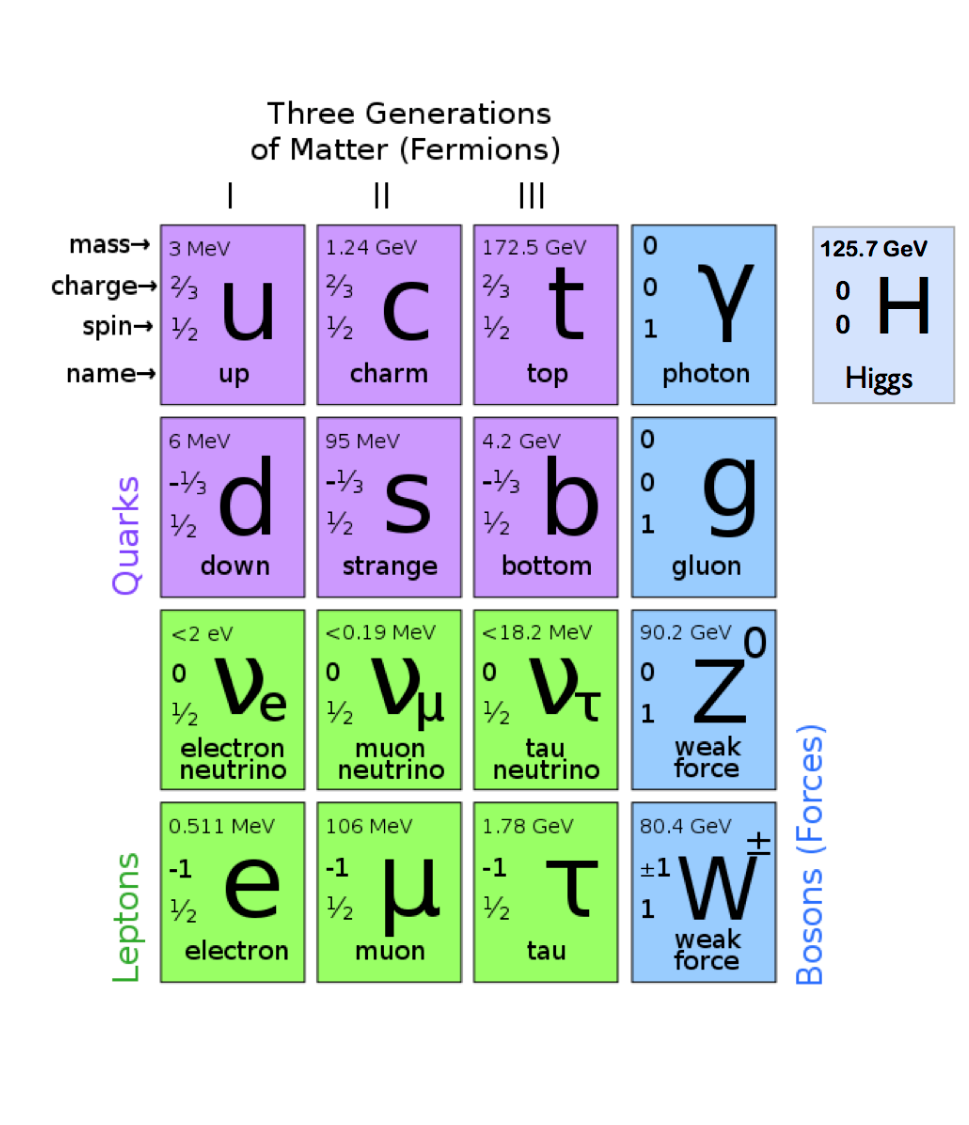
\includegraphics[width=0.7\textwidth]{figures/standard_model.pdf}
\caption[O Modelo Padrão de interação entre as partículas elementares]{
O Modelo Padrão de interação entre partículas elementares. Extraído de
\cite{tese_torres}.}
\label{fig:modelo_padrao}
\end{figure}

\subsection{Os bósons e as interações fundamentais}

As interações são comunicadas através dos bósons, partículas elementares
de campo das interações. Cada interação tem seu bóson característico: o gluôn (g); interação forte; 
o fóton $\gamma$; interação eletromagnética; e os bósons W e Z: interação fraca. Os bósons W e Z 
possuem respectivamente massa de aproximadamente 80 e 90~GeV. Esse fato limita o alcance da 
interação fraca a cerca de $10^{-3}$~fm, uma vez que uma partícula de massa $M$ só pode existir como 
parte de um estado intermediário por tempo $\hbar/Mc^2$, viajando uma distância não maior que
$\hbar/Mc$. O bóson W possui carga elétrica, enquanto o bóson Z é neutro, sendo sua própria 
antipartícula.

O bóson de Higgs (H), previsto inicialmente em 1964 pelo físico britânico Peter Higgs trabalhando
as ideias de Philip Anderson é descrita pelo mecanismo de Higgs sendo está a partícula que dá
massa a todas as outras, inclusive a ela mesma. Até então está partícula não tinha sido observada
devido as limitações tecnológicas da época. Outro problema referente à teoria era que esta não previa a faixa
de energia ou massa em que a partícula poderia ser observada. Porém em 4 de julho de 2012 essa observação
foi anunciada oficialmente em conjunto pelos grupos de físicos dos detectores \gls{atlas} e  \gls{cms}  do 
experimento \gls{lhc} em uma faixa de massa entre 125 e 127 $GeV$.

Por ser uma partícula instável o bóson de Higgs pode decair em $H\to 2Z$ e novamente
em $Z\to e^{+}e^{-}$, onde os elétrons são partículas estáveis e seu comportamento conhecido.
Existem outras formas de decaimento previstos pela teoria que não serão abordados neste
trabalho. Para realizar a observação de Higgs deve-se fazer o caminho inverso da reconstrução, ou seja,
detectar os dois pares de elétrons cujo a massa e outras propriedades físicas formam as
características do bóson Z. Por fim detectar o par intermediário de bósons que juntos reconstroem
as propriedades e massa do bóson H. Por ser o foco deste trabalho, o algoritmo de detecção
desses pares, chamado de   \gls{tap}, será abordado no capítulo seguinte.

Os físicos esperam adicionar a interação gravitacional através da partícula gráviton, que deverá 
ter rotação equivalente a 2 unidades de $\hbar$ e massa nula, entretanto não há nenhuma evidência 
experimental a favor ou contra sua existência \cite{Beiser}.

Os léptons podem ser subdivididos em dois grupos, um com massa e carga elétrica, idêntica e 
unitária: elétron, múon e táu; e outro neutro em carga e massa reduzida, estando relacionados 
com os léptons carregados: neutrino do elétron, neutrino do múon e neutrino do táon. Dos
léptons carregados, o múon e o táu só diferem dos elétrons na sua massa e no seu tempo de vida 
finitos, sendo o elétron o único estável.

Uma dificuldade da investigação experimental dos quarks é devido aos mesmos
nunca terem sido observados isoladamente.  Mesmo em colisões de altas energias os quarks 
se agrupam rapidamente em hádrons, formando jatos hadrônicos \cite{Intro_Nuclear}. Esse 
confinamento dos quarks ocorre porque a interação forte é similar a uma mola, quanto mais 
afastados, maior é a força de atração entre os quarks. Mas se energia suficiente for adicionada,
ao invés de um quark se liberar dos outros no hádron, a energia excedente produz um par de 
quark-antiquark \cite{Beiser}. Se dá ao nome dos sistemas compostos por quarks e gluôns de
hádrons, sendo os bárions e mésons os sistemas mais simples conhecidos. 

Um largo espectro dos bárions pode ser explicado como uma cápsula contendo
três quarks confinados por gluôns, sendo exemplos os prótons e nêutrons. Os mésons
são compostos essencialmente por um quark e antiquark ligados transitivamente por um gluôns. 
O próton é o único bárion estável\footnote{Teorias atuais
consideram que o próton decai com um tempo de vida muito longo, entretanto esse valor talvez seja 
maior que o valor mínimo detectado experimentalmente, de $10^{32}$~anos.  Para comparação, a 
idade do universo é de $10^{10}$~anos \cite{Beiser}.}, já o nêutron ($udd$), apesar de estável 
na estrutura atômica, quando isolado tem vida média de 15~minutos~\cite{Intro_Standard}. Finalmente, 
todos os mésons são instáveis e também são bósons, uma vez que mediam a interação
forte entre hádrons.

\section{O \emph{Large Hadron Collider} (LHC)}

O LHC começou a ser construído em 1998 com a colaboração de mais de 100 países, conta com um 
túnel de 27 km de circunferência, ao custo de aproximadamente  \euro $7,5 Bi$. Está em funcionando 
desde 10 de Setembro de 2008, tendo ocorrida sua primeira colisão entre prótons um ano e meio depois. Após as 
colisões entre 2010 e 2012, chamada de $run 1$, o \gls{lhc} passou por uma fase de $upgrade$
que perdurou até meados de 2015 quando foi finalmente religado. Para essa nova fase do calendário previsto
pela colaboração, chamado de $run 2$, espera-se colisões utilizando a energia nominal de 14TeV para
colisões de prótons.

\begin{figure}[h!t]
\centering
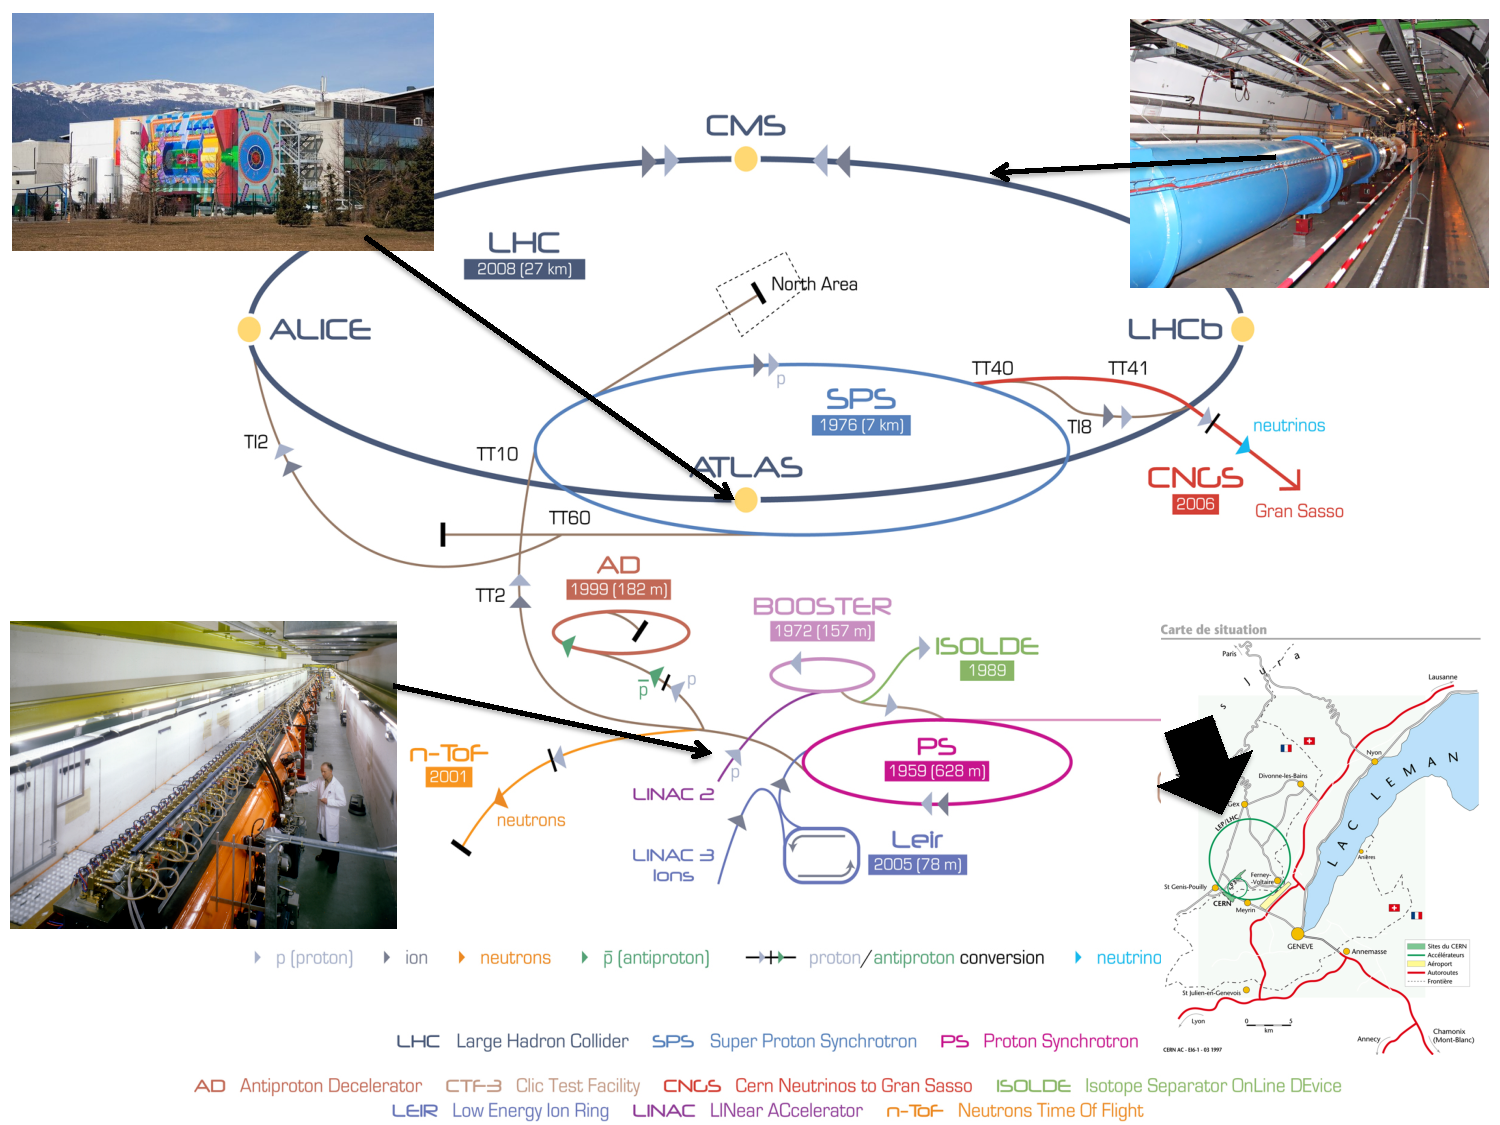
\includegraphics[width=\textwidth]{figures/lhc-overview.pdf}
\caption[A cadeia de aceleração do LHC]{
Os diferentes aceleradores da cadeia e detectores do CERN, extraído de
\cite{cern_accelerators}. A seta cinza claro corresponde ao sentido do
deslocamento de prótons nos aceleradores, No canto superior esquerdo
a foto do centro de controle do detector \gls{atlas}. No canto inferior esquerdo, a
foto do acelerador LINAC 2. No canto superior direito, a foto de uma seção do \gls{lhc}.
No canto inferior direito o mapa que mostra a localização do  \gls{lhc} na fronteira entre
a França e a Suíça.}
\label{fig:esquema_aceleradores}
\end{figure}

Para desenvolver a altíssima energia necessária para o experimento, o \gls{cern}
utiliza outros aceleradores construídos anteriormente, acelerando sequencialmente os pacotes 
de prótons até atenderem a energia desejada para a colisão. Na Figura \ref{fig:esquema_aceleradores} 
pode-se observar o esquema de aceleração, tanto para prótons, quanto para íons de chumbo. 
No caso dos prótons, o ciclo inicia-se na extração de prótons de átomos de hidrogênio que são
acelerados no \acrshort{linac} 2, um acelerador linear, que inicia a sequencia de aceleração, 
proporcionando-lhes uma energia de até 50 MeV.  Em seguida são utilizados síncrotrons, aceleradores 
circulares no qual as partículas seguem trajetórias circulares dirigidas por magnetos: \acrshort{booster} (1,4~GeV), 
\acrshort{psync} (25~GeV), \acrshort{sps} (450~GeV), até finalmente abastecer o \gls{lhc} com os pacotes 
de prótons. O \gls{lhc} também é um síncrotron, assim como grande parte dos aceleradores de altas 
energias anteriormente construídos \cite{lecture_slides_1,lecture_slides_2}.

Uma vez atingida a energia desejada para as colisões dos hádrons no \gls{lhc}, os pacotes serão então 
colididos nos \glspl{ip} experimentais. Esses pontos de colisão são formados pelos quatro principais detectores específicos 
para cada experimento. Os detectores \gls{atlas} e o \gls{cms} são utilizados para o estudo geral da matéria, o \gls{alice} 
é especializado em descobrir o mistério da matéria quente e densa que é brevemente criada quando da colisão de ions 
pesados a altas energias. Por fim, o \gls{lhcb} é um experimento desenvolvido para medidas precisas da violação da simetria 
e decaimentos raros de mésons com o quark b ou anti-b. A Figura ~\ref{fig:detectores} mostra uma visão global da 
arquitetura de cada um dos quatro principais detectores instalados no complexo. 

\begin{figure}[h!t]
\centering
\includegraphics[width=1\textwidth]{figures/detectors.pdf}
\caption[Os detectores do LHC.]{
Os quatro principais detectores instalados no complexo do \gls{lhc}. No canto superior esquerdo, o detector 
 \gls{atlas}. No canto superior direito, o detector \gls{alice}. No inferior direito, o \gls{lhcb} e, finalmente, no
 canto inferior esquerdo, o detector \gls{cms}.}
\label{fig:detectores}
\end{figure}

\newpage

\section{A Cinemática das Colisões}
\label{sssec:cinematica}

Ainda que não seja o objetivo do trabalho, um breve resumo da cinemática
relativística envolvida nas interações de partículas ajudará a entender algumas
das variáveis comumente utilizadas. 
Como o trabalho está englobado no experimento \gls{atlas}, irá se considerar o 
eixo de coordenadas adotado para o \gls{ip}1, ponto de inserção do mesmo. 

Normalmente se utilizam coordenadas esféricas ($p,\theta,\phi$), uma vez que 
essa é a geometria das colisões.
Seus eixos definidos em coordenadas retangulares estão dispostos 
na Figura~\ref{fig:atlas_p1_coord}, sendo o eixo \emph{z} a direção do feixe com
o lado positivo na direção do \gls{ip}8, o eixo
\emph{x} aponta na direção do centro do anel do \gls{lhc} e o eixo \emph{y}
aponta para a superfície.  
As transformações para coordenadas cilíndricas
são bem conhecidas e realizadas através da equação \ref{eq:transf_cil}.  
A física é simétrica em relação ao \gls{phi}, 
mas há correlação entre o
tipo de colisão com o \gls{theta}, onde geralmente quanto mais intensa a
interação ocorrida durante a colisão mais próximo de $90^\circ$ será esse
ângulo. O plano transverso é definido 
pelo corte transversal à direção de propagação do feixe, sendo o plano-xy do
sistema de coordenadas descrito, e a componente restante, paralela a direção de
propagação do feixe ($z$), é chamada de componente longitudinal.

\begin{figure}[h!t]
\centering
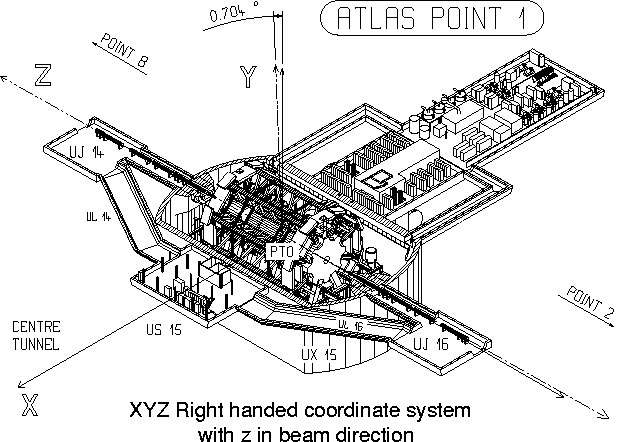
\includegraphics[width=0.7\textwidth]{figures/atlas_p1_coord.png}
\caption[O Sistema de Coordenadas adotado para o ATLAS]{O Sistema de Coordenadas adotado para o IP1, ponto de inserção do
experimento ATLAS. Extraído de \cite{tese_torres}.}
\label{fig:atlas_p1_coord}
\end{figure}

\begin{subequations}\label{eq:transf_cil}
\begin{equation}\label{eq:transf_phi}
\phi = arctan\left( \frac{x}{y} \right) \\
\end{equation}
\begin{equation}\label{eq:transf_theta}
\theta = arctan\left( \frac{x}{z} \right) 
\end{equation}
\end{subequations}

Estando interessado no momento das partículas
produzidas, a fim de se evitar as transformações de Lorentz, se faz mão de dois
parâmetros. Um deles, a \gls{y}, foi introduzido pela métrica de Minkowski
\cite{schlippe} e está definido na equação~\ref{eq:rapidez}.
O outro é o \gls{pt}, a projeção do momento no plano
transverso, dado pela Equação ~\ref{eq:pt}. 
Esses parâmetros são invariantes as transformações relativísticas 
longitudinais. O \gls{pl}, que não é conservado nas colisões entre hádrons por
esses não serem partículas ponto, pode ser obtido através
da Equação~\ref{eq:pl}. Outras duas variáveis que também
são projetadas no plano transverso são a \gls{mt} e \gls{Et}, obtidas através das
relações~\ref{eq:mt} e \ref{eq:Et}. Uma relação muito importante é a relação
massa-momento, dada pela equação~\ref{eq:rel_mom}.

\begin{equation}\label{eq:rapidez}
y = \frac{1}{2}ln\left(\frac{E+p_z}{E-p_z}\right)
\end{equation}

\begin{equation}\label{eq:rel_mom}
m^2c^4 = E^2 - p^2c^2
\end{equation}

\begin{subequations}\label{eq:proj_transv}
\begin{equation}\label{eq:pt}
p_T = p sen ( \theta ) = \sqrt{(p_x^2 + p_y^2)}
\end{equation}
\begin{equation}\label{eq:mt}
m_T = m^2 + p_T
\end{equation}
\begin{equation}\label{eq:Et}
E_T = E sen ( \theta )
\end{equation}
\end{subequations}

\begin{equation}\label{eq:pl}
p_L = p_z = m_T senh ( y )
\end{equation}

Os detectores absorvem a energia total (E) de grande parte das partículas
geradas nas colisões através de seus calorímetros, 
estando a mesma relacionada com a \gls{mt} por \ref{eq:etot}. Entretanto, na física de 
altas energias algumas aproximações podem
ser feitas de modo a facilitar a manipulação dos parâmetros. No caso ultrarrelativístico (quando $p \gg
m$) a rapidez se aproxima da \gls{eta}, parâmetro relacionado a \gls{theta}
através das equações \ref{eq:eta} \cite{pdg_book}.
Ainda, nesses casos a \gls{mt} tende a se aproximar de
\gls{pt}, e a energia total das partículas é predominantemente dado
pelo momento das partículas. Dessa forma, ao se projetar a energia absorvida
pelo calorímetro no plano transverso obtêm-se diretamente o \gls{pt} das
partículas, Equação~\ref{eq:e_pt}, obtida aplicando as relações \ref{eq:eta} em \ref{eq:etot}.

\begin{equation}\label{eq:etot}
E = m_{T}cosh(y) \approx m_{T}cosh(\eta) \approx p_{T}cosh(\eta)
\end{equation}
\begin{equation}\label{eq:eta}
\eta = -ln \left( tan\left( \frac{\theta}{2} \right) \right) \;,\; senh(\eta) =
cot(\theta) \;,\;  cosh(\eta) = 1 / sen(\theta) \;,\; tanh(\eta) = cos(\theta) 
\end{equation}
\begin{equation}\label{eq:e_pt}
p_T \approx \frac{E}{sen(\theta)}
\end{equation}



\section{O Detector de Partículas ATLAS}

\glsreset{atlas}
O ATLAS \cite{ATLAS_TDR,ATLAS_TDR2,paper_atlas}, Figura~\ref{fig:det_atlas}, é o maior 
dos detectores que operam no \gls{lhc}, medindo 45~metros de comprimento e 25~metros de altura 
e largura. Ele é um detector de propósito geral, registrando dados sobre os eventos de colisões de 
partículas que podem ser usados para estudos em diversas áreas da física. Cada uma de suas partes 
teve seus componentes construídos por um grupo diferente pertencente às instituições colaboradoras. 
Sua colaboração internacional envolve cerca de 2500 físicos de mais de 174 instituições 
e laboratórios de 38 países \cite{webATLAS}. Esses números incluem a \acrshort{ufrj}, que participa 
através da \acrshort{coppe}, da Escola Politécnica e do Instituto de Física. 

\begin{figure}[h!t]
\centering
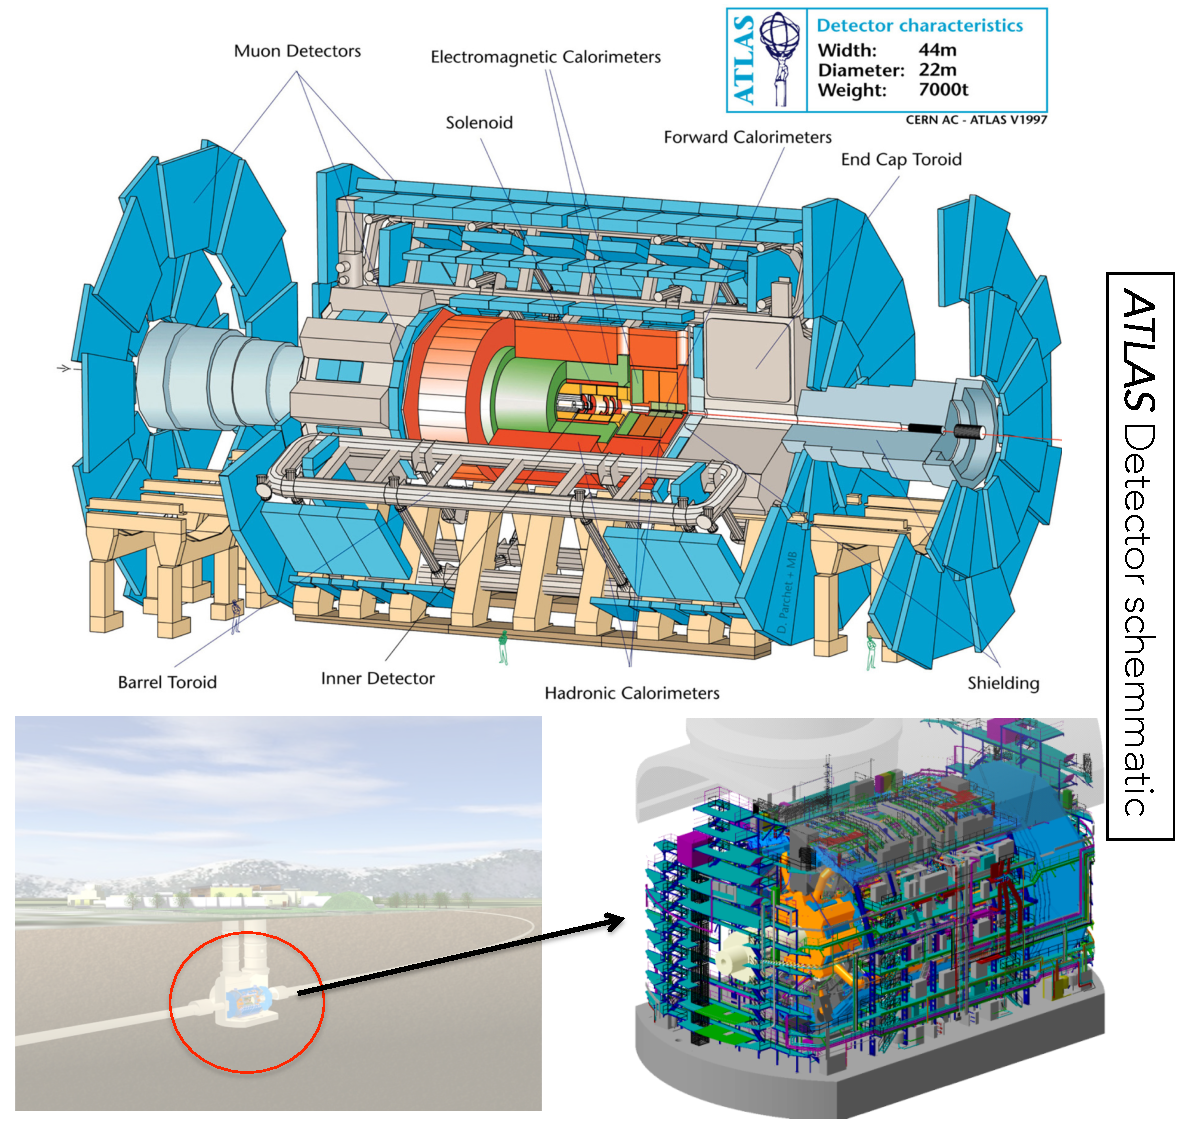
\includegraphics[width=1.1\textwidth]{figures/atlas-detector-overview.pdf}
\caption[O detector ATLAS.]{
O detector \gls{atlas} em diferentes níveis de detalhe. A ilustação do canto inferior esquerdo representa
a visão subterrânea da caverna onde está instalado o detector. O esquemático no canto direito representa
em detalhes a estrutura em volta do detector. A ilustração superior representa uma visão do detector em
cortes. Desde a parte mais interna, começando com o \gls{id}, até a camada mais externa dos subdetectores
de múons instalados em volta dos calorímetros.}
\label{fig:det_atlas}
\end{figure}


O \gls{atlas} possui 4 subdetectores, com um total de $~140$~M de canais de
leitura, sendo do mais interno para o mais externo:  \gls{id}\footnote{O \gls{id} 
também é referido como Detector de Traços.}, \gls{ecal}, \gls{hcal} e Espectrômetro 
de Múons. De maneira resumida, o \gls{id} identifica a trajetória e o momento de 
partículas carregadas, os calorímetros fazem a absorção das partículas medindo 
assim sua energia total, e o Espectrômetro de Múons é responsável exclusivamente 
pela detecção de múons. Através das assinaturas feitas pelas partículas nesses 
subdetectores é possível realizar a identificação das mesmas. A Figura~\ref{fig:particulas_atlas} 
contém um esboço de como as diferentes partículas idealmente interagem com os 
subdetectores do \gls{atlas}. 

Nas próximas subseções serão descritos em detalhes cada um dos sistemas instalados no detector, em especial 
o calorímetro eletromagnético e hadrônico responsáveis por absorver elétrons, fótons e partículas hadrônicas,
sendo estas as principais partículas a serem discriminadas pelo sistema proposto por este trabalho.

\begin{figure}[h!t]
\centering
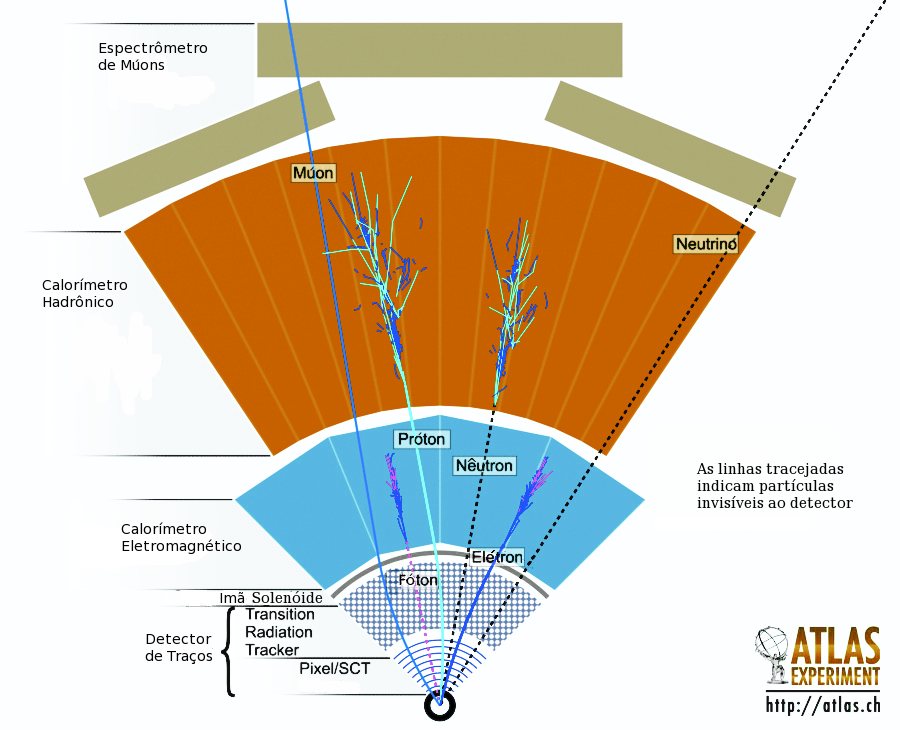
\includegraphics[width=0.8\textwidth]{figures/particulas_subdetectores_3.png}
\caption[Esboço contendo exemplos de interação de partículas com os
subdetectores do ATLAS]
{Um esboço contendo exemplos de interação de partículas com os
subdetectores do ATLAS. 
Apenas partículas carregadas eletricamente deixam traços no Detector Interno. 
Elétrons, pósitrons e fótons serão totalmente absorvidos pelo Calorímetro 
Eletromagnético. Ao Calorímetro Hadrônico, cabe a tarefa de absorver 
partículas com componentes hadrônicas, como nêutrons, prótons e outros mésons. Múons
mesmo contendo componentes eletromagnéticas devem atravessar os calorímetros com
facilidade, sendo somente detectados pelo Espectrômetro de Múons. Léptons Neutrinos não
são detectados por nenhum dos subdetectores do ATLAS. Adaptado de \cite{particulas_atlas}.}
\label{fig:particulas_atlas}
\end{figure}

\newpage

\glsreset{id}

\subsection{O Detector Interno}
\label{ssec:det_int}

O \gls{id} \cite{inner_tdr1,inner_tdr2}, Figura~\ref{fig:det_interno}, é o responsável pela identificação das 
trajetórias de partículas carregadas, medir o seu momento, o
vértice primário\footnote{local aonde ocorreu a colisão dos hádrons no detector}, os
vértices de decaimentos de partículas e a distância entre o vértice primário e o ponto mais próximo do traço
\cite{tese_jatos,ATLAS_TDR}. Ele cobre uma região com completa cobertura em
\gls{phi} de maneira simétrica para $|\gls{eta}| < 2,5$, a chamada região de precisão
do detector.  


A medição do momento é realizada através da deflação das partículas pelo
\gls{campmag} e sua resolução depende da \gls{respos}, da magnitude de
\gls{campmag} e do \gls{comprimento} do rastreador de acordo com a Equação \ref{eq:res_mom}
\cite{lecture_slides_1,lecture_slides_2}. O \gls{campmag} é fornecido pelo
\gls{cs} restando apenas dois parâmetros a serem explorados, o \gls{respos} e \gls{comprimento}. 
A resolução de vértices é proporcional a capacidade de reconstrução da trajetória da partícula e 
assim como o momento é inversamente proporcional à posição \gls{respos}. 

Também é necessário uma baixa granularidade, devido há uma grande densidade de
traços gerados no \gls{lhc} resultando em $\approx$10.000 traços no intervalo de 
100~$n$s~\cite{resumo_ATLAS}, e à baixa quantidades de material no \gls{id} 
para que seja possível realizar medições nos calorímetros sem que as partículas 
interajam e percam energia nos componentes deste detector.

\begin{equation}\label{eq:res_mom}
\frac{\delta p_T}{p_T} = \frac{p_T \sigma_p}{0,3Bl^2} [GeV,T,m]
\end{equation}

\begin{figure}[h!t]
    \label{fig:det_interno}
    \begin{center}
        \subfigure[Seção de corte do Detector Interno mostrando seus subsistemas. Extraído de
\cite{paper_atlas}.  ]{%
            \label{fig:id_secao}
            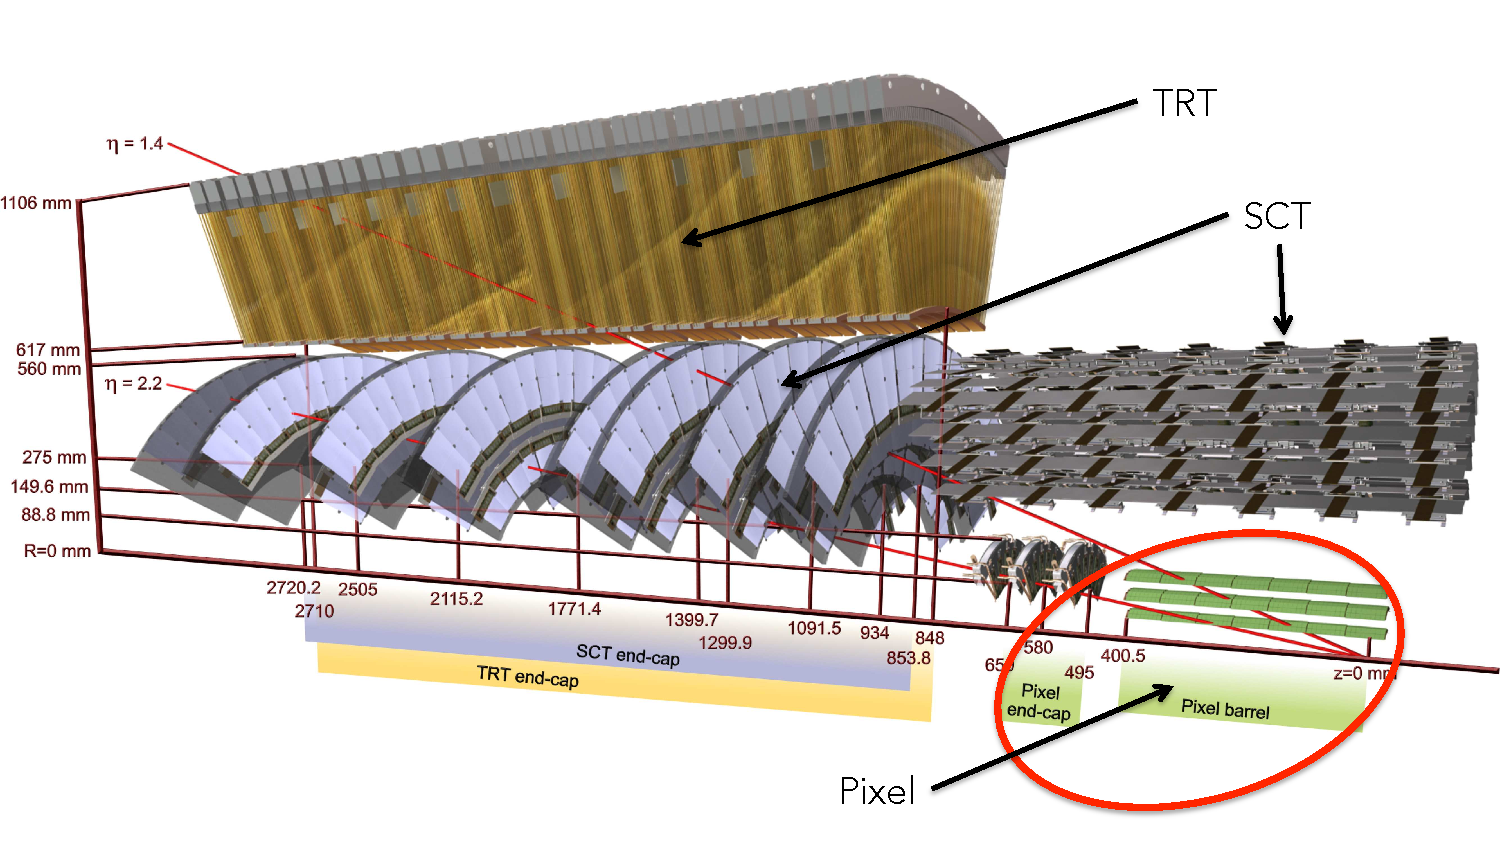
\includegraphics[width=\textwidth]{figures/id_lateral_2.pdf}
        }\\
        \subfigure[Esboço do Detector Interno, contendo suas dimensões e
pseudorrapidez relacionas. Extraído de \cite{paper_atlas}.]{%
            \label{fig:id_eta}
            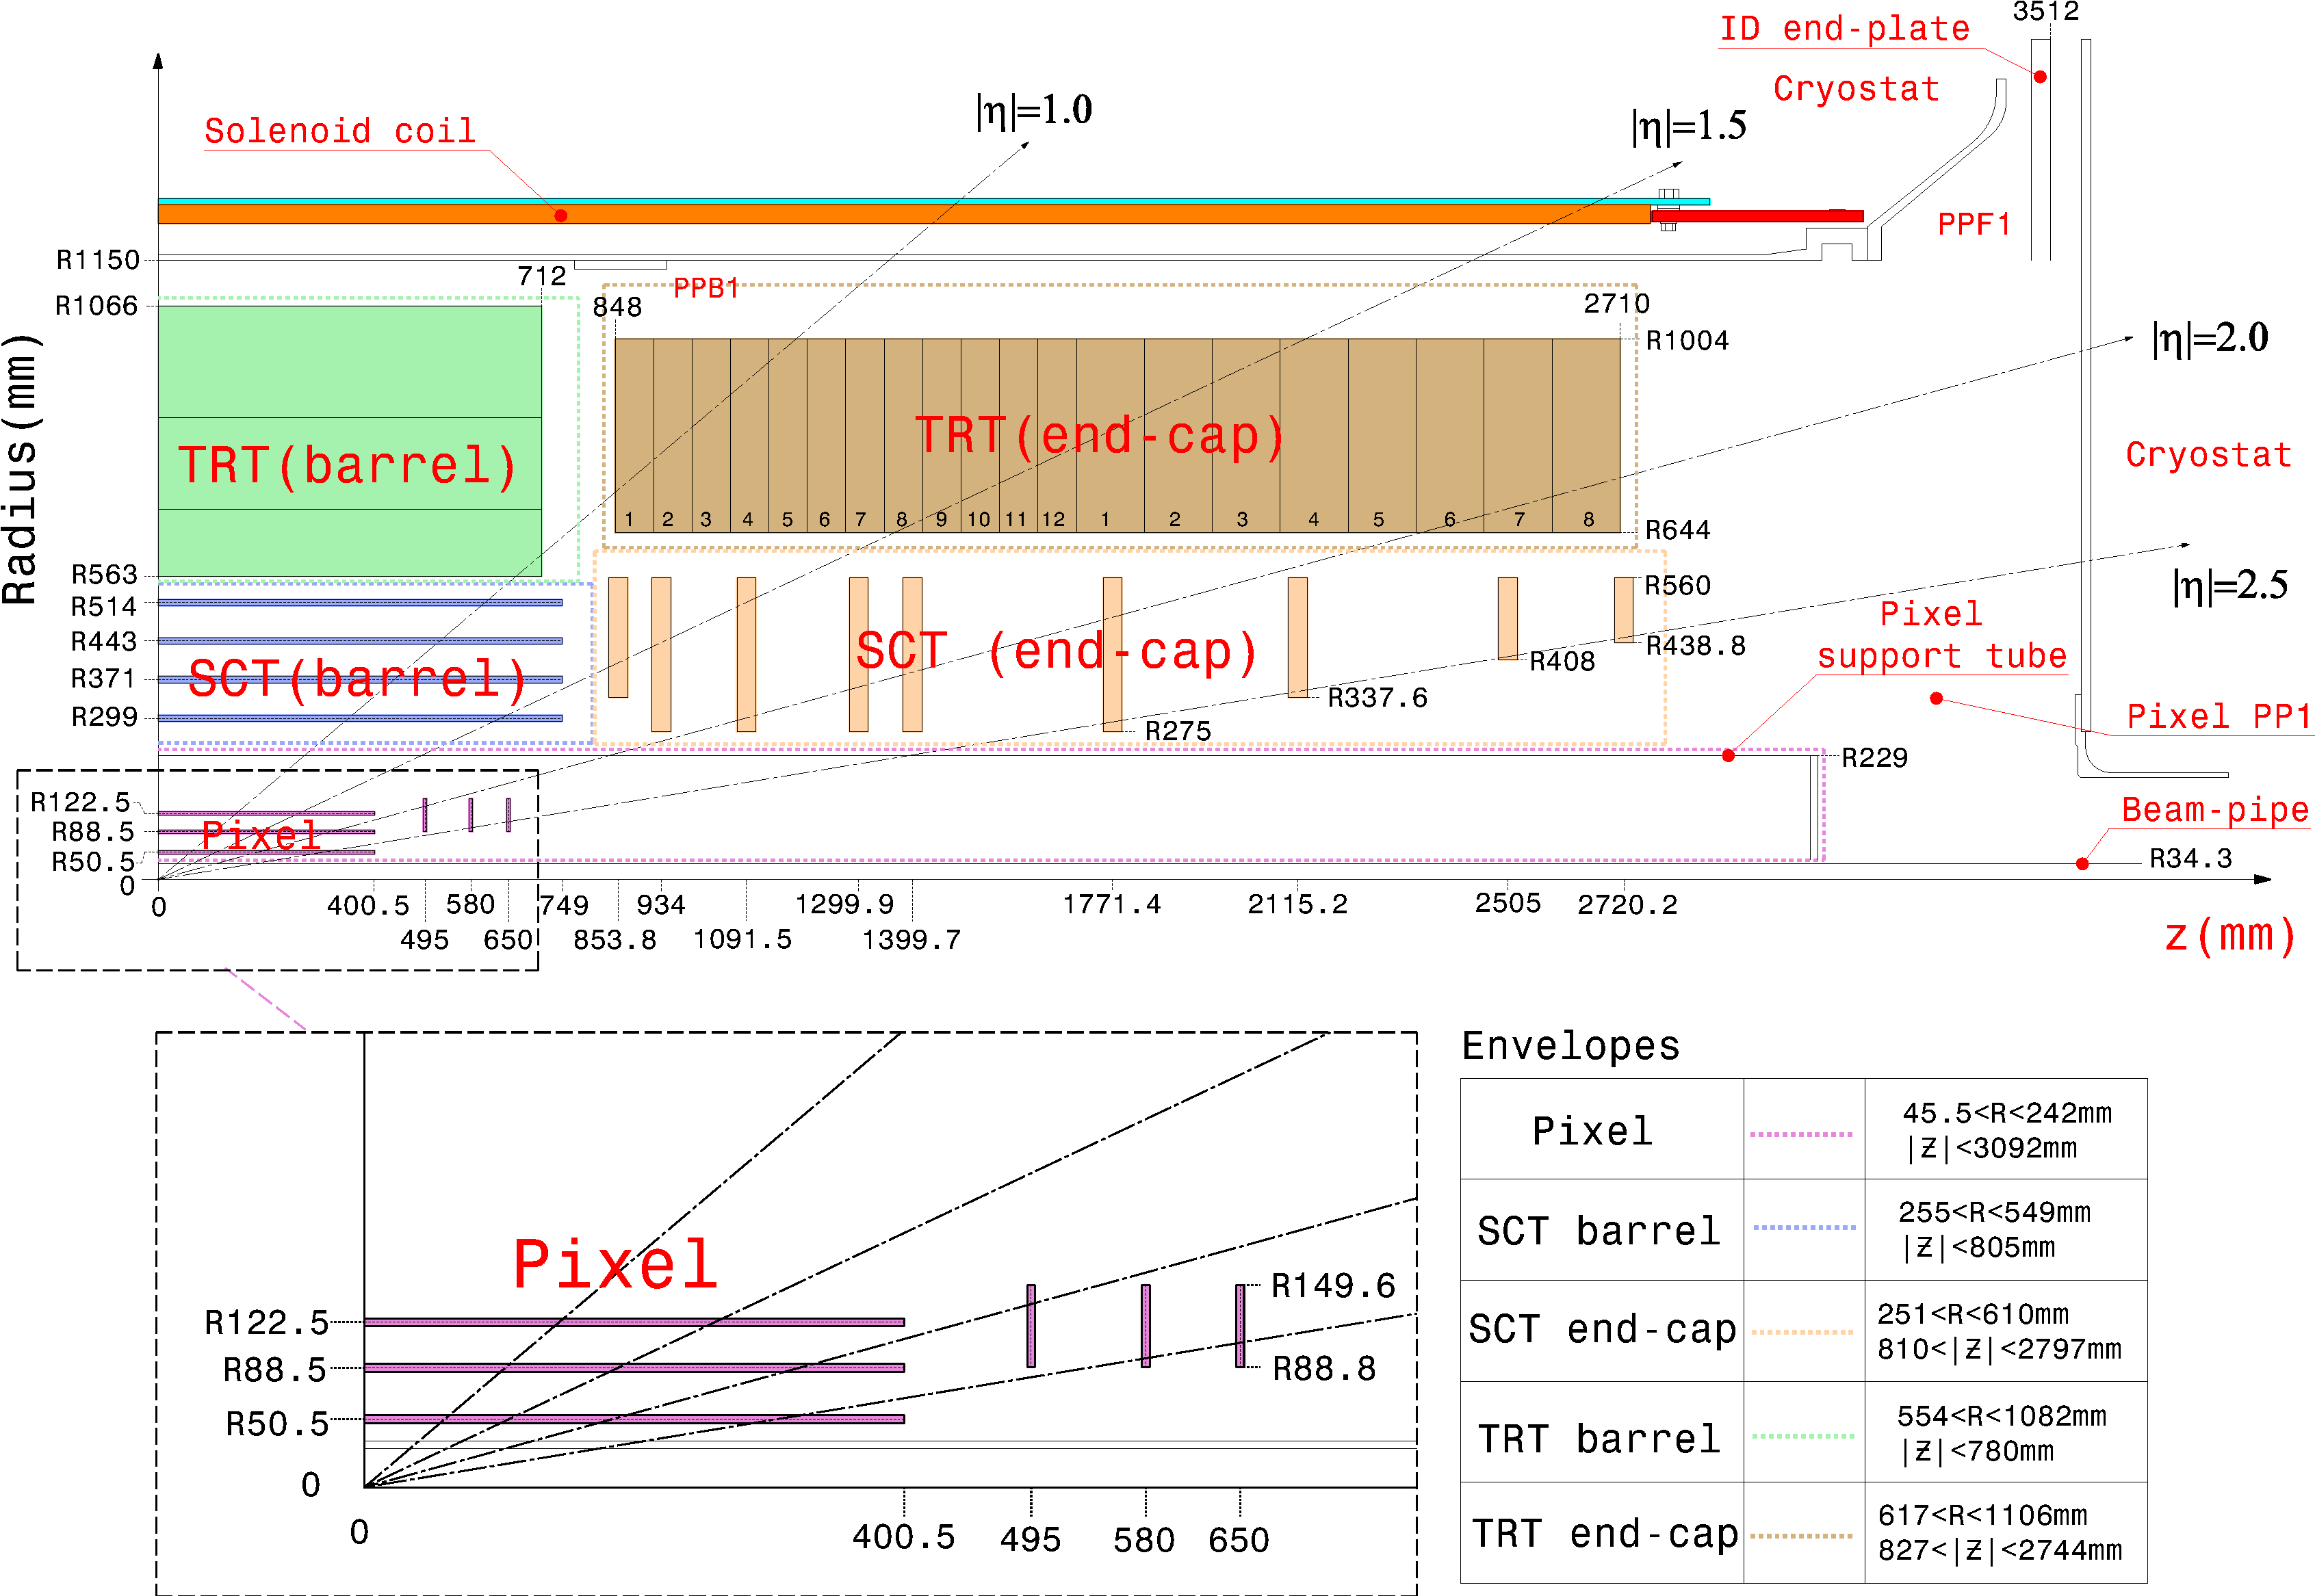
\includegraphics[width=.8\textwidth]{figures/id_eta.pdf}
        }
    \end{center}
    \caption[O Detector Interno (ID)]{O Detector Interno.}%
\end{figure}

O \gls{id} dispõe de dois medidores de alta precisão, que exploram a redução 
de \gls{respos} para melhorar a resolução do detector. Os detectores de alta 
precisão são formados pelos Detectores de Pixel e \gls{sct}. O \gls{trt}
explora o acréscimo do \gls{comprimento} do detector em busca de uma melhor
resolução de momento. Um resumo das capacidades de
cada um dos detectores é fornecido na Tabela~\ref{tab:info_id}.

\begin{table}
\centering
\resizebox{\textwidth}{!}{
\begin{tabular}{lp{5cm}cccp{2cm}}
\hline
\hline
\textbf{Sistema} & \textbf{Posição} & \textbf{Área} ($\text{m}^2$) & \textbf{\gls{respos}
($\mu$m)} & \textbf{Canais ($10^6$)} & \textbf{Cobertura em $|\eta|$} \\
\hline
\hline
Pixeis & 1 camada removível no barril (Camada B) & 0,2 & R$\phi$ = 12, z = 66 & 16
& $\leq 2,5$ \\
& 2 camadas no barril & 1,4 & R$\phi$ = 12, z = 66 & 81 
& $\leq 1,7$ \\
& 3 discos nas tampas de cada lado & 0,7 & R$\phi$ = 12, R = 77 & 43 
& $1,7-2,5$ \\
\hline
SCT & 4 camadas no barril & 34,4 & R$\phi$ = 16, z = 580 & 3,2
& $\leq 1,4$ \\
& 9 discos nas tampas de cada lado & 26,7 & R$\phi$ = 16, R = 580 & 3,0
& $1,4-2,5$ \\
\hline
TRT & Canudos axiais no barril &  & 170 (por canudo) & 0,1
& $\leq 0,7$ \\
& Canudos radiais nas tampas &  & 170 (por canudo) & 0,32
& $0,7-2,5$\\
\hline
\hline
\end{tabular}
}
\caption[Parâmetros do ID]
{Parâmetros do ID. As resoluções estão citadas em valores típicos (a
resolução verdadeira em cada detector depende do ângulo de impacto). Adaptado de
\cite{ATLAS_TDR}.}
\label{tab:info_id}
\end{table}



\subsubsection{Detector de Pixeis}
\label{sssec:pixeis}

A maior granularidade é atingida pelos pixels semicondutores próximos
ao vértice da colisão, entretanto o número de camadas de precisão devem ser
limitadas devido à grande quantidade de material introduzida e ao seu alto
custo. Dessa forma, o Detector de Pixel utilizado foi projetado para
fornecer apenas três pontos de alta precisão. Ele determina a resolução do
\gls{d0} e a habilidade do \gls{id} de encontrar partículas de curta
vida como hádrons B e táons. Um total de 140~M de canais de
leitura estão dispostos com um afastamento de 50~$\mu$m na direção R$\phi$, 
mesma direção que o plano transverso, e 300 $\mu$m em z. 
O sistema consiste de três barris a uma distância radial
média de $\sim$5~cm, 10~cm, 13~cm, e três tampas em cada lado entre uma distância 
radial de 11 e 20~cm.

\subsubsection{Detector de Rastreamento por Semicondutores (SCT)}
\label{sssec:sct}

O \gls{sct} foi projetado para fornecer oito pontos de precisão por traço na
região intermediária do \gls{id}, contribuindo tanto para a medição do momento,
parâmetro de impacto e posição do vértice primário, quanto provendo bom
reconhecimento de padrões pelo uso de alta granularidade. O seu barril usa oito
camadas de microfibras de silicone para gerar precisão nos pontos nas
coordenadas de R$\phi$ e z. Cada componente mede $6,36\times6,40 \text{cm}^2$ com 768 canais de
leitura com 80~$\mu$m de afastamento. A tampa possui construção similar, mas usa
tiras cilíndricas, formando um conjunto alinhado radialmente. Ela possui cerca de 61~$m^2$ 
de detectores de silicone, com 6,2~M de canais, que permitem distinguir
dois traços separados por cerca de $\sim200~\mu$m.

\subsubsection{Detector de Rastreamento por Transição de Radiação (TRT)}
\label{sssec:trt}

Por outro lado, o \gls{trt} explora a medição contínua do traço com uma
quantidade bem menor de material e custo. Ele fornece cerca de 36 pontos por
traço, melhorando assim a resolução do momento ao explorar um maior
\gls{comprimento}. Ele se baseia em detectores de canudos, que podem operar nas
grandes taxas esperadas no \gls{lhc} em virtude de seus pequenos diâmetros e
isolamento dos sensores dentro de volumes individuais de gás. A capacidade de
identificação de elétrons é adicionada aplicando xenônio para detectar fótons de
radiação transiente em seu radiador entre os canudos. O barril contém cerca de
50.000~canudos, divididos em dois no seu centro para reduzir a ocupação, e sua
leitura em cada ponta. A tampa contém~320.000 canudos radiais, com a leitura na
ponta externa. As medições realizadas pelos canais são em formas de
impulsos e dão uma resolução espacial de 170~$\mu$m por canudo.


%----------------------------- CALORIMETRIA --------------------------------
\newpage
\subsection{O Sistema de Calorimetria}
\label{ssec:calorimetria}

Na calorimetria \cite{wigmans,tese_torres}, a energia das partículas é 
absorvida através de suas interações com o calorímetro, sendo assim um processo 
de detecção destrutivo, ou seja, não é possível realizá-lo novamente. Os calorímetros 
podem ser de dois tipos: homogêneos ou de amostragem. 

O método de amostragem utiliza-se de dois materiais: o material passivo 
responsável pela interação com a partícula, realizando a absorção de energia da
partícula; e o ativo, no qual ocorre a geração, ou amostragem, do sinal. 
Calorímetros homogêneos utilizam um único material para realizar as duas
tarefas: a de interagir com a partícula e gerar sinal; e por isso apresentam melhor resolução de energia 
que os de amostragem, uma vez que parte da energia das partículas nas interações com o
material passivo dos calorímetros de amostragem é perdida. Por sua vez, calorímetros de amostragem são
mais baratos e por isso utilizados em sistemas de detecção muito grandes, como o
\gls{atlas}. Além disso, a resolução de energia do calorímetro para o método de 
amostragem melhora para partículas de maior energia.

Uma partícula, ao transpassar o material do calorímetro geralmente interage de
forma a excitar o meio ou aquecê-lo. O tipo de interação ocorrida depende da
quantidade de energia da partícula, de sua natureza, assim como do
meio, podendo ter como resultado interações eletromagnéticas, fortes, e mais 
raramente, fracas. Em altas energias os processos de interação com o meio 
criam uma cadeia contínua de eventos, provocando os chamados chuveiros de partículas. 


\subsubsection{Utilização dos calorímetros para identificação de partículas}
\label{par:cal_part_id}

\glsreset{ecal}
\glsreset{hcal}

Sabendo como as partículas hadrônicas e eletromagnéticas reagem com
o calorímetro, cabe fazer algumas considerações sobre os calorímetros
responsáveis pela detecção das mesmas. 

O \gls{ecal} é responsável pela absorção de partículas puramente \gls{em}, ou seja, que não têm componentes
\gls{had}, como os léptons carregados e fótons. Os múons, embora façam parte do
grupo de partículas puramente \gls{em}, atravessam
grandes quantidades de material perdendo pouca energia uma vez que são bem mais
maciços que elétrons e por isso é utilizado o Espectrômetro de Múons para
detectá-los. Táons são ainda mais maciços e precisariam de mais
material que os múons para serem detectados. Entretanto, eles tem tempo de vida muito curto e
decaem em múons (ou elétrons) e mais dois neutrinos antes de atingirem o detector, sendo detectados
indiretamente através dos resíduos de seu decaimento. Com isso, apenas elétrons,
pósitrons e fótons são detectados no \gls{ecal}, mas vale ter em mente que eles
podem ser estados finais de outras partículas. 

Por outro lado, o \gls{hcal} deve absorver todas as partículas \gls{had}, como os jatos
\gls{had} que podem ser resíduos de um \gls{ue} e \gls{mbias}, ou até mesmo de
um decaimento. Alguns canais de interesse desejam encontrar jatos, como 
o decaimento do bóson W em altos \gls{pt} para $|\gls{eta}|<3$: $W\rightarrow jato-jato$. 
Entretanto, é necessário separar esses jatos dos criados pelo ruído 
gerados por \gls{mbias} e \glspl{ue}, e para isso o \gls{hcal} deve ser capaz de
separar um jato de um decaimento duplo em jatos próximos, sendo
necessário uma granularidade maior nessa região.

Quanto maior o número atômico do meio, maior será a profundidade no qual um
chuveiro \gls{had} irá se propagar no mesmo, quando em comparação com um chuveiro
\gls{em} de mesma energia. Isso culmina na disposição
dos \gls{ecal} serem anteriores ao dos \gls{hcal}, uma vez que é inútil, assim, utilizar calorímetros com a 
configuração espacial oposta, já que todos os chuveiros de partículas se
extinguiriam no \gls{hcal}, não atingindo o \gls{ecal}. Ainda, é interessante a
utilização de materiais com grandes números atômicos no \gls{ecal} para
garantir, por esse motivo, a menor deposição de energia possível de partículas
\gls{had} no mesmo.

Ainda, o perfil de chuveiros \gls{had} é mais largo que o de chuveiros
\gls{em}. Essa ocorrência é muito explorada para realizar a discriminação 
entre as partículas que interagem com os calorímetros, buscando perfis de chuveiros
justos para partículas \gls{em}. Ela tem como consequência 
a menor granularidade no \gls{ecal} quando comparados com os \gls{hcal}, já que
para realizar a discriminação é necessário que o calorímetro tenha resolução
para discernir entre os chuveiros. Ao mesmo tempo, se faz desnecessário
utilizar altas granularidades no \gls{hcal}, justamente pelos chuveiros se
espalharem por uma região maior.


\subsubsection{Os subsistemas de calorimetria e suas topologias}
\label{sssec:cal_estrutura}

O Sistema de Calorimetria \cite{cal_tdr,ecal_tdr,hcal_tdr} do \gls{atlas}, retratado na
Figura~\ref{fig:cal_atlas}, consistem de calorímetros de amostragem com 
simetria e cobertura total em \gls{phi}.

\begin{figure}[h!t]
\centering
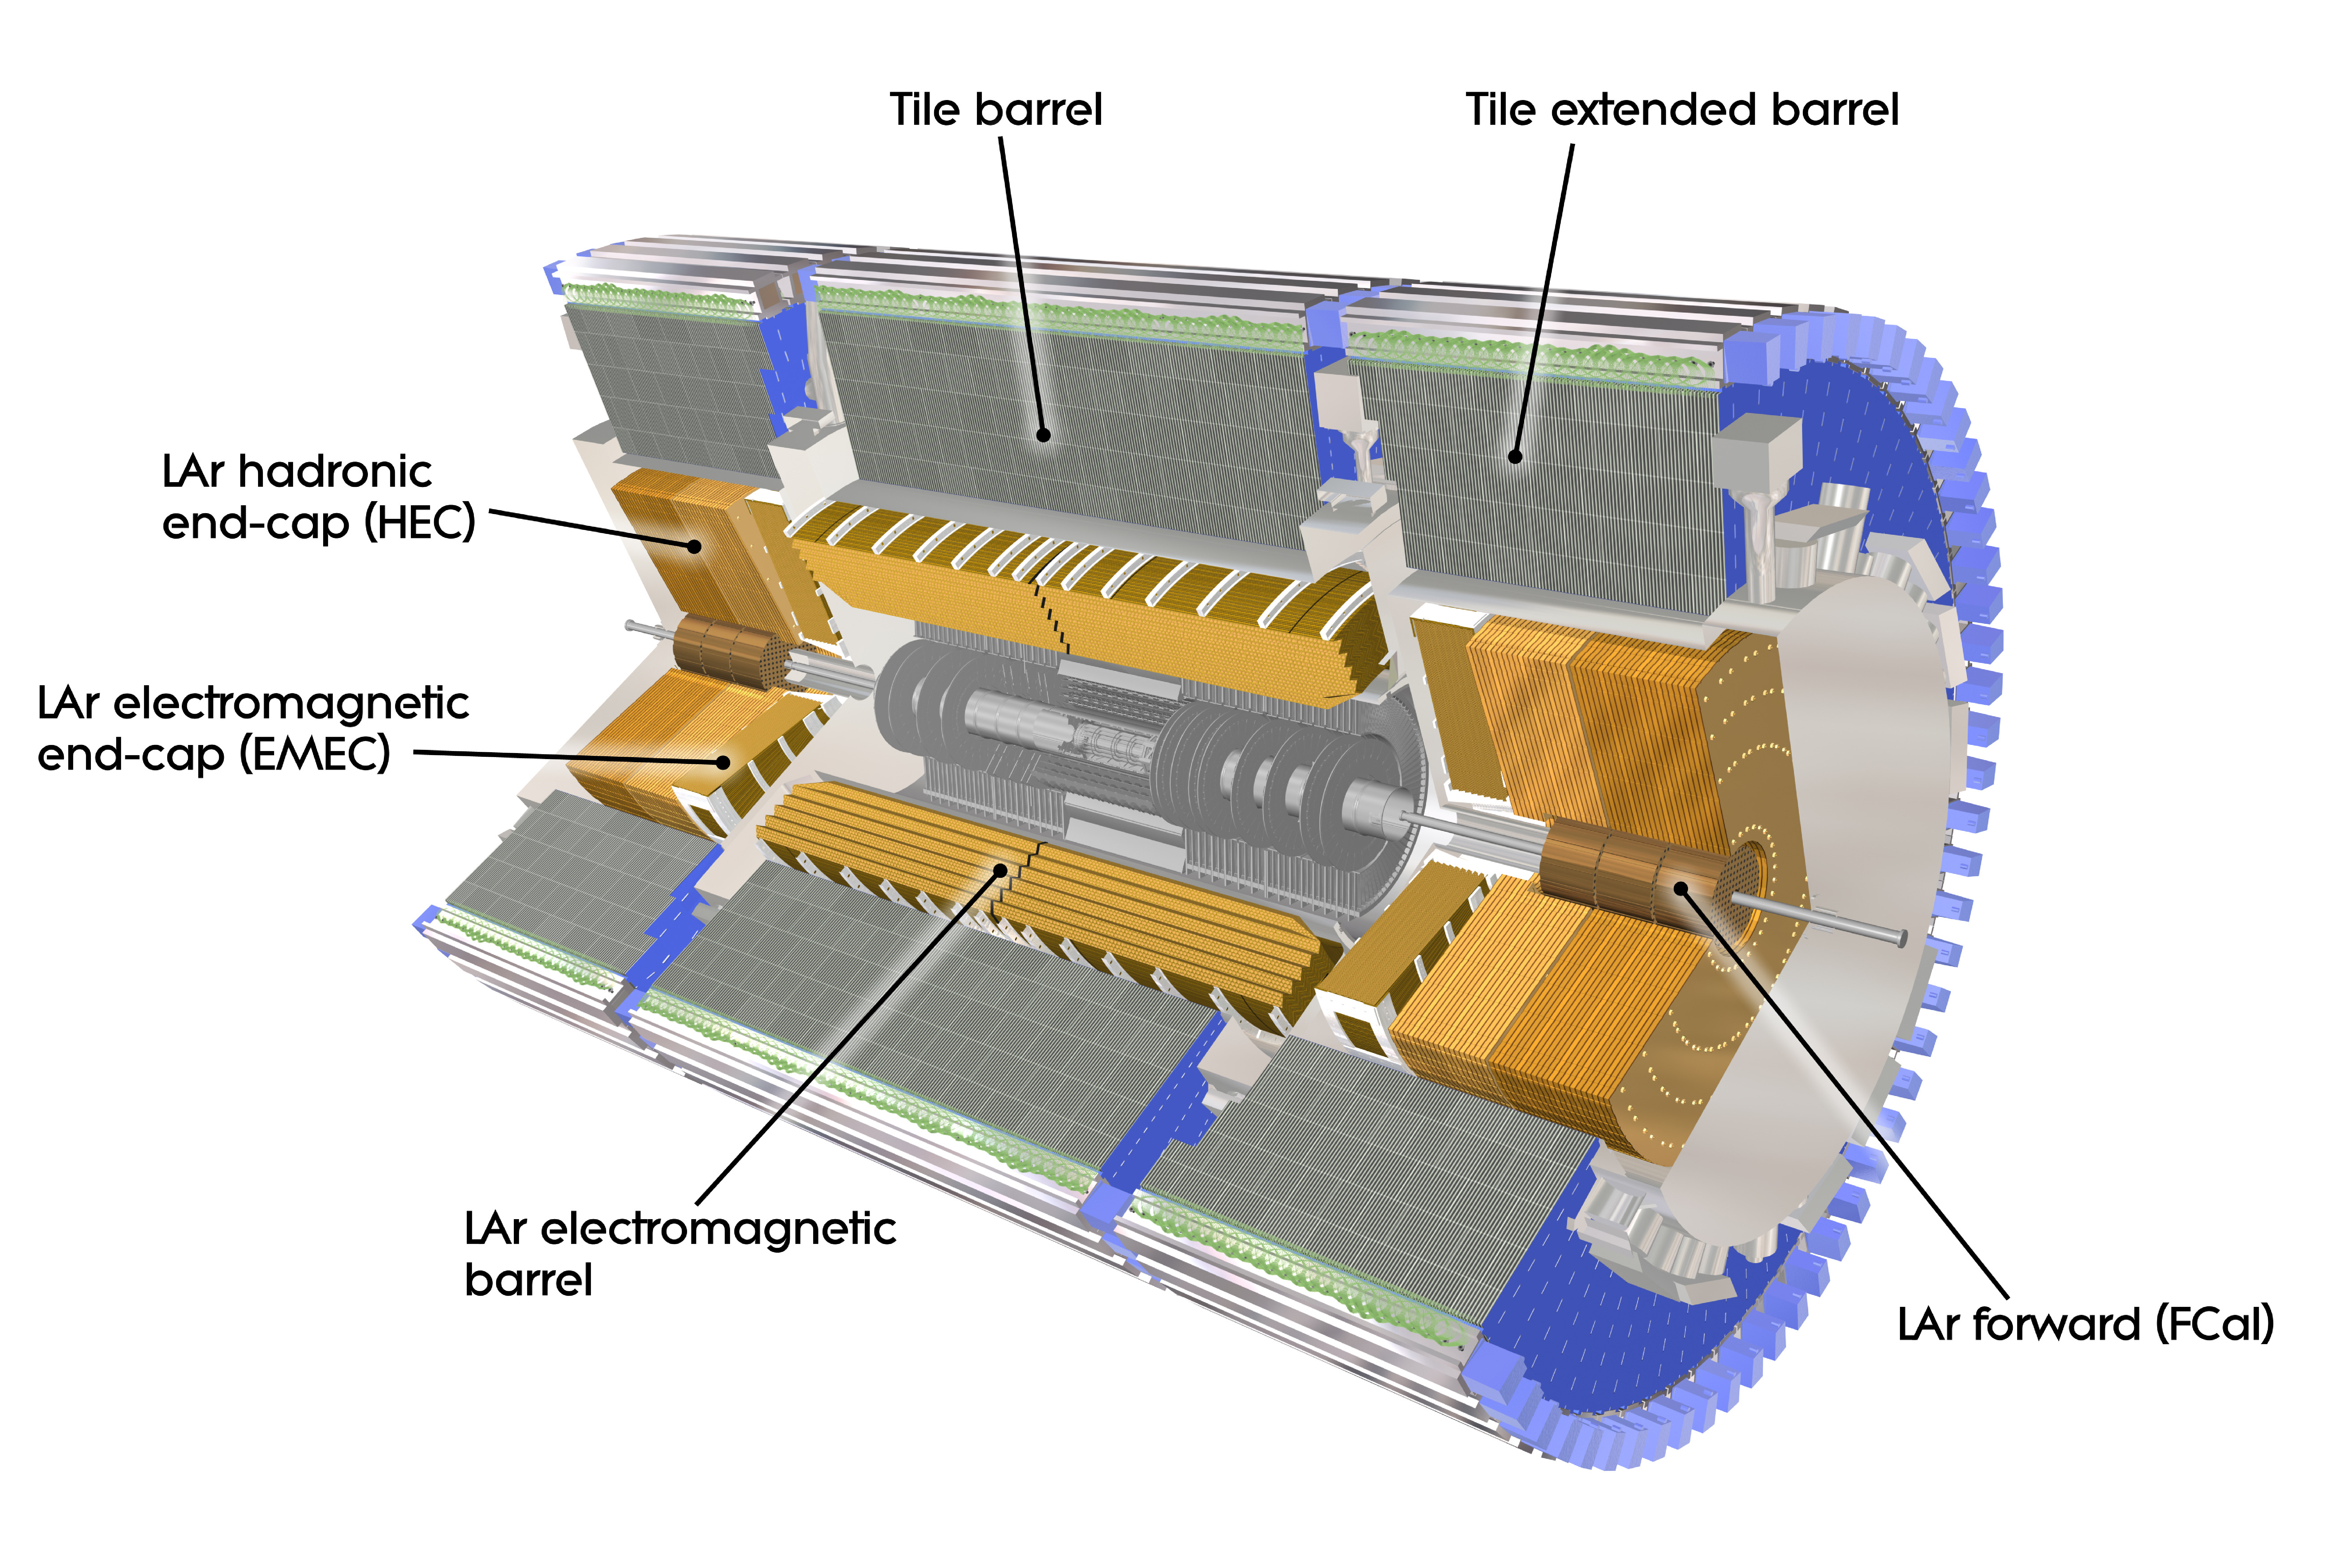
\includegraphics[width=\textwidth]{figures/calorimetros.pdf}
\caption[Os diversos subsistemas de calorimetria do ATLAS]{
Os diversos calorímetros do ATLAS. Extraído de
\cite{atlas_calorimeter_photo}.}
\label{fig:cal_atlas}
\end{figure}

O \gls{ecal} do \gls{atlas} jaz na parte mais interna do detector e cobre uma região de 
pseudorrapidez $|\gls{eta}|<3,2$. Ele pode ser dividido no
\gls{emb}, que cobre uma região pseudorrapidez de $|\gls{eta}|<1,475$, 
e por suas \glspl{emec}, cobrindo por sua vez a região de $1,375<|\gls{eta}|<3,2$.

Seu \gls{hcal} cobre a mesma região de pseudorrapidez que o \gls{ecal}, envolvendo
o mesmo. O seu barril alcança até $|\gls{eta}|<1,0$, sendo adicionado uma
extensão para aumentar o alcance na região de $0,8<|\gls{eta}|<1,7$. Juntos eles
compõem o \gls{tilecal}. Finalmente, as \glspl{hec} cobrem a região de $1,5<|\gls{eta}|<3,2$. 

Um calorímetro de menor precisão, \gls{fcal}, 
é utilizado para cobrir a região mais próxima do tubo do feixe, de
$3,1<|\gls{eta}|<4,9$, compondo uma extensão ao \gls{ecal} através de sua primeira camada,  
e ao \gls{hcal} com suas segunda e terceira camadas. 

Para todas as regiões de transição entre calorímetros citadas 
há a extensão dos mesmos de modo que haja sobreposição, 
com o objetivo de evitar a queda súbita de material \cite{paper_atlas}. 

A segmentação, granularidade e número de canais (um total de $\sim190.000$) 
em cada um dos calorímetros está contida
na Tabela \ref{tab:calo}. Uma observação interessante é a queda da granularidade
conforme o aumento de \gls{eta}. Esse fato se deve a região de precisão do 
\gls{atlas} estar limitada para $|\gls{eta}| < 2,5$, consequência da capacidade do
\gls{id} de suportar radiação\fnref{fn:radiacao}. A granularidade do
\gls{hcal} é menor que a do \gls{ecal}, devido a maior largura de chuveiros
\gls{had}. Nas regiões de maior $|\gls{eta}|$, principalmente no \gls{fcal}, 
a tarefa principal do calorímetro é reconstruir jatos e medir a
\gls{Etmiss}, de modo que uma granularidade mais grosseira é aceitável.
Ainda, é possível observar um decaimento da granularidade conforme o acréscimo
das camadas de segmentação longitudinais, o que ocorre devido a expansão da
espessura lateral do chuveiro conforme a propagação do mesmo pelo calorímetro.


\subsubsection{Barril (EMB) e Tampas (EMEC) do Calorímetro Eletromagnético}
\label{par:ecal_prec}

Os \glspl{ecal} de precisão, compostos pelo \gls{emb} e \glspl{emec}, 
utilizam detectores de \gls{lar}, contendo absorvedores compostos por eletrodos 
de cobre, o seu meio ativo, enquanto o meio passivo é composto por placas de
chumbo ($\gls{X0}=0,56$~cm e $\gls{lambdaint}=17,59$~cm\footnote{Os valores de
comprimentos foram retirados de \cite{pdg_comp}.\label{fn:comp_rad_nucl}}). Eles
irão operar em uma faixa dinâmica de energia muito larga, começando em 50~MeV
e indo até os 3~TeV. Ainda, a resolução de energia desses calorímetros tem de
atender no mínimo a relação~\ref{eq:res_em}, e sua linearidade de resposta deve ser melhor 
que 0,5\% na região de energia até 300~GeV, especialmente para obter ótima 
resolução ($\sim1\%$) de massa de reconstrução dos decaimentos em elétrons e fótons 
do bóson de Higgs, os parâmetros que determinaram essas referências durante
seus projetos. 

\begin{equation}\label{eq:res_em}
\frac{\delta E}{E} \approx \frac{10\%}{\sqrt{E}} \oplus 1\%
\end{equation}

Por isso, o \gls{lar}\footnote{Para efeitos de comparação entre o meio ativo e passivo, 
os comprimentos do \gls{lar} são: $\gls{X0}=14,00$~cm e $\gls{lambdaint}=85,77$~cm.} 
foi escolhido pelo seu comportamento linear e estabilidade de resposta temporal. 
Ainda, o \gls{lar} apresenta uma resistência a radiação intrínseca, necessário
para esses calorímetros que estão na parte mais interna do detector. O sinal é gerado
através da absorção das partículas geradas pelo chuveiro que causam a ionização
do \gls{lar}. A ionização gera um par elétron-ion, e se utiliza acoplamento
capacitivo para direcionar as partículas carregadas para os eletrodos
utilizando tensões na ordem de 2~kV.

A estrutura dos calorímetros é no formato de acordeão, que permite uma cobertura
completa natural, sem fissuras (\emph{gaps}), em \gls{phi}, assim como uma extração veloz dos sinais dos eletrodos 
na parte frontal e traseira. Essa estrutura pode ser visualizada na Figura~\ref{fig:estr_acordeao}
para o barril. Já para a tampa essa estrutura é mais complexa, uma
vez que a amplitude das ondas do acordeão tem de crescer proporcionalmente ao
raio. 

%\begin{landscape}
\begin{figure}[h!t]
%\begin{sidewaysfigure}[p]
\centering
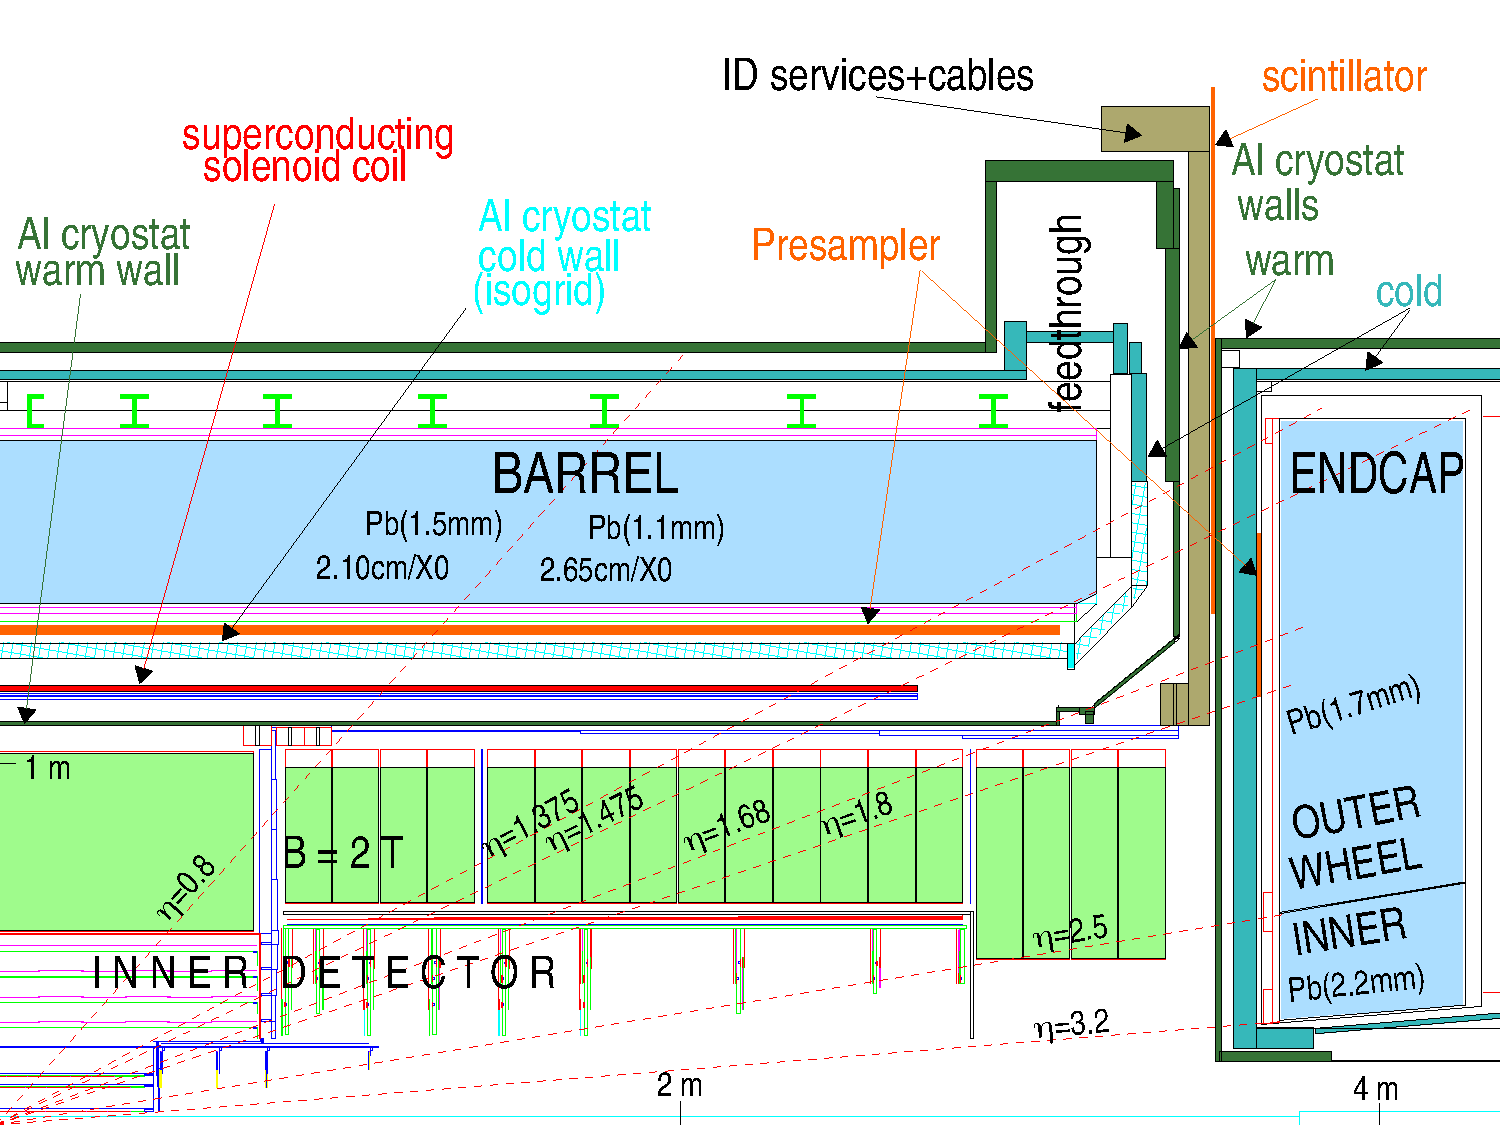
\includegraphics[width=1\textwidth]{figures/calorimetros_secao.pdf}
\caption[Seção de corte longitudinal do ECAL]
{Seção de corte longitudinal do ECAL. Extraído de
\cite{cal_tdr}}
\label{fig:secao_em_calo}
%\end{sidewaysfigure}
\end{figure}
%\end{landscape}


\begin{table}[p]\scriptsize
\centering 
\resizebox{\textwidth}{!}{
\begin{tabular}{p{5cm} c c c}
  \hline
  \hline
  \textbf{Pré-amostrador (PS)}    & \textbf{Barril}  & \textbf{Tampa} &  \\  \hline
  Cobertura   &  $|\eta|<1,52$ & $1,5<|\eta|<1,8$   \\
  Segmentação Longitudinal & 1 camada  & 1 camada  \\
  Granularidade ($\Delta \eta \times \Delta \phi$)    &  $0,025 \times 0,1$ &
$0,025 \times 0,1$  \\
  Canais de Leitura & 7808 & 1536 (ambos os lados)\\
  \hline
  \hline
  \textbf{Eletromagnético}    & \textbf{Barril}  & \textbf{Tampa (EMEC)}  \\  \hline
  Cobertura   &  $|\eta|<1,475$ & $1,375<|\eta|<3,2$   \\
  Segmentação Longitudinal & 3 camadas  & 3 camadas & $1,5   < |\gls{eta}| < 2,5$ \\
  & & 2 camadas & $1,375   < |\gls{eta}| < 1,5$ \\
  & & 2 camadas & $2,5     < |\gls{eta}| < 3,2$ \\
  Granularidade ($\Delta \eta \times \Delta \phi$)& &  \\
  Camada 1  & $0,003 \times 0,1 $  & $0.025 \times 0.1$ & $1,375 < |\gls{eta}| <
1,5$ \\ 
            &                      & $0,003 \times 0,1$ & $1,5   < |\gls{eta}| <
1,8$ \\
            &                      & $0,004 \times 0,1$ & $1,8   < |\gls{eta}| <
2,0$ \\
            &                      & $0,006 \times 0,1$ & $2,0   < |\gls{eta}| <
2,5$ \\
            &                      & $0,1   \times 0,1$ & $2,5   < |\gls{eta}| <
3,2$ \\

  Camada 2  & $0,025 \times 0,025$ & $0,025 \times 0,025$   & $1,375 <
|\gls{eta}| < 2,5$ \\
            &                      & $0,1 \times 0,1$      & $2,5   <
|\gls{eta}| < 3,2$ \\
  Camada 3  & $0,050 \times 0,025$ & $0,050 \times 0,025$  & $1,5   <
|\gls{eta}| < 2,5$ \\
  Canais de Leitura & 101760 & 62208 (ambos os lados)\\
   \hline
   \hline
  \textbf{Had. Telhas Cintilantes (\emph{TileCal})}    & \textbf{Barril}  & \textbf{Barril
estendido}     \\  \hline
  Cobertura   &  $|\eta|<1,0$ & $0,8<|\eta|<1,7$   \\
  Segmentação Longitudinal & 3 camadas  & 3 camadas  \\
  Granularidade ($\Delta \eta \times \Delta \phi$)& &  \\
  Camadas 1, e 2    &  $0,1 \times 0,1$ & $0,1 \times 0,1$   \\
  Camada 3   &  $0,2 \times 0,1$ & $0,2 \times 0,1$   \\
  Canais de Leitura & 5760 & 4092 (ambos os lados)\\
  \hline
  \hline
  \textbf{Had. Argônio Líquido (HEC)}    &  &  \textbf{Tampa}     \\  \hline
  Cobertura   &   & $1,5<|\eta|<3,2$  \\
  Segmentação Longitudinal &   & 4 camadas  \\
  Granularidade ($\Delta \eta \times \Delta \phi$)& & $0,1 \times 0,1 $ & $1,5 <
|\gls{eta}| < 2,5$ \\
  & & $0,2 \times 0,2 $ & $ 2,5 < |\gls{eta}| < 3,2$ \\
  Canais de Leitura & & 5632 (ambos os lados)\\
  \hline
  \hline
  \textbf{Calorímetro Dianteiro (FCal)}    &  &   \textbf{Dianteiro}    \\  \hline
  Cobertura   &  & $ 3,1 < |\gls{eta}| < 4,9 $ \\
  Segmentação Longitudinal &   & 3 camadas  \\
  Granularidade ($\Delta \eta \times \Delta \phi$)& & $\sim0,2 \times 0,2$  \\
  Canais de Leitura & & 1762 (ambos os lados)\\
  \hline
  \hline
\end{tabular}
}
\caption[Região de cobertura em $\eta$, granularidade e
número de canais de leitura das camadas dos calorímetros]
{Região de cobertura em $\eta$, granularidade e
número de canais de leitura das camadas dos calorímetros. Adaptado de
\cite{tese_eduardo}}
\vspace{.3cm}
\label{tab:calo}
\end{table}



Um corte longitudinal do \gls{ecal} está disposto na
Figura~\ref{fig:secao_em_calo}. Devido a complexidade da geometria do
calorímetro, existem três regiões de fissuras, também simétricas em \gls{phi}, 
nas quais a resposta do detector é degradada em comparação com o resto 
da cobertura. São elas:

\begin{itemize}
\item $\gls{eta}=0$ : entre a junção das duas metades do barril, existe uma 
pequena fissura totalizando 6~mm de \gls{lar} inativo;
\item $|\gls{eta}|\sim1,45$ : a região de transição entre o barril e a tampa é
utilizada como trajeto para os cabos e serviços do \gls{id}. Essa região é a
maior fissura do detector, começando a degradar lentamente a resposta do detector em
$|\gls{eta}|>1,35$, e indo até cerca de $|\gls{eta}|<1,68$;
\item $|\gls{eta}|=2,5$ : na região de transição entre a tampa mais externa e
interna do detector uma pequena fissura de 3~mm. Uma degradação adicional é
causada por um material morto colocado na frente deste local como um anel de
suporte.
\end{itemize}

A estrutura de acordeão
tem como vantagem a flexibilidade de segmentação longitudinal e transversa,
permitindo a implementação de camadas com diferentes granularidades. São
utilizadas três camadas, que podem ser observadas na
Figura~\ref{fig:cal_lar_camadas}, com as seguintes propriedades:

\begin{figure}[h!t]
\centering
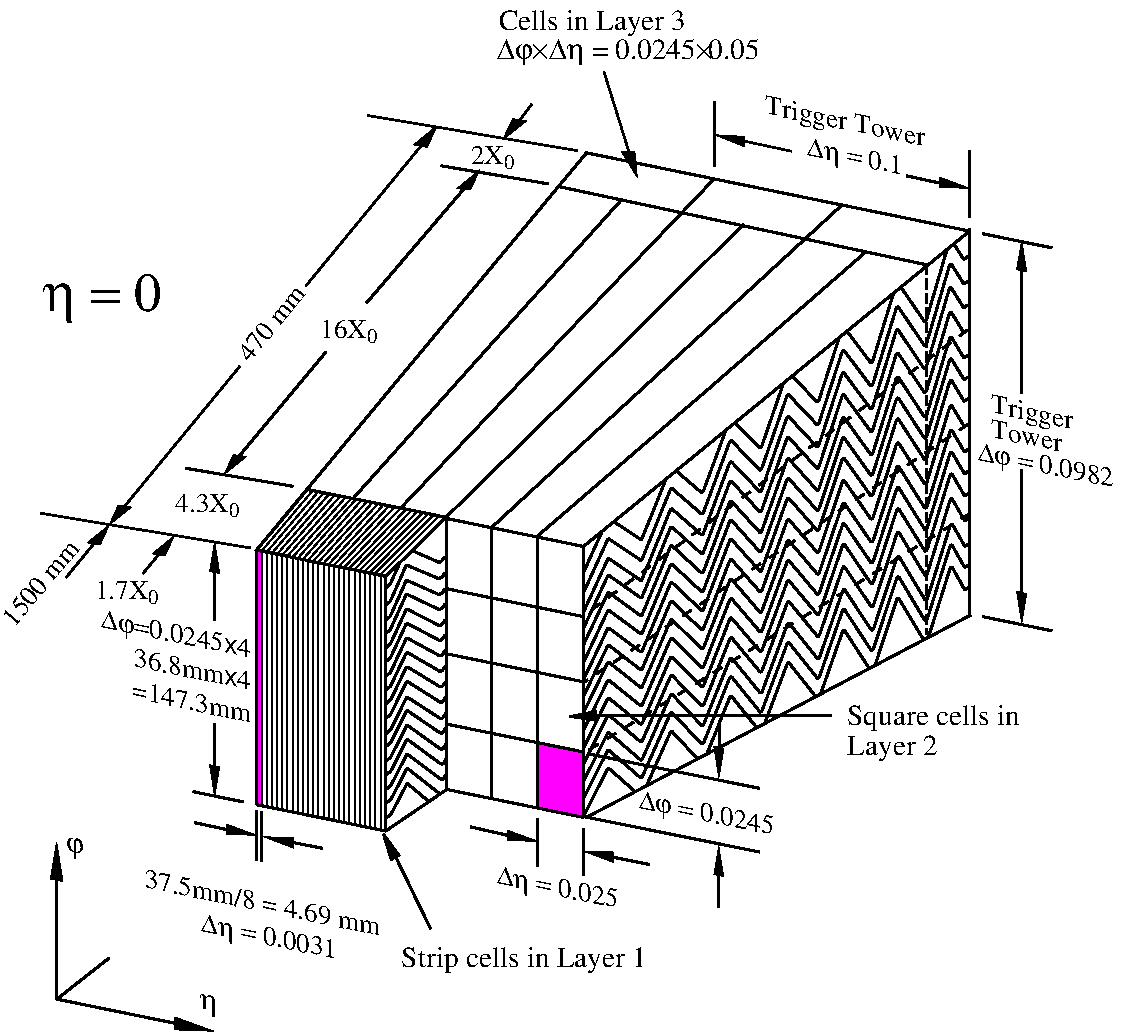
\includegraphics[width=.6\textwidth]{figures/cal_lar_camadas.pdf}
\caption[Esboço da estrutura do acordeão e a granularidade de suas camadas para
o EMB]{Esboço da estrutura de acordeão e a granularidade de suas camadas para
$|\eta|=0$ do EMB. A quantidade de $X_0$ típicos para cada uma das camadas também é
mostrada. Extraído de \cite{cal_tdr}.}
\label{fig:cal_lar_camadas}
\end{figure}

\begin{itemize}
\item \textbf{\gls{e1}}: a primeira camada é composta por tiras
finas com grande granularidade em \gls{eta}, tendo como objetivo fazer uma
boa leitura dessa posição. Isso é especialmente importante no caso de fótons,
que não são medidos pelo detector de traços, e ao mesmo tempo para casar os
traços das partículas com seus respectivos chuveiros. Conforme o \gls{eta} aumenta,
há um decréscimo da granularidade devido ao fato das tiras não poderem ser feitas com menos de 5~mm.
A escolha de tiras mais grosseiras em \gls{phi} quando comparadas com a segunda e 
terceira camadas é consequência do campo magnético do \gls{cs} espalhar os
chuveiros em \gls{phi} que possam ocorrer antes do calorímetro.


\item \textbf{\gls{e2}}: a segunda camada é responsável pela
absorção da maior quantidade de energia. Ela é segmentada transversalmente em
torres quadradas de $(\Delta\eta\times\Delta\phi)\approx(0,025\times0,025)$, que
permitem um compromisso ótimo entre a contenção do perfil lateral do chuveiro
com a contribuição do ruído por Empilhamento e eletrônico para a medição de
energia.

\item \textbf{\gls{e3}}: a terceira camada tem a mesma
granularidade que a central em \gls{phi}, mas sua granularidade é duas vezes mais grosseira
em \gls{eta}. Ela é utilizada para separar chuveiros de altas energias, e
contribui para a separação de $\gamma/$jato e elétron/jato. No caso da tampa
para $|\gls{eta}|>2,5$ são utilizadas apenas duas camadas com granularidade mais
grosseira, uma vez que se está fora da região de precisão.
\end{itemize}

Para fazer a medição com precisão da energia é necessário o mínimo de material 
antes de sua medição, de modo que essa não seja prejudicada pela geração de
chuveiros antes dos calorímetros, o que causaria a perda de energia das
partículas e deteriorando, simultaneamente, a precisão da posição de impacto 
da partícula com o mesmo. Por mais que todo o material colocado antes do
calorímetro tenha sido otimizado para minimizar esse efeito, ainda assim é
possível que isso ocorra, de modo que um instrumento Pré-amostrador foi colocado 
para estimar a perda de energia no material existente antes do calorímetro, 
estando descrito no Subtópico~\ref{par:cal_ps}.



\begin{figure}[ht!]

    \begin{center}
    
        \subfigure[Valores de $X_0$ em função de $\eta$ para as diferentes camadas do ECAL e outros materiais dispostos antes do mesmo.]
         {
            \label{fig:cal_em_x0}
            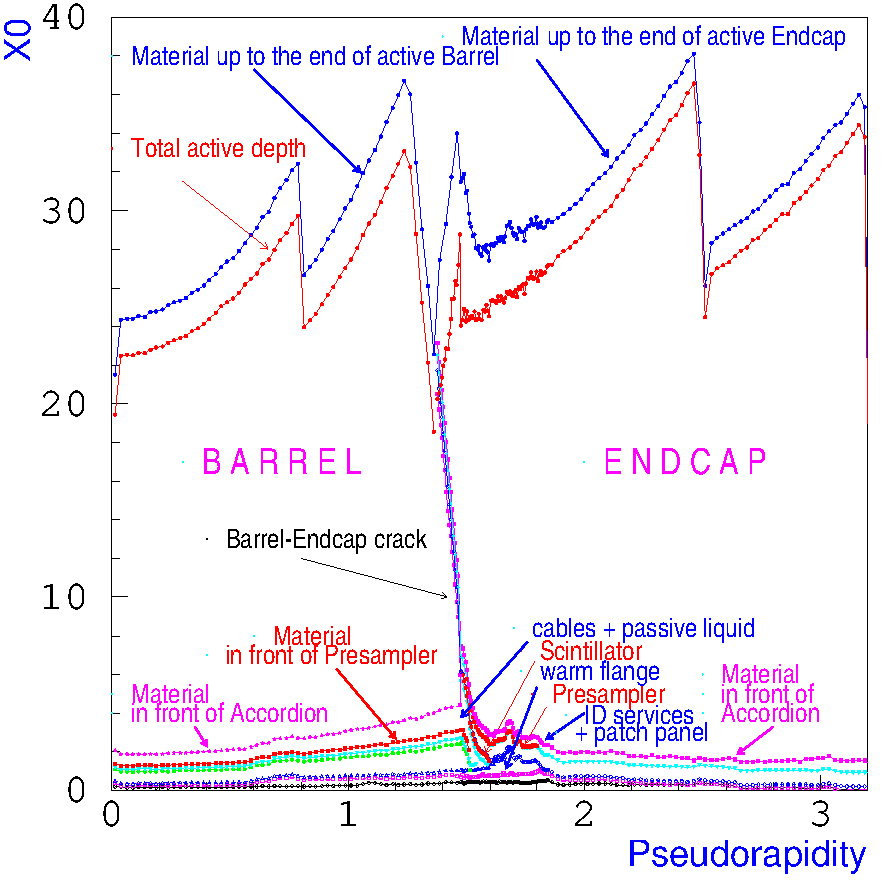
\includegraphics[width=0.46\textwidth]{figures/cal_em_x0.pdf}
        }\hspace{0.02\textwidth}
        \subfigure[Valores de $\lambda_{int}$ em função de $\eta$ para as diferentes camadas e subsistemas do calorímetro]
        {
            \label{fig:cal_had_lambda}
            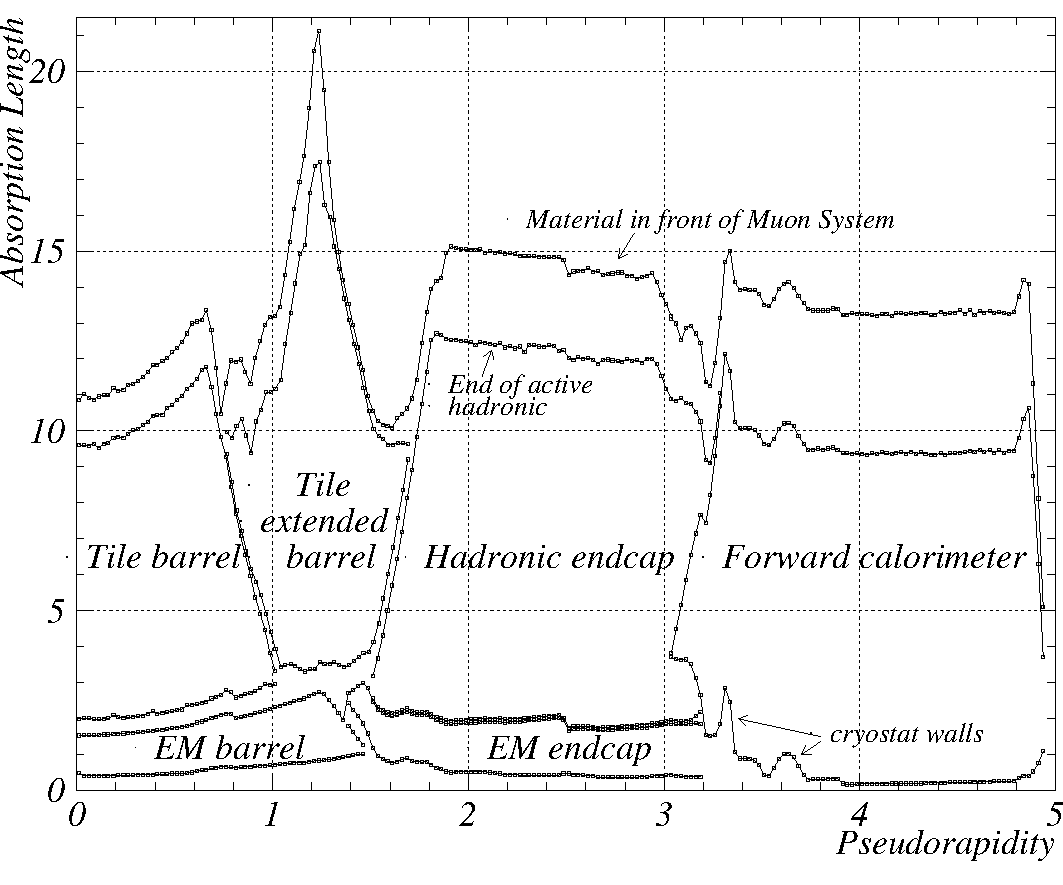
\includegraphics[width=0.46\textwidth]{figures/cal_had_lambda.pdf}
        }\\ 

    \end{center}
    
    \caption[Valores de $X_0$ e $\lambda_{int}$ em função de $\eta$ para as diferentes camadas e subsistemas.]
    {Valores de $X_0$ e $\lambda_{int}$ em função de $\eta$ para as diferentes
camadas e subsistemas. Extraído de \cite{cal_tdr}.}

\end{figure}


O \gls{ecal} tem de ser capaz de absorver completamente a energia
das partículas que devem variar de 50~MeV até 3~TeV. 
Para absorver as partículas com maiores energias, o \gls{ecal} conta com valores
maiores a 24~\gls{X0} no barril, e maiores a 26~\gls{X0} na tampa. Os valores de \gls{X0} em 
função de \gls{eta} estão dispostos na Figura~\ref{fig:cal_em_x0}, onde também é possível
visualizar os valores desse parâmetro para os materiais localizados antes do
calorímetro.

\subsubsection{Calorímetro Hadrônico de Telhas (\emph{TileCal})}
\label{par:cal_tilecal}

No barril do \gls{hcal}, chamado de \gls{tilecal}, o meio de amostragem consiste de telhas de
cintiladores de plástico e seu material passivo é o aço (o \gls{lambdaint} é
aproximadamente igual ao do chumbo, cerca de $16,8$~cm\fnref{fn:comp_rad_nucl}), Figura~\ref{fig:estr_tilecal}. 
Ao invés do efeito capacitivo utilizado no \gls{lar}, os cintiladores de
plástico são excitados pelas partículas carregadas do chuveiro, de modo que são
emitidos fótons capturados por fibras óticas, que os direcionam aos
\glspl{pmt}. Os \glspl{pmt} geram um sinal proporcional a energia da partícula
que iniciou o chuveiro.
Essa técnica de amostragem é utilizada pois nesta região mais externa e central do detector 
há pouca incidência de radiação\footnote{Uma relação entre a incidência de
radiação e pseudorrapidez foi feita em Seção~\ref{ssec:det_int}.\label{fn:radiacao}}, 
sendo possível utilizar um método com menor custo financeiro.

O \gls{tilecal} é segmentado longitudinalmente para garantir melhor identificação
das partículas, e pela possibilidade de conseguir uma melhor resolução de
energia através da calibração realizada pela ponderação do depósito em cada um
das camadas. São utilizadas três camadas para esse propósito: \gls{h0}, \gls{h1} 
e \gls{h2}.

A resolução de energia do calorímetro necessária para fazer a medição dos
diversos jatos e hádrons gerados nas colisões e dos jatos duplos provenientes 
dos decaimentos do bóson W tem de atender \ref{eq:res_tile1}. 
A linearidade de resposta do calorímetro mínima é de 2\% em uma escala de até 4
GeV.

\begin{equation}\label{eq:res_tile1}
\frac{\delta E}{E} \approx \frac{50\%}{\sqrt{E}} \oplus 3\% \;\ \text{para} \;\
|\gls{eta}|<3
\end{equation}

É necessário que o \gls{hcal} tenha no mínimo a espessura de 10 \gls{lambdaint}
para a contenção completa dos chuveiros, tanto para garantir resolução de
energia, quanto reduzir o ruído causado no Espectrômetro de Múons. Os valores de
\gls{lambdaint} para os diversos \gls{hcal} estão dispostos na
Figura~\ref{fig:cal_had_lambda}.


\subsubsection{Tampas do Calorímetro Hadrônico (HEC)}
\label{par:cal_hec}

Para a \gls{hec} também se utiliza o \gls{lar} como meio ativo devido a
incidência de radiação, mas ao invés de chumbo, seu material passivo é o cobre
($\gls{X0} = 1,43$~cm e $\gls{lambdaint}=9,39$~cm\fnref{fn:comp_rad_nucl}). 
Sua estrutura foi projetada como uma chapa plana 
demonstrada na Figura~\ref{fig:estr_hec}. São utilizadas duas tampas para cada
\gls{hec} contendo cada uma 32 módulos idênticos. Cada módulo consiste de 24
chapas de cobre para a primeira tampa, e 16 chapas para a segunda. Em ambos os
casos as chapas de cobre estão separadas por uma fissura de 8,5~mm contendo
\gls{lar} e três eletrodos. Essa estrutura foi escolhida principalmente por ter
uma maior resistência a radiação e eficácia de custo, ainda fornecendo a
cobertura espacial necessária.

Os requisitos de linearidade e de resolução de energia devem atender aqueles
especificados para o \gls{tilecal}. Ainda, um tempo de pico de sinal
de $\sim40$ ns deve ser atendido pelo \gls{lar}. O número de \gls{lambdaint} da
\gls{hec} em função de $\gls{eta}$ estão na Figura~\ref{fig:cal_had_lambda}.

Diferente do barril, a tampa do \gls{hec}
possui 4 camadas, mas normalmente as duas camadas centrais são agrupadas em uma
única camada, de forma a manter a uniformidade de segmentação longitudinal do
\gls{hcal}.

\subsubsection{Calorímetro Dianteiro (FCal)}
\label{par:cal_fcal}

Já o \gls{fcal} apresenta uma estrutura diferenciada
para aguentar os elevados índices de radiação próximos ao tubo do feixe. Em sua primeira camada, 
é utilizada uma matriz de metal absorvedora de cobre contendo buracos igualmente
distribuídos. Nesses buracos são colocados uma estrutura de hastes coaxiais e tubos, 
ambos novamente de cobre, separados por um preciso pedaço de fibra de plástico resistente
a radiação. A matriz e o tubo compõem o material passivo,
enquanto o espaço remanescente entre o tubo e a haste é preenchido por \gls{lar},
o meio de amostragem. O tubo está aterrado, enquanto as hastes estão em alta tensão, 
criando o efeito capacitivo.
Essa estrutura fica mais facilmente compreendida na Figura~\ref{fig:estr_fcal}. 
O material das hastes e da matriz são substituídos de cobre para tungstênio
($\gls{X0} = 0,350$~cm e $\gls{lambdaint} = 5,72$~cm\fnref{fn:comp_rad_nucl}) com 
o objetivo de elevar a capacidade de absorção de partículas \gls{had} nas segunda 
e terceira camadas. O acumulo de íons de \gls{lar} nas fissuras limita a
luminosidade máxima proporcionalmente a $1/g^2$, de forma que o comprimento das
fissuras (g) devem ser os menores possíveis. 
As dimensões das mesmas são de 250-375~$\mu$m para a seção \gls{em} 
e 500~$\mu$m para a seção \gls{had}.


A tarefa principal desse detector é a reconstrução de jatos e fornecer
hermeticidade para a medição de \gls{ptmiss}. Por isso, a resolução de energia para 
o \gls{hcal} na região dianteira pode ser menor, de
acordo com a Equação~\ref{eq:res_tile2}. Nessa região, também, é necessária a identificação de
jatos dianteiros uma vez que a região de admissão para seus decaimentos do
bóson de Higgs é de $2<|\gls{eta}|<5$. Observe novamente a
Figura~\ref{fig:cal_had_lambda} para os comprimentos do \gls{fcal}.

\begin{equation}\label{eq:res_tile2}
\frac{\delta E}{E} \approx \frac{100\%}{\sqrt{E}} \oplus 10\% \;\ \text{para} \;\
3<|\gls{eta}|<5
\end{equation}



\begin{figure}[ht!]
    \label{fig:estruturas_cal}
    \begin{center}

        \subfigure[Acordeão para o barril do ECAL. Extraído de \cite{cal_tdr}.]{
            \label{fig:estr_acordeao}
            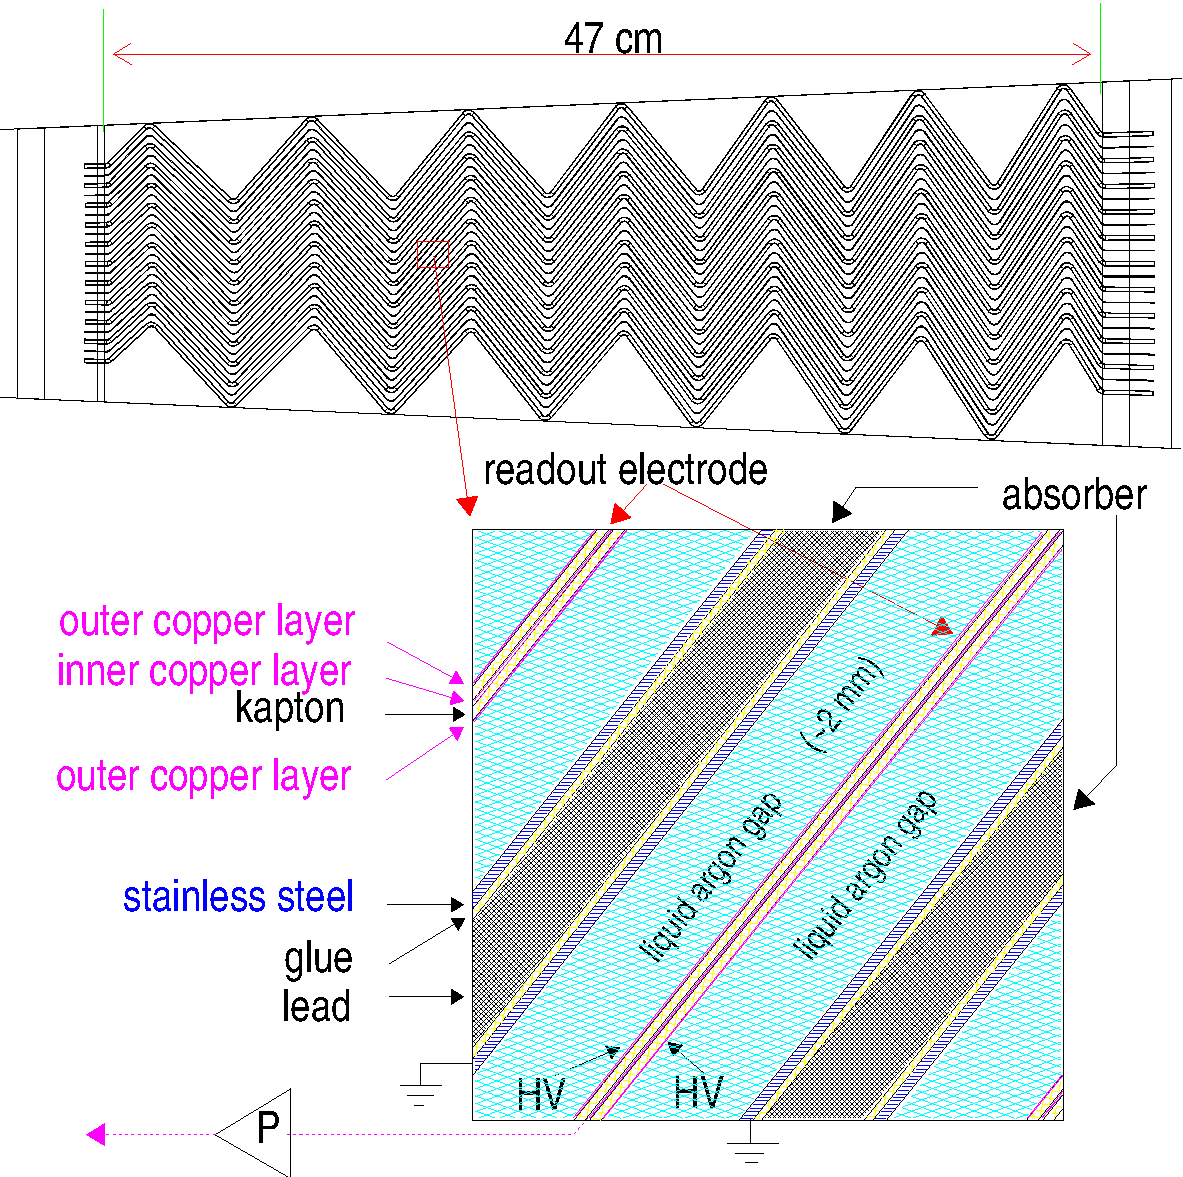
\includegraphics[width=.46\textwidth]{figures/estrutura_acordeao_barril.pdf}
        } \hspace{0.01\textwidth}
        \subfigure[Telhas e cintiladores do TileCal. Extraído de \cite{cal_tdr}]{
            \label{fig:estr_tilecal}
            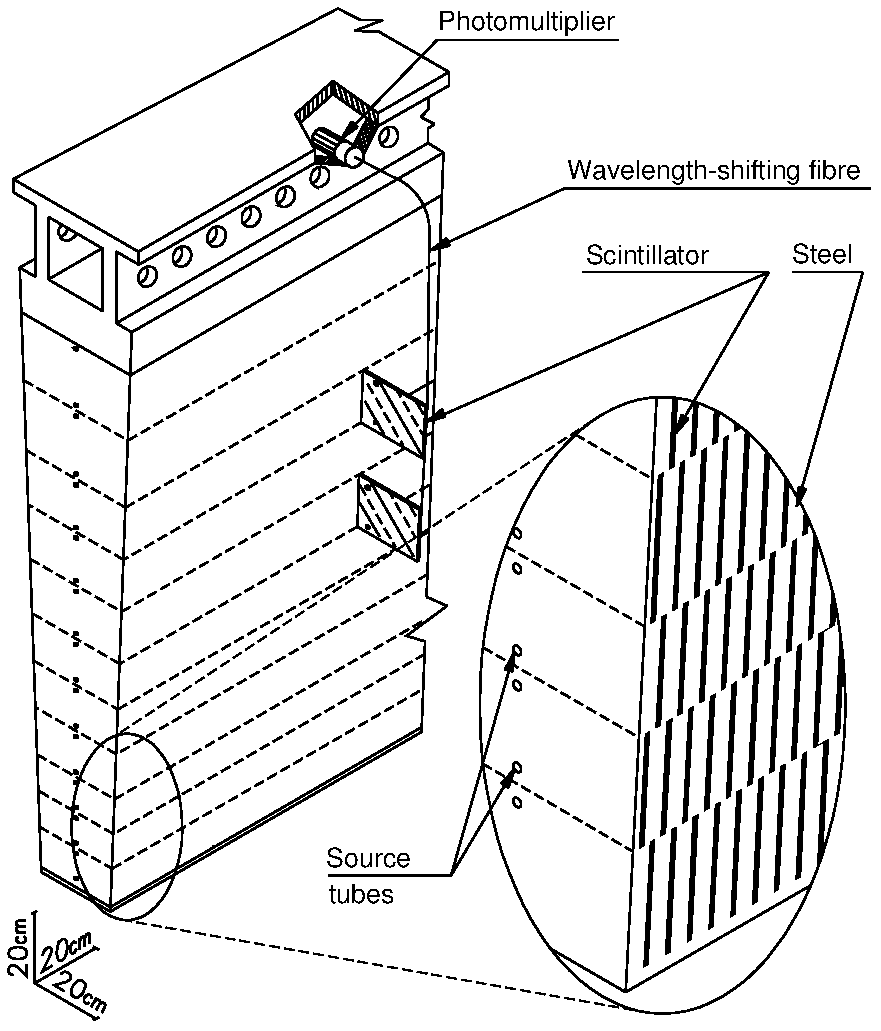
\includegraphics[width=0.46\textwidth,height=7cm]{figures/estrutura_tilecal.pdf}
        } \\
        
        \subfigure[Chapa plana do HEC. Extraído de \cite{paper_atlas}.]{
            \label{fig:estr_hec}
            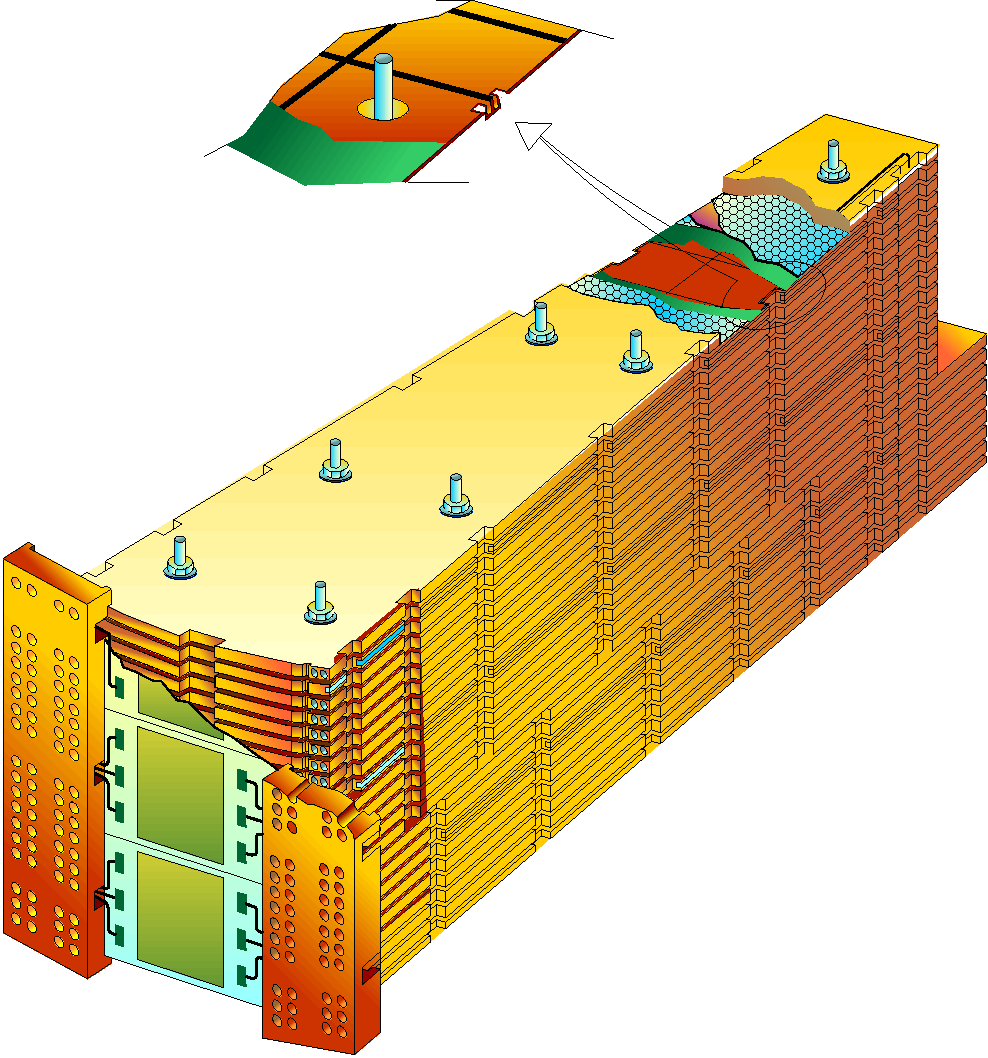
\includegraphics[width=0.46\textwidth]{figures/estrutura_hec.pdf}
        }\hspace{0.01\textwidth}
        \subfigure[Tubos e Hastes para a primeira camada do FCal. Extraído de \cite{paper_atlas}.]{
            \label{fig:estr_fcal}
            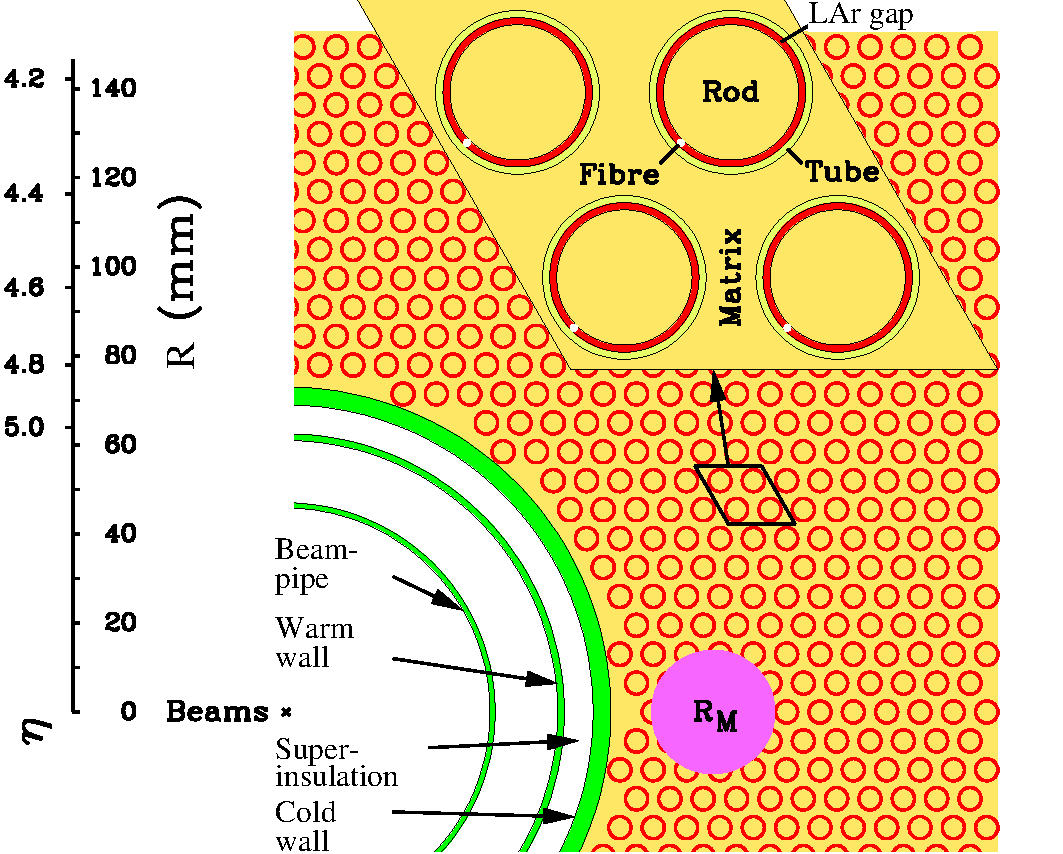
\includegraphics[width=0.46\textwidth]{figures/estrutura_fcal.pdf}
        } \\
        
    \end{center}
    \caption[As diferentes estruturas dos subsistemas de calorimetria do ATLAS]{As diferentes estruturas dos subsistemas de calorimetria do ATLAS.}
    
\end{figure}


\subsubsection{Calorímetro Pré-amostrador (PS) e Cintiladores}
\label{par:cal_ps}

O \gls{ps}, diferente dos calorímetros detalhados anteriormente, não possui meio passivo, 
constituído apenas de uma fina camada de \gls{lar} na região de
$|\gls{eta}|<1,8$. Seu barril ($|\gls{eta}|<1,52$) contém eletrodos
perpendiculares ao feixe e um comprimento de~1,1 cm, enquanto na tampa,
$1,5<|\gls{eta}|<1,8$, a configuração dos eletrodos é paralela e o comprimento
de 0,5~cm. Sua função é absorver partículas de chuveiros formados antes do
calorímetro do \gls{atlas} pela interação das partículas com o material anterior
ao calorímetro (observe os valores de \gls{X0} desses materiais na Figura~\ref{fig:cal_em_x0}), 
como no \gls{cs}, criostato e no \gls{id}. Com isso é possível realizar 
a calibração da energia perdida pelas partículas nesse material.
Além da pseudorrapidez de 1,8, o \gls{ps} não é mais 
necessário dado que o material morto (material que não contribui para a detecção
de energia da partícula) é reduzido e a energia total das partículas 
é grande para um dado \gls{pt}.

Na região de transição entre o barril e a tampa, para
$|\gls{eta}| = 1,4$, a situação é particularmente critica devido aos serviços e
cabos para o \gls{id}, e uma camada cintiladora em $1,0<|\gls{eta}|<1,6$ 
é colocada entre os dois criostatos com o objetivo de recuperar parte 
da energia perdida, principalmente por
partículas \gls{had}, mas também ajuda a reconstruir a energia de elétrons e
fótons. As disposições desses dois calorímetros, assim como do cintilador pode 
ser observada na Figura~\ref{fig:secao_em_calo}. 

\newpage
\subsection{O Espectrômetro de Múons}
\label{ssec:espectometro_muons}

Os múons como estados finais são muito importantes em diversas análises e provêm
assinaturas físicas robustas no \gls{lhc}. 
Eles penetram grandes quantidades de material enquando a maioria das outras
partículas são absorvidas, e com o objetivo de medir sua energia, o Espectrômetro
de Múons \cite{muon_tdr} é o subdetector mais externo do \gls{atlas}. Diferente dos calorímetros
que empregam um processo de medição destrutivo, o Espectrômetro de Múons,
Figura~\ref{fig:espec_muons}, mede a carga e o momento de múons através 
da reconstrução de suas trajetórias no 
campo magnético dos toroides de núcleo a ar de forma semelhante ao \gls{id}. 

\begin{figure}[h!t]
\centering
%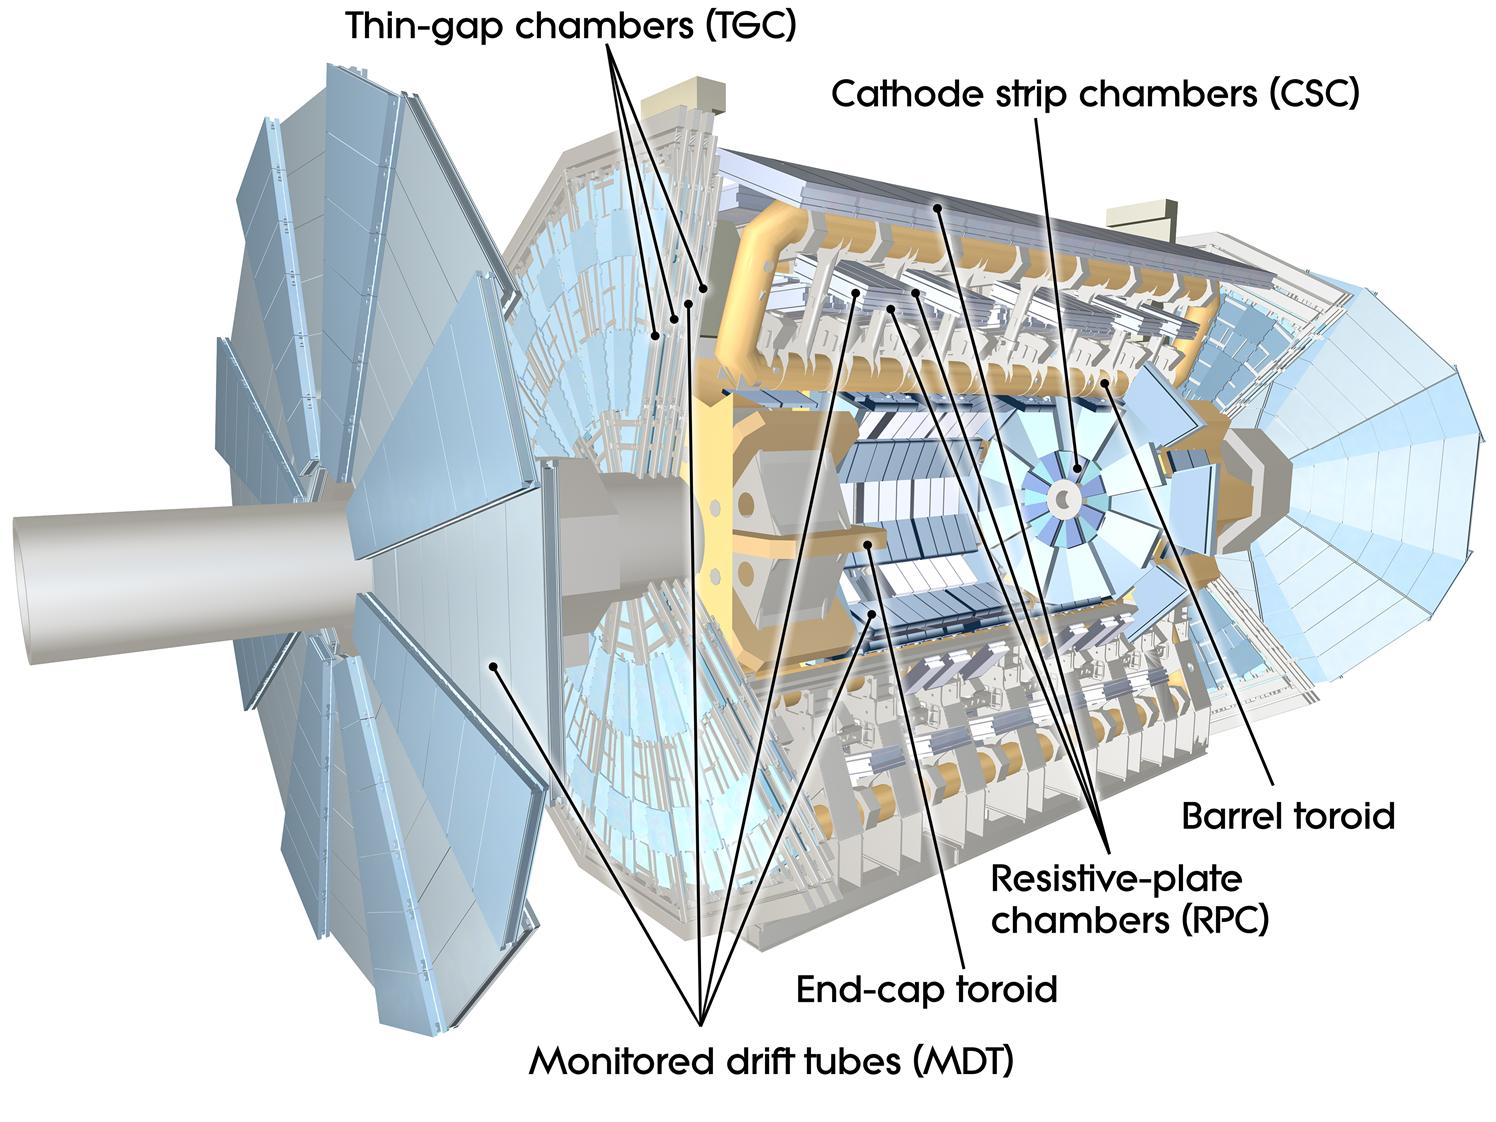
\includegraphics[width=0.8\textwidth]{imagens/espectometro_muons_lowres.jpg}
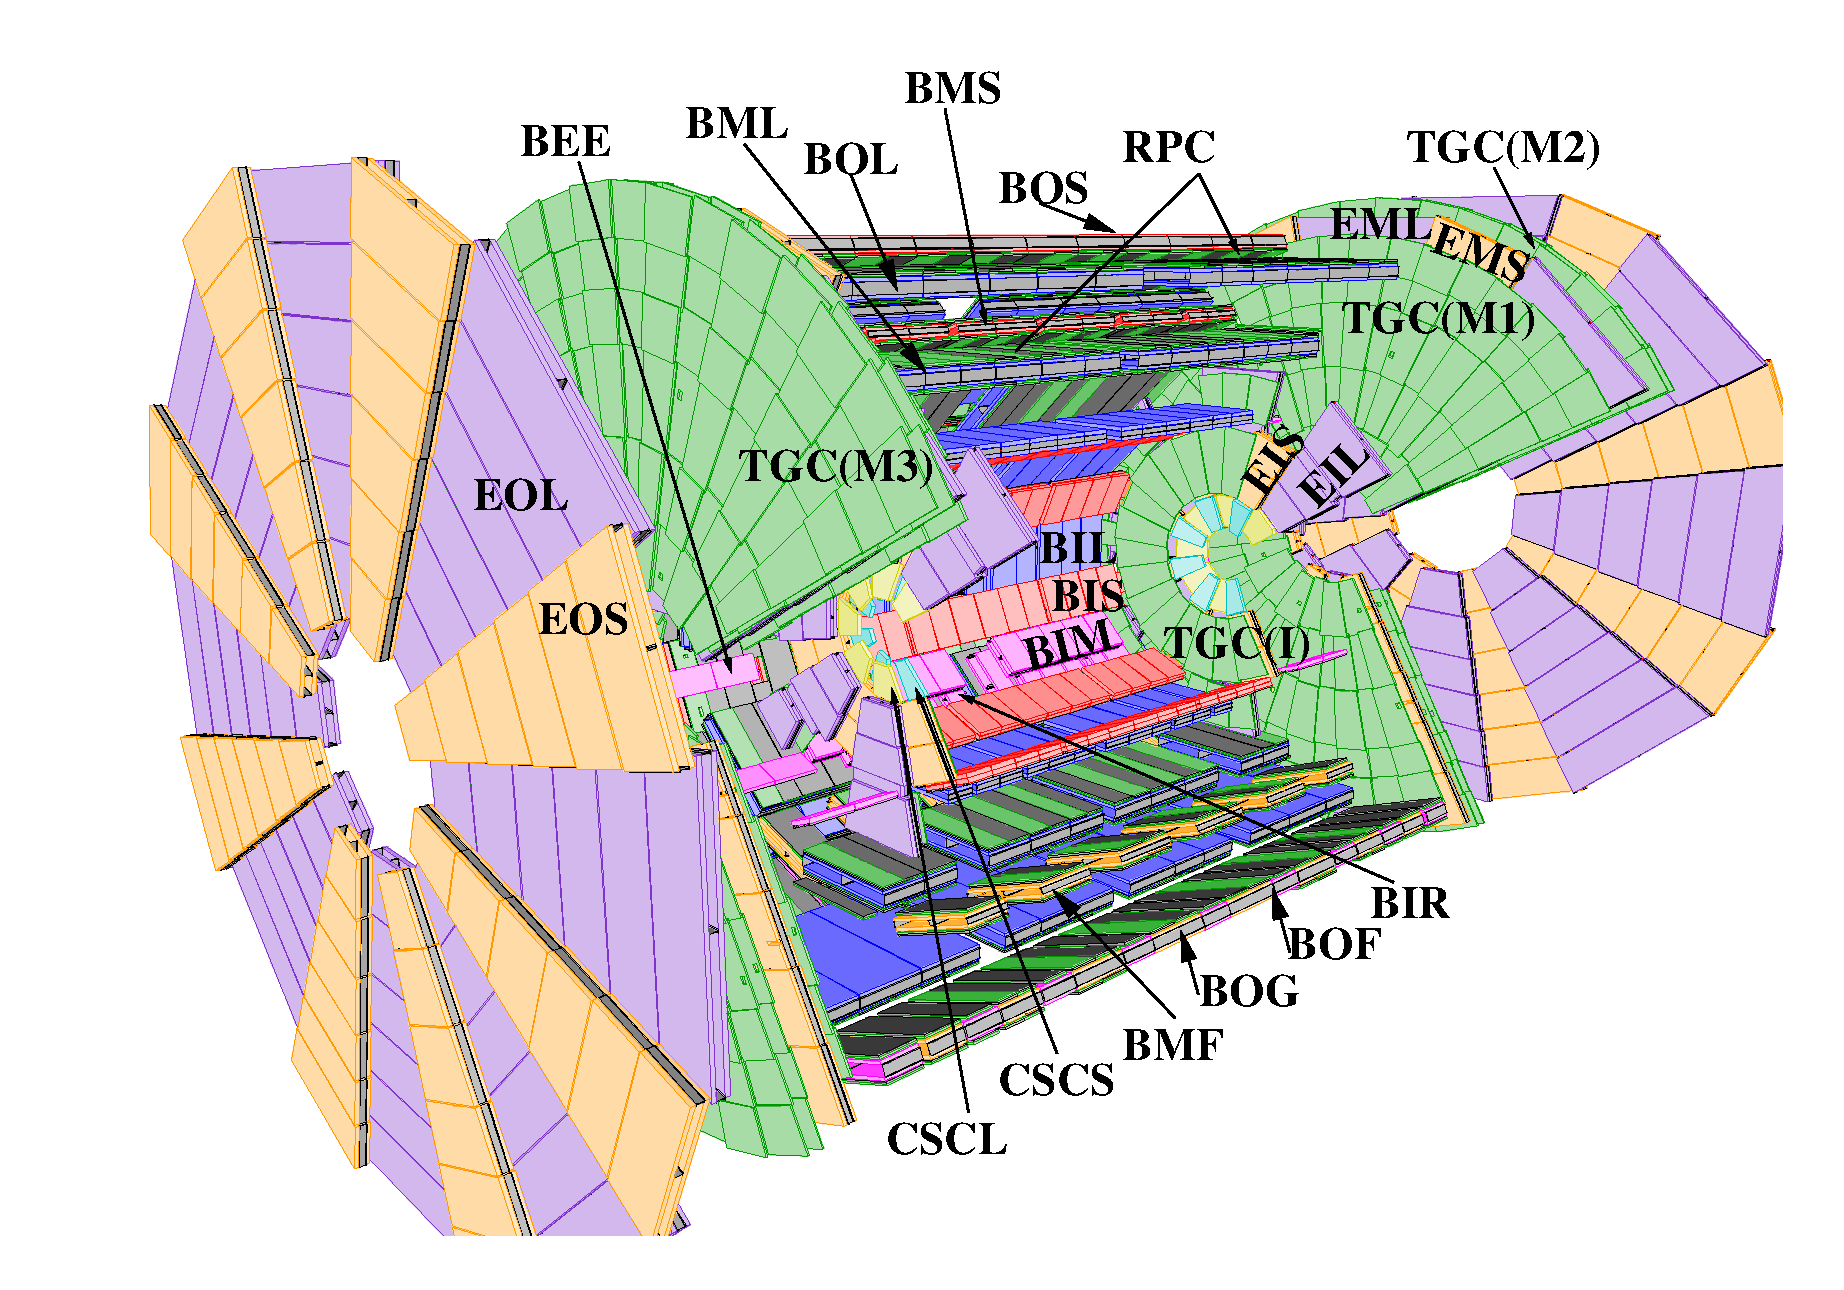
\includegraphics[width=0.7\textwidth]{figures/Muon_system_Initial.pdf}
\caption[O Espectrômetro de Múons]{
O Espectrômetro de Múons e seus subsistemas: as câmaras medidoras de
precisão: (MDTs e CSCs) e as câmaras de filtragem (RPCs e TGCs). Na tampa, a
primeira camada TGC (I) é localizada na camada mais interna; as próximas três
camadas estão na frente (M1) e atrás (M2 e M3) da segunda roda MDT. A primeira
letra (B e E) do esquema de nomenclatura do MDT faz referência às câmaras no barril
e tampa, respectivamente. A segunda e terceira letras referenciam para a camada
(interior: I, central: C, externa: O) e setor (extenso: L e pequeno: S). Extraído de
%\cite{muons_images}.}
\cite{paper_atlas}.}
\label{fig:espec_muons}
\end{figure}

As câmaras no barril formam três cilindros
concêntricos com o eixo dos feixes e cobrem um alcance em $|\gls{eta}| < 1$,
estando localizadas a uma distância radial de $\sim$5, 7,5, e 10~m. São
utilizados quatro discos para as câmaras da tampa que cobrem um o alcance de 
$1 < |\gls{eta}| < 2,7$ em distâncias de $\sim$7, 10, 14 e 21-23~m do ponto de
interação, todos concêntricos ao tubo do feixe. Deseja-se medir múons
na região de poucos GeV com uma resolução de $\sim1\%$, enquanto para múons na
faixa de 1 TeV a precisão pode ser um pouco menor ($ < 10\%$). O poder de
curvatura $Bl^2$ fornecido pelos toroides e tamanho do detector é de cerca de 36~$\text{Tm}^2$, 
comparado com os 2~$\text{Tm}^2$ no \gls{id}. Para fornecer a
resolução de momento desejada a \gls{respos} deve ser de no mínimo
50~$\mu$m em z e 0,5~mrad em R$\phi$ \cite{ATLAS_TDR}.

Existem diversos tipos de câmaras de traços de múons: As \gls{mdt} e \gls{csc}
são as câmaras de precisão, já as \gls{rpc} e \gls{tgc} são câmaras
rápidas para o \glslink{l1}{Primeiro Nível de filtragem (L1)}. O princípio de leitura é o mesmo para os quatro
tipos, onde os múons que passam por uma fenda de gás entre um anodo e catodo (por
exemplo, um cabo dentro de um tubo ou duas chapas paralelas) causam uma descarga
local no gás sendo assim possível ler o sinal. No total existem 5376 câmaras
com 1,0757~M canais de leitura \cite{tese_jatos}.

Os \glspl{mdt} fornecem medições de precisão (acurácia mecânica de 30~$\mu$m) 
dos pontos do traço com 80~$\mu$m de \gls{respos}
para cada cabo em uma larga região de \gls{eta}. Em grandes \gls{eta} e próximo
do ponto de interação são utilizados os \glspl{csc}, que têm uma maior
granularidade e suportam a sua alta demanda causada pelas condições de ruído
físico.
 
As câmaras de filtragem têm uma resolução de tempo menor que o espaçamento
mínimo entre pacotes de 25~ns para fazer possível sua identificação. Os
requisitos de tempo e espaço são atendidos de acordo com a seguinte
especificação: os \glspl{rpc} têm boa resolução de tempo (1,5~ns), por outro
lado os \glspl{tgc} tem melhor resolução espacial 
(o afastamento entre os cabos anodos é de 1,8~mm).

Graças a grande dimensão do Espectrômetro de Múon não é possível de firmar as
dimensões e posições das câmaras no nível requerido de 30~$\mu$m. Portanto, as
deformações e posições da câmara são constantemente monitoradas por meio de
sistemas ópticos de alinhamento, de forma que deslocamentos dentre $\sim$30~$\mu$m e $\sim$1~cm 
podem ser corrigidos em análise pelos algoritmos do
\glsdesc{sr} \cite{muon_tdr}.














\chapter{Sistema de Filtragem de Eventos do ATLAS}
\label{cap:trigger}
\glsresetall


A maioria das reações de interresse ocorrem com frequência bastante reduzida, uma vez que esses
eventos são bastante raros. Por outro lado, jatos hadrônicos possuem uma frequência da ordem de centenas de $k$Hz, sendo necessários
descartá-los da cadeia de processamento. Além da taxa de colisões, a granularidade dos detectores 
envolvidos na aquisição dos eventos colabora, de forma crucial, com o volume de informação gerado.

À cada colisão, aproximadamente 1,5 MBytes de informação serão 
produzidos.  Ao multiplicar-se este valor pela taxa de colisões, obtém-se um volume de informação da ordem de 60 TBytes por segundo. 
Adicionalmente, canais físicos de interesse ocorrem com um período que varia de algumas horas a até dias de operação. 
Consequentemente, um sistema de filtragem online torna-se indispensável para o experimento. O sistema de filtragem deverá identificar os 
padrões de decaimento do \textit{Higgs}, e demais eventos de interesse, para poder localiza-los na massa de eventos com física ordinária (interações 
que produzem canais físicos já conhecidos e que, portanto, significam ruído de fundo para o experimento).

Nos sistemas de filtragem  \textit{online}, utiliza-se um sistema hierárquico de análise, onde os níveis superiores validam a decisão dos níveis inferiores. 
Tipicamente, a hierarquia de análise de um sistema de filtragem \textit{online} é desenvolvida de forma que os níveis mais baixos apliquem cortes baseados em critérios 
de análise mais simples, enquanto que níveis mais elevados implementam critérios de seleção mais complexos, uma vez que dispõem de um tempo maior para 
análise de cada evento. Entretanto, como os níveis mais altos operam sobre um subconjunto de eventos que não foram rejeitados pelos níveis inferiores, estes 
sistemas de filtragem hierárquicos não podem desfazer a rejeição aplicada por um nível mais baixo. Os tópicos a seguir irão abordar o sistema de nível 1 e 
o Trigger de alto nível somente para o canal e/$\gamma$.

\subsection{Primeiro Nível de Trigger}

O primeiro nível de filtragem (L1) realiza a seleção inicial, baseando-se na informação obtida com granularidade reduzida de um subconjunto dos detectores.
Devido ao alto número de canais dos detectores de traço e ao alto custo computacional dos algoritmos nesses detectores, optou-se por utiliza somente a 
informação dos calorímetros e dos detectores rápidos de múons para compor a informação do primeiro nível de Trigger.  A granularidade neste nível não é 
plena, uma vez que o tempo para a tomada de decisão neste nível é da ordem de microsegundos. Uma outra característica deste nível é que todo ele é implementado 
em $hardware$ programáves como \gls{fpga}, o que garante uma maior flexibilidade aos projetos e permite a implementação de algoritmos mais complexos 
utilizando-se linguagens de alto nível dentro de um ambiente de circuitos integrados.

A redução da quantidade de informação neste nível é crucial devido aos seus requisitos de latência. Assim, agrupam-se as células dos calorímetros 
(eletromagnético e hadrônico) em um conjunto contendo 6 células. As células de cada conjunto são analogicamente somadas, produzindo um único
sinal e este é comparado com um limiar de corte de energia pré-definido. Consequentemente, este primeiro nível só descarta eventos com características 
bastante distintas dos canais de interesse. Por exemplo, um par de eventos eletromagnéticos isolados com $E_{t} > 20GeV$ são importantes para o estudo
do canal $H \rightarrow ZZ \rightarrow 4ee$ (bóson de Higgs decaindo em 2$Z$, cada um decaindo em 2 elétrons).    

A detecção de elétrons no L1 é feita utilizando algoritmos velozes, dado o pequeno tempo de latência existente neste nível. Consequentemente, a seleção
é feita através de cortes simples, utilizando informações triviais obtidas a partir da leitura de células do calorímetro. Estas informações são obtidas analisando-se
a energia transversa do evento e o perfil lateral e longitudinal do chuveiro produzido.  O algoritmo de filtragem para elétrons está ilustrado na Figura~\ref{fig:sliding_window_l1}. Este algoritmo é baseado em uma janela contendo $4\times4$ torres de \textit{Trigger}\footnote{Cada torre de \textit{Trigger} possui granularidade de $0,1\times0,1$ em $\eta\times\phi$ e é produzida pela soma analógica das células do calorímetro.} em $\eta\times\phi$, tanto para o calorímetro eletromagnético como para o hadrônico. A janela percorre todo o calorímetro ($|\eta|$ < 2,5) em passos de uma torre, tanto em $\eta$ quanto em $\phi$. O L1 seleciona o evento como um possível candidato a $e/\gamma$ quando os seguintes critérios forem aprovados:

\begin{figure}[h!t]
\centering
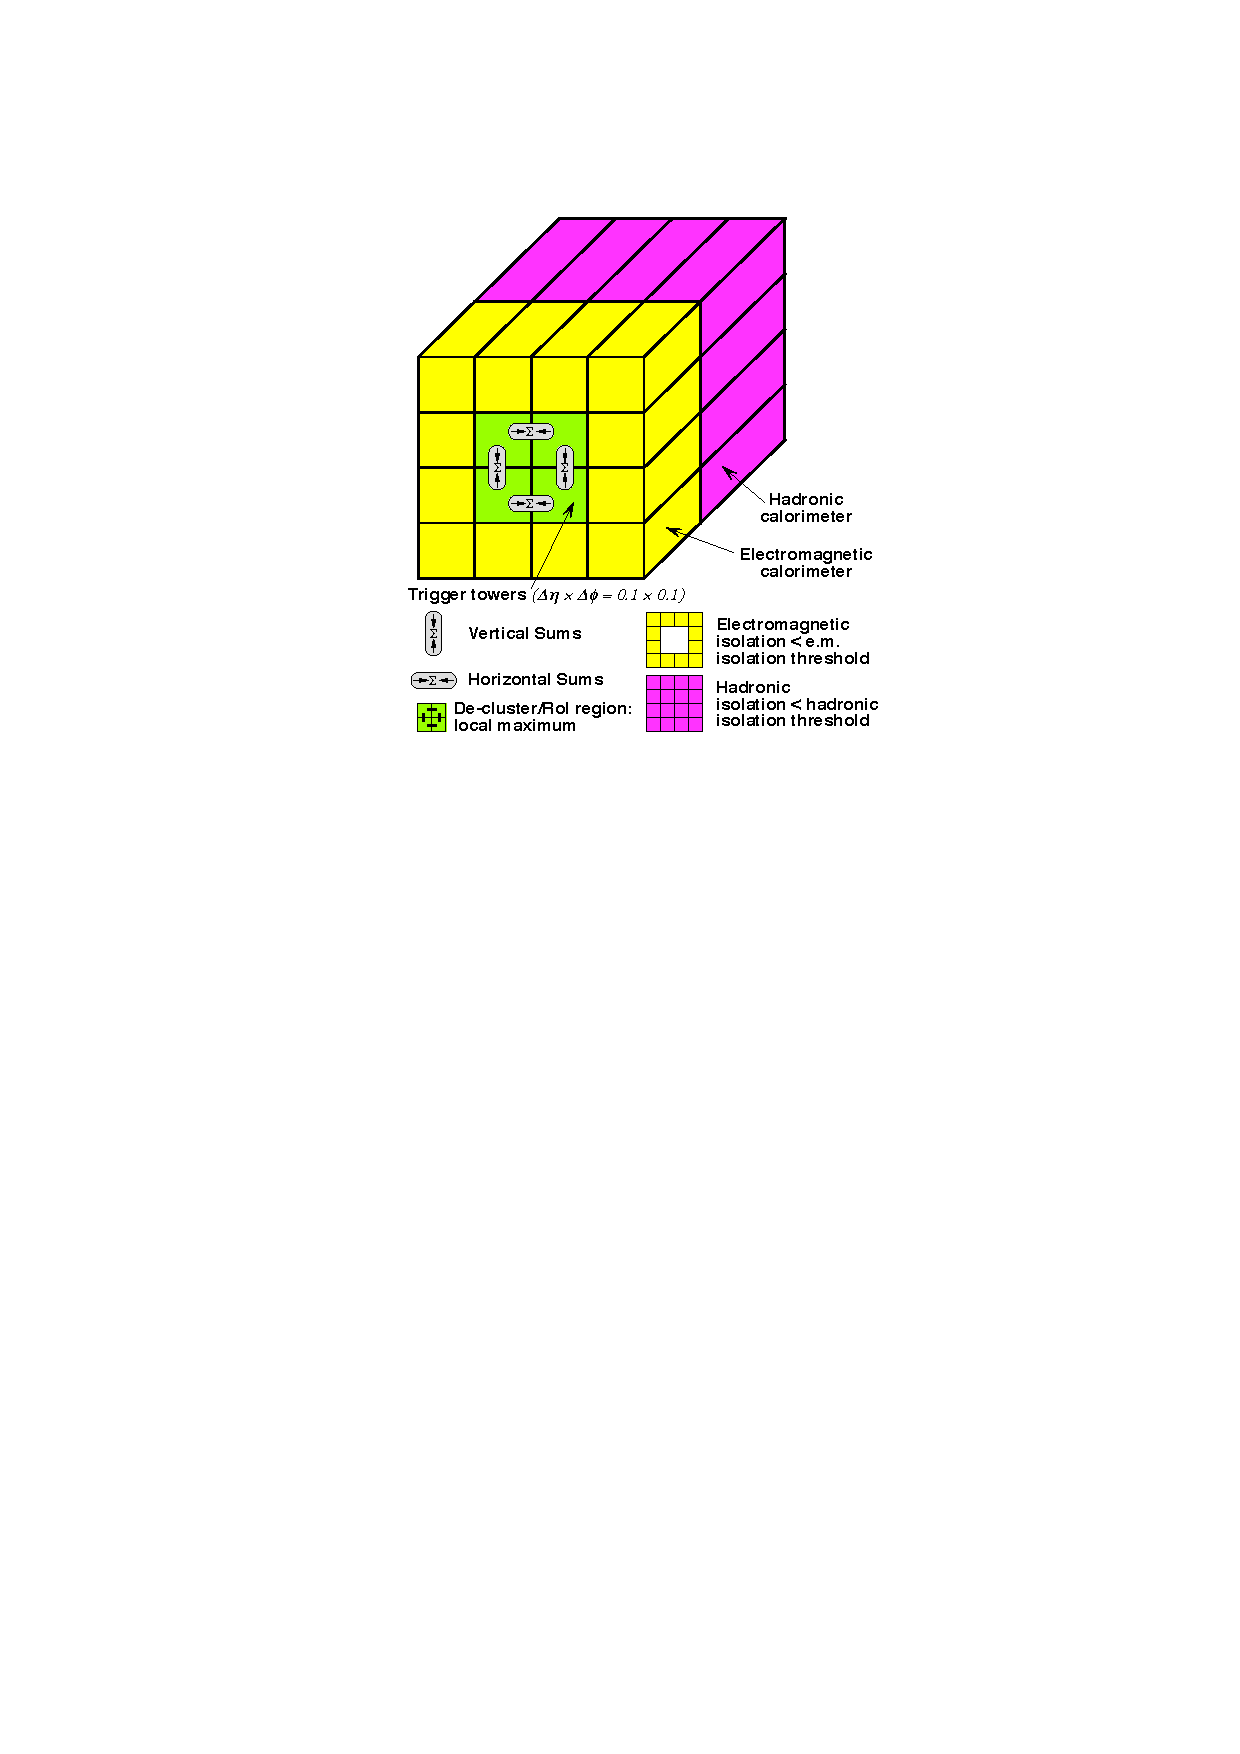
\includegraphics[width=0.4\textwidth]{figures/sliding_window_l1.pdf}
\caption[Torres de Trigger do primeiro nível de Trigger]{Torres de Trigger utilizadas para a seleção de elétrons no L1 do ATLAS. }
\label{fig:sliding_window_l1}
\end{figure}

\begin{itemize}
\item A soma das torres (EM e HAD) numa região $2\times2$ torres  em $\eta\times\phi$ localizadas no centro da janela de análise de L1: Esta hipótese é considerada bem sucedida caso o valor obtido com a soma das torres supere um determinado valor de corte.

\item $E_{T}$: quatro \textit{clusters}\footnote{um grupo de células que definem a região de interação da partícula com o calorímetro} eletromagnéticos sobrepostos, correspondendo a soma de duas torres. O \textit{cluster} mais energético deve ser maior ou igual a um determinado valor para o teste de hipótese ser bem sucedido. Este algoritmo determina a energia transversa da região analisada pelo L1.

\end{itemize}

O primeiro teste de hipótese serve apenas para determinar uma possível região de interesse (RoI). No caso de cortes sem isolamento, a região será aprovada somente se o segundo teste for bem sucedido. Para cortes com isolamento, a região de analise precisa ser aprovada por mais 4 testes de hipótese listados a seguir:

\begin{itemize}

\item $HAD_{Core}$ (Núcleo hadrônico): Soma das quatro torres do calorímetro hadrônico, posicionadas atrás dos \textit{clusters} eletromagnéticos.  Este teste será bem sucedido
caso esta soma seja menor ou igual a um dado patamar.

\item $EM_{Isol}$: Anel de isolamento eletromagnético, consistindo na soma da energia transversa das 12 torres eletromagnéticas posicionadas ao redor dos quatro 
\textit{clusters} eletromagnéticos. O teste é considerado aprovado caso o valor resultante da soma das 12 torres seja menor ou igual ao patamar de decisão estabelecido
para este corte.

\item $HAD_{Isol}$: Anel de isolamento hadrônico, correspondente à soma da energia transversa das 12 torres hadrônicas posicionadas ao redor do núcleo hadrônico.
O teste de hipotese será considerado aprovado caso o valor resultante da soma das 12 torres seja menor ou igual ao patamar de decisão estabelecido pelo corte.  

\end{itemize}

Dependendo da configuração requerida para o sistema de filtragem, os testes de hipótese acima serão aplicados sequencialmente. Caso seja aprovada,  a região de interesse do calorímetro será etiquetada e enviada para o sistema de filtragem de alto nível, onde novas extrações de características e algoritmos de hipótese mais sofisticados serão aplicados.

\subsection{Arquitetura do \textit{High Level Trigger}}

O sistema de \textit{Trigger} de alto nível recebe as regiões de interesse marcadas pelo nível 1 e realiza extrações de características e testes de hipóteses mais sofisticados, com granularidade
mais fina que seu nível anterior, para tomar a decisão de aceitação ou rejeição do evento. Neste nível, a latência é da ordem de milessegundos, o que possibilita a utilização de algoritmos mais
robustos e de maior custo computacional. Além das células do calorímetro, este nível utiliza a informação dos detectores de traço do ATLAS para compor a informação que será repassada para os testes de hipótese da configuração requerida para aceitação de um determinado padrão de evento na cadeia de \textit{Trigger}.

A arquitetura deste sistema foi implementada em software utilizando as linguagens C++, para compor o núcleo dos algoritmos, devido à necessidade de velocidade, e $python$
para a configuração e montagem da cadeia de execução do \textit{Trigger}, devido à sua simplicidade, fácil manutenção e adaptação.  Além disso, o atual sistema deve respeitar dois conceitos
bastante distintos que são utilizados em sequência para reduzir a taxa de eventos ao longo da cadeia de \textit{Trigger}.  Em outras palavras, este sistema é dividido em dois subsistemas: O sistema de \textit{Trigger} rápido (\textit{Fast}), o antigo L2, e o de alta precisão (\textit{Precision}), antigamente chamado de EF.  A Figura~\ref{fig:egammaChain} mostra o esquema de execução do \textit{Trigger} de alto nível para o canal $e/\gamma$. 

 
\begin{figure}[h!t]
\centering
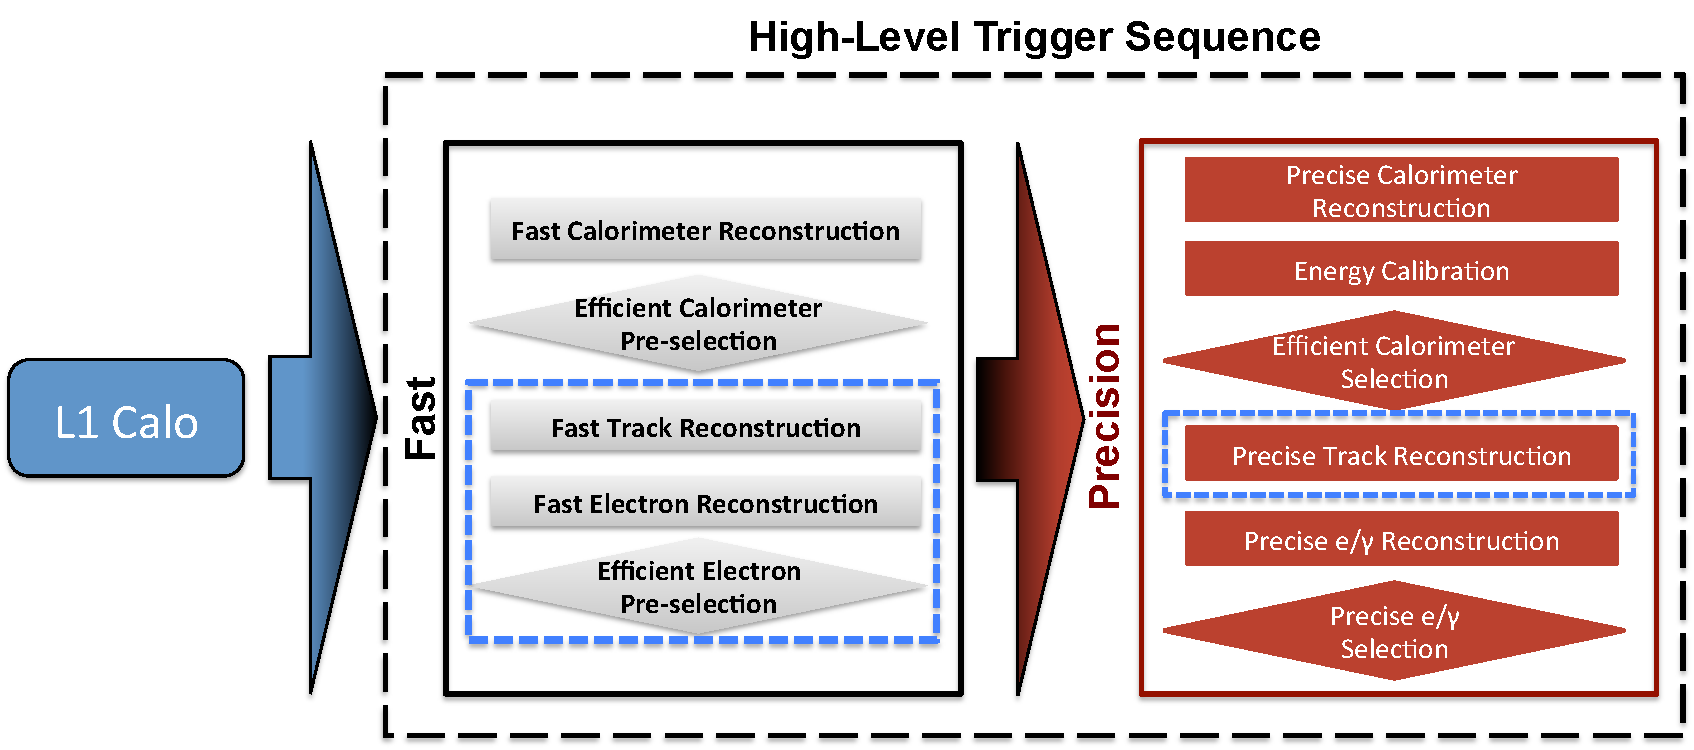
\includegraphics[width=0.8\textwidth]{figures/egammaChain.pdf}
\caption[Cadeia de execução dos algoritmos de \textit{trigger} do $e/\gamma$. ]
{Cadeia de execução dos algoritmos de extração de características (\textit{Reconstruction}), calibração e de testes de hipótese (\textit{Pre-selection} ou \textit{Selection}) para uma
configuração do $e/\gamma$. Extraído de \cite{artigo_acat2016_joao}.}
\label{fig:egammaChain}
\end{figure}

\subsubsection{Reconstrução Rápida do Calorímetro (\textit{Fast Calorimeter Reconstruction})}

Após receber a informação da RoI aceita pelo nível 1 com uma taxa de $\sim$100$k$Hz, o sistema de \textit{Trigger} rápido executa a reconstrução e extração de características do calorímetro com 
maior resolução utilizando um algoritmo para reconstrução de elétrons ou fótons baseado nas informações do chuveiro chamado de L2Calo. Esse, por sua vez, é uma versão limitada do algoritmo 
implementado na reconstrução precisa do calorímetro, devido à menor latência deste nível. A primeira etapa do L2Calo é refinar a posição em $\eta\times\phi$ da RoI, através do cálculo do 
baricentro da mesma, empregando, para tal, as células da segunda camada do calorímetro eletromagnético em sua granularidade mais fina. Em seguida, o L2Calo analisa
a energia e o perfil lateral e longitudinal do chuveiro produzido, resumindo esta informação em 4 variáveis. Estas variáveis são:

\begin{itemize}

\item Razão do Núcleo ($R_{core}$): Para a $2^{a}$ camada eletromagnética, $R_{core} = E_{3\times7}/E_{7\times7}$, onde $E_{m\times n}$ é a energia depositada em uma
região de $m\times n$ células em $\eta\times\phi$ ao redor da célula quente desta camada.

\item Razão de Energia ($E_{ratio}$): Para a $1^{a}$ camada eletromagnética, $E_{ratio} = (E_{1}-E_{2})/(E_{1}+E_{2})$, calculada em uma região de 
$\Delta\eta\times\Delta\phi = 0,125\times0,2$ ao redor do baricentro da RoI. $E_{1}$ e $E_{2}$ são, respectivamente, a primeira e a segunda célula
de maior energia.

\item Energia Transversa Eletromagnética ($E_{T_{EM}}$): É a energia transversa total depositada, nas 3 camadas eletromagnéticas, em uma região de 
$3\times7$ células em $\eta\times\phi$, centrada na célula quente da $2^{a}$ camada eletromagnética.
 
\item Razão de Energia Eletromagnética e Hadrônica ($E_{HAD}/E_{EM}$): $E_{HAD}$ é a energia transversa total depositada, nas 3 camadas hadrônicas, em 
uma janela de $\Delta\eta\times\Delta\phi=0, 2\times0, 2$ centrada no baricentro da RoI. 

\end{itemize}

\subsubsection{Seleção Eficiente do Calorímetro (\textit{Efficient Calorimeter Pre-selection})}

A próxima etapa da cadeia de \textit{Trigger} será aplicar o algoritmo de hipótese baseado nas variáveis de calorimetria extraídas da etapa de reconstrução rápida. O atual
algoritmo, chamado de T2Calo, realiza cortes lineares para cada uma das variáveis citadas anteriormente. Esses cortes são ajustados dependendo da assinatura requerida
pelo menu de \textit{Trigger} usado pela colaboração no momento da colisão ou simulação. O objetivo deste discriminador é reduzir a taxa de eventos utilizando somente
as células do calorímetro diminuindo assim o número de vezes que o algoritmo de traço, cujo custo computacional é mais alto, será executado na próxima etapa. 

\subsubsection{Reconstrução do traço e Pré-seleção de Elétrons (\textit{Fast Track Reconstruction and Efficient Electron Pre-selection})}

Nesta última etapa do \textit{Trigger} rápido os eventos aprovados pelo discriminador anterior executarão a reconstrução do traço utilizando o \gls{ftk}.
O \gls{ftk} é um sistema implementado em \gls{fpga} que recebe um conjunto de pontos do detector de  traço e, por meio de reconhecimento de padrão, retorna 
a trajetória da partícula caso, de fato, esses pontos definam uma trajetória.  Nessa etapa é computado o número de pontos ativados no detector de traço e o $p_{T}$. Então, o algoritmo de reconstrução de elétrons, chamado de L2Electron,  acessa essas informações e combina-as com as de calorimetria para usá-las na tomada de 
decisão na fase de teste de hipótese. Por fim, essa tomada de decisão é chamada de passo eficiente de pré-seleção de elétrons (\textit{Efficient Electron Pre-selection}).

\subsubsection{Reconstrução Precisa do Calorímetro, Calibração e Seleção Eficiente do Calorímetro}

Toda a infraestrutura que descreve o evento físico, no caso o objeto $e/\gamma$, na etapa precisa do \textit{Trigger} foi implementada de forma idêntica ao sistema de filtragem  \textit{offline}. 
Os algoritmos de reconstrução e os de hipóteses também foram idealizados de forma parecida porém de forma degradada devido aos requisitos de latência do sistema \textit{online}.  
Após receber os eventos aprovados no \textit{Trigger} na etapa anterior, a reconstrução do calorímetro é feita utilizando um algoritmo baseado nas informações do chuveiro da partícula
semelhante ao utilizado no L2Calo. No entanto,  esse possui uma maior complexidade e sofisticação na construção das variáveis devido aos algoritmos de ajuste e correções de energias
aplicados pela calibração nesta etapa, o que produz uma informação mais precisa e completa sobre a interação do evento com o calorímetro.

No teste de hipótese aplicado sobre os eventos desta etapa, pode-se escolher, atualmente, dois tipos de discriminadores configurados para atender a assinatura de  \textit{Trigger} requerida 
no momento da execução da cadeia de \textit{Trigger}. O primeiro deles é o T2Calo, que realiza os cortes lineares sobre as variareis extraídas do calorímetro. A outra opção é utilizar 
um \textit{Naive Bayes} como discriminador para tomar a decisão final nesta etapa de calorimetria, o que realiza os testes de hipótese por máxima verossimilhança (\textit{Likelihood, LH}).



\subsubsection{Reconstrução do Traço, do $e/\gamma$ e Seleção Precisa de Eventos}

No último estágio do \textit{Trigger}, a informação gerada na reconstrução do traço, utilizando um algoritmo mais complexo, combinada com a precisa informação de calorimetria gerada na etapa anterior 
é utilizada como entrada no teste final de hipótese. Com tudo, dependendo da configuração da assinatura aplicada na cadeia de \textit{Trigger}, um dos dois testes de hipótese
citados anteriormente pode ser utilizado para realizar essa discriminação. Por fim, combinando todos os testes de hipóteses aplicados no  \textit{Trigger} de alto nível, a taxa de eventos 
produzidos sofre uma redução dos $\sim$100$k$Hz iniciais após o primeiro nível de filtragem, para uma saída de aproximadamente 1$k$Hz, dependendo da assinatura de \textit{Trigger} requerida. 

\subsection{Sistema de Filtragem \textit{Offline}}

Conforme explicado no início deste capítulo, para sistemas de filtragem \textit{online}, uma vez que um evento é rejeitado, não é possível recuperar o mesmo. Desta forma,
para evitar a perda de um canal físico relevante, a eficiência de detecção é aumentada, com o custo de aumentar, também, o falso alarme. Consequentemente, ao final de um sistema
de filtragem \textit{online} ainda se encontram eventos, provenientes de ruído de fundo, misturados com os canais de interesse. Adicionalmente, os dados armazenados serão destinados
a inúmeros estudos distintos (bóson de Higgs, supersimetria, etc.), onde cada estudo necessitará observar um determinado subgrupo de eventos armazenados após a filtragem \textit{online}.

Para atender ao seu uso bastante diversificado, sistemas de filtragem \textit{offline} são empregados. Neste modelo de filtragem, uma vez que o tempo de processamento
não é um fator crítico, algoritmos mais complexos e eficientes podem ser empregados para analisar cada evento, de acordo com os requisitos específicos ao estudo sendo conduzido. Normalmente,
técnicas baseadas na estimação da função de densidade de probabilidade (PDF) do sinal de interesse são exploradas. Métodos \textit{bayesianos} de análise são frequentemente utilizados para testar
a hipótese de ocorrência de um determinado canal físico. Hipóteses também podem ser testadas ao comparar-se se a PDF do canal físico desejado está similar à distribuição de probabilidade
descrita pela teoria para este canal por meio de simulação de Monte Carlo. 

\subsection{Assinaturas de \textit{Trigger} e seus Sufixos}

Uma assinatura, também chamadas de \textit{chain}, é um esquema de configuração onde o nome do \textit{Trigger} é mapeado em uma lista de configurações e cortes realizados pelo sistema
de montagem do Trigger. A Tabela~\ref{tab:egammaChains_exemplos} mostra o esquema de configuração do primeiro nível de \textit{Trigger}, dos algoritmos de extração de 
características, do inglés \textit{Feature Extraction} (FEX), e de hipótese, \textit{Hypothesis} (HYPO)  para cada uma das \textit{chains}.  
Em geral, as \textit{chains} possuem critérios de ajustes na taxa de detecção e seleções especiais embutidos em seu próprio nome. Dentre os principais sufixos encontrados nos nomes das 
assinaturas podemos citar: 

\begin{itemize}

\item $e(E_{T_{cut}}$) ou $g(E_{T_{cut}}$): Representam assinaturas de elétrons ($e$) ou fótons ($g$) com $E_{T} > E_{T_{cut}} GeV$. Exemplo: e5, e25, g25, etc.

\item \textit{loose}, \textit{medium} e \textit{tight}: Esses sufixos representam ajustes nos cortes realizados pelos discriminadores aplicados na etapa de hipótese no \textit{Trigger} de alto nivel utilizando 
o T2Calo como base. Em geral, um critério \textit{loose} representa uma maior aceitação no \textit{Trigger} utilizando critérios mais relaxados. Em consequência disso, uma maior taxa de detecção e 
falso alarme são esperados para essa configuração. No entanto, para o critério \textit{tight} a ideia é oposta. Neste caso, uma amostra mais pura de eventos é extraída do \textit{Trigger} utilizando cortes mais 
apertados produzindo assim uma taxa de falso alarme bastante reduzida. Por fim, o critério \textit{medium} realiza o balanço entre esses dois casos.

\item \textit{lhloose}, \textit{lhmedium} e \textit{lhtight}: Representam a mesma ideia dos critérios acima porém utilizam a \textit{likelihood} como algoritmo de hipótese.

\item \textit{etcut}: O único corte aplicado nos algoritmos de hipótese é o de $E_{T}$ maior que um determinado valor em GeV;

\item \textit{iloose}: Exigência de evento isolado requerida para o \textit{Trigger}.

\end{itemize}

\begin{landscape}
% Please add the following required packages to your document preamble:
% \usepackage{multirow}
\begin{table}[p]\scriptsize
\centering
\begin{tabular}{ccccccccccc}
\hline
\hline
\multirow{4}{*}{\textit{\textbf{Chain}}} & \textbf{L1Calo} & \multicolumn{8}{c}{\textbf{HLT (\textit{High Level Trigger})}} & \multirow{4}{*}{\textbf{\begin{tabular}[c]{@{}c@{}}Ajuste \\ do corte\end{tabular}}} \\ \cline{3-10}
 &  & \multicolumn{4}{c}{\textit{\textbf{Fast}}} & \multicolumn{4}{c}{\textbf{Precision}} &  \\ \cline{3-10}
 &  & \multicolumn{2}{c}{\textbf{Calo}} & \multicolumn{2}{c}{\textbf{Electron}} & \multicolumn{2}{c}{\textbf{Calo}} & \multicolumn{2}{c}{\textbf{$e/\gamma$}} &  \\ \cline{3-10}
 &  & FEX & HYPO & FEX & HYPO & FEX & HYPO & FEX & HYPO &  \\ \hline
e24\_medium\_L1EM18VH & $E_{T} > 18GeV$ & Shower & T2Calo & \begin{tabular}[c]{@{}c@{}}FTK\\ +Shower\end{tabular} & \begin{tabular}[c]{@{}c@{}}T2Calo\\ Combined\end{tabular} & Shower & T2Calo & \begin{tabular}[c]{@{}c@{}}Shower\\ +Tracker\\ +Calibration\end{tabular} & \begin{tabular}[c]{@{}c@{}}T2Calo\\ Combined\end{tabular} & medium \\ \hline
e24\_lhmedium\_nod0\_iloose & \begin{tabular}[c]{@{}c@{}}$E_{T} > 20GeV$\\ Isolated\end{tabular} & Shower & T2Calo & \begin{tabular}[c]{@{}c@{}}FTK\\ +Shower\end{tabular} & \begin{tabular}[c]{@{}c@{}}T2Calo\\ Combined\end{tabular} & Shower & Likelihood & \begin{tabular}[c]{@{}c@{}}Shower\\ +Tracker\\ +Calibration\end{tabular} & \begin{tabular}[c]{@{}c@{}}Likelihood\\ Isolated\end{tabular} & medium \\ \hline
e24\_tight\_L1EM22VHI & \begin{tabular}[c]{@{}c@{}}$E_{T} > 22GeV$\\ Isolated\end{tabular} & Shower & T2Calo & \begin{tabular}[c]{@{}c@{}}FTK\\ +Shower\end{tabular} & \begin{tabular}[c]{@{}c@{}}T2Calo\\ Combined\end{tabular} & Shower & T2Calo & \begin{tabular}[c]{@{}c@{}}Shower\\ +Tracker\\ +Calibration\end{tabular} & T2Calo & tight \\ \hline
e5\_etcut & $E_{T} > 3GeV$ & Shower & No Cut & \begin{tabular}[c]{@{}c@{}}FTK\\ +Shower\end{tabular} & No Cut & Shower & $E_{T}$ \textgreater 5GeV & \begin{tabular}[c]{@{}c@{}}Shower\\ +Tracker\\ +Calibration\end{tabular} & No Cut &  \\ \hline \hline
\end{tabular}
\centering

\caption[Descrição de algumas assinaturas aplicadas no \textit{Trigger}]
{Descrição das configurações de \textit{Trigger} para cada uma das  \textit{chains}.  Os cortes em energia para o nível 1 estão representados na coluna 
do L1Calo. Cada posição do HLT foi preenchida com o nome do respectivo algoritmo para sua \gls{fex} e \gls{hypo} respectivamente. }

\label{tab:egammaChains_exemplos}
\end{table}

\end{landscape}





\chapter{\textit{Neural Ringer}: Alternativa de \textit{Trigger}}
\label{cap:metodologia}
\glsresetall

Em problemas de filtragem \textit{online} onde diferentes níveis de \textit{trigger} implementados de forma hierárquica, do sistema mais simples
ao mais robusto, é sempre atraente otimizar os primeiros níveis dessa cadeia. Uma vez que, ao se aumentar a eficiência de detecção
e a rejeição a eventos não interessantes para o estudo, diminui-se o número de vezes em que os sistemas de filtragem superiores,
muitas vezes de maior latência, sejam utilizados com eventos que claramente não são necessários para o estudo de interesse.

Em outras palavras é desejado que eventos que seriam eliminados em sistemas de filtragem mais complexos como os níveis 
hierárquicos superiores sejam eliminados pelos níveis inferiores. Assim, esses sistemas mais complexos somente se encarregariam
de eventos que sejam realmente necessário a utilização de algoritmos e ferramentas mais complexas para efetuar sua discriminação.

O foco deste trabalho será na otimização do sistema de filtragem \textit{online} de alto nível do ATLAS na etapa de Calorimetria do \textit{Trigger} rápido.
Aqui, será implementado um novo algoritmo de extração de característica e também um novo algoritmo de hipótese baseado em redes neurais artificiais 
do tipo \gls{mlp}, na etapa de pre-seleção eficiente do calorímetro.

\newpage
\section{O Neural \textit{Ringer}}

O Neural \textit{Ringer} é um algoritmo que combina extração de características e o teste de hipótese para a discriminação de elétrons no \textit{trigger} de decisão rápida na etapa
de calorimetria. Toda as estrutura da nova extração de características foi implementada sobre a propria infraestrutura do algoritmo padrão utilizado pelo \textit{trigger} dentro
do \textit{framework} do
\textit{Athena}\footnote{É um \textit{framework} baseado em C++ e \textit{Python} utilizado pela colaboração para executar e testar todas as ferramentas de simulação e 
análise de eventos. Nesta ferramenta, também está integrada a implementação do sistema \textit{online} e \textit{offline} do detector \gls{atlas}, assim como o 
monitoramento de todos os sistemas do detector.}
, possibilitando, assim, o compartilhamento de informações entre os dois algoritmos e preservando o legado de código já existente no sistema.


\subsection{Algoritmo de Extração de Características (FEX)}

O \textit{FastCaloRinger} é um algoritmo extração de características alternativo do $e/\gamma$. A informação de calorimetria das regiões de interesse selecionadas pelo L1 é 
compactada na forma de anéis concêntricos de deposição de energia. Todas as células de deposição de energia dos calorímetros eletromagnético e hadrônico, dentro da RoI, são utilizadas. 
Primeiramente, o algoritmo procura pela célula mais energética da segunda camada eletromagnética. Essa célula forma o primeiro anel. A energia das células vizinhas ao primeiro anel são somadas, 
formando a energia do segundo anel. 

Esse processo é repetido até que todas as células da região de interesse sejam utilizadas (ou um número máximo de anéis seja alcançado). Esse processo é 
repetido em todas as camadas dos calorímetros, utilizando a posição da célula mais energética da segunda camada eletromagnética como referência para o primeiro anel das outras camadas. 
A Figura~\ref{fig:ringer_sketch} ilustra a configuração de anéis para diferentes camadas dos calorímetros. Esse mapeamento em anéis concêntricos preserva as características de deposição de 
energia de elétrons e jatos, contribuindo, assim, para a discriminação dessas partículas.

\begin{figure}[h!t]
\centering
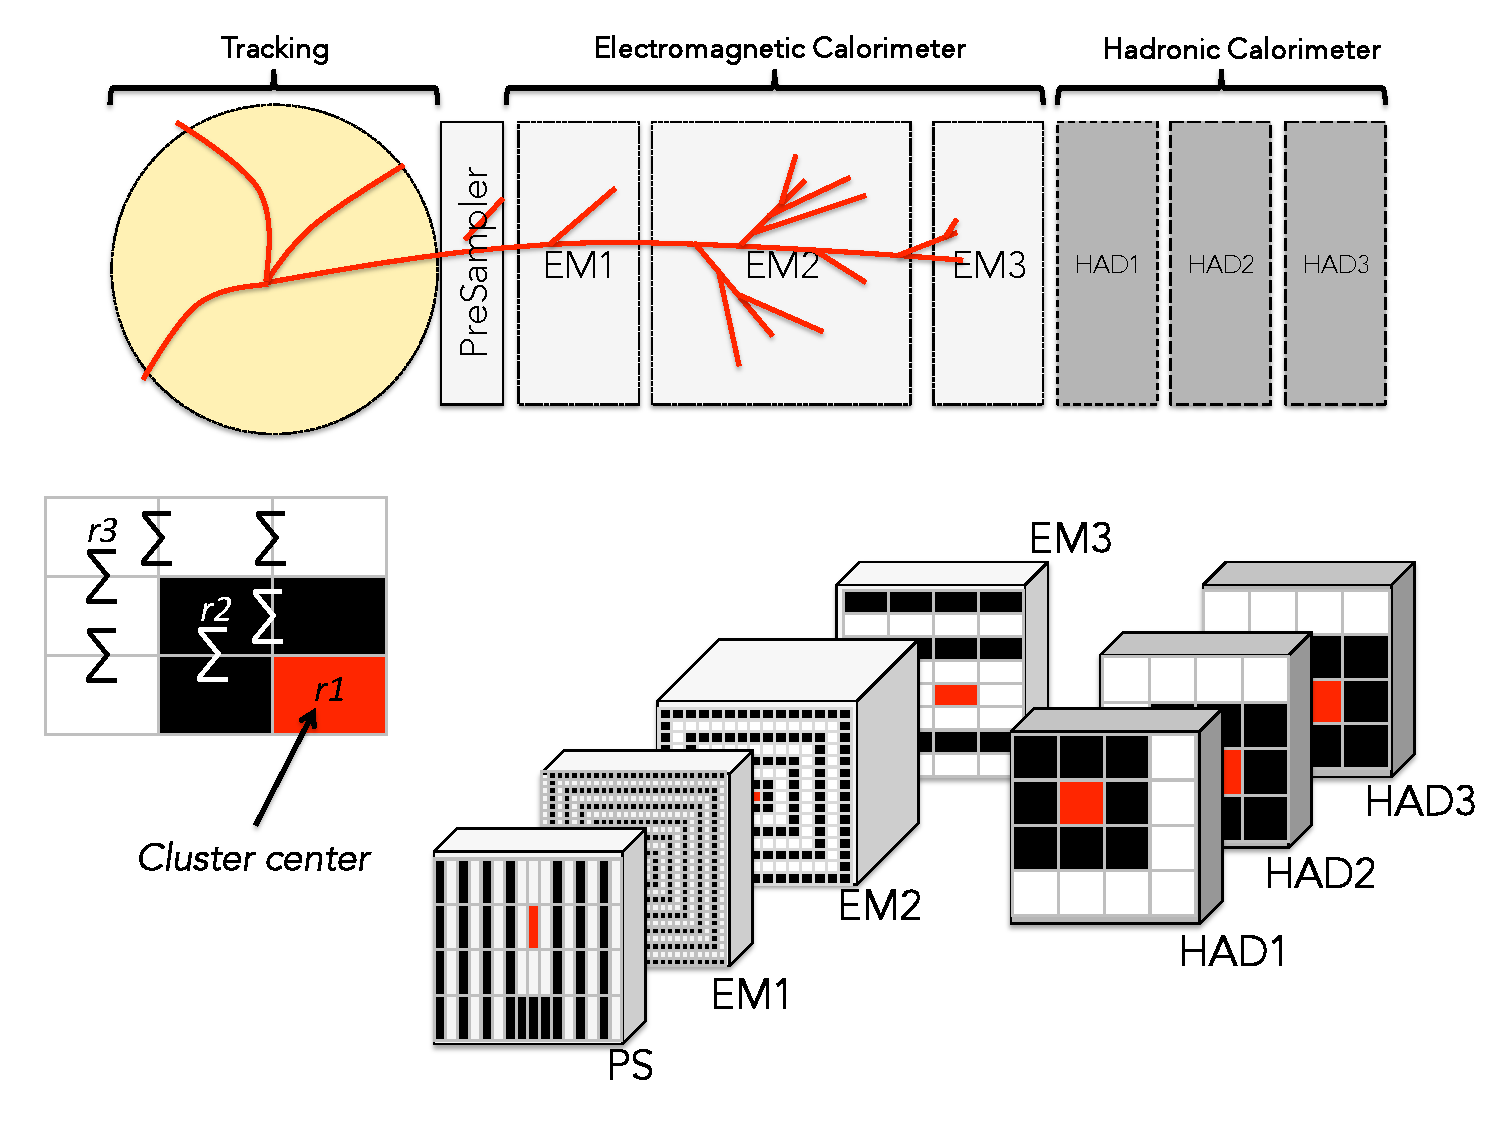
\includegraphics[width=0.8\textwidth]{figures/ringerAlgorithmSketch.pdf}
\caption[Visão simplificada da montagem dos anéis utilizada pelo algoritmo de extração de características.]{Visão simplificada da montagem dos anéis 
utilizada pelo algoritmo de extração de características proposto para cada uma das camadas dos calorímetros.}
\label{fig:ringer_sketch}
\end{figure}

No total, cem anéis são extraídos das sete camadas dos calorímetros. Cada camada tem um número próprio de anéis, de acordo com a sua granularidade. O número de anéis
para cada camada está representado na Tabela~\ref{tab:aneis_por_camada}.


\begin{table}[h]
\centering
\resizebox{\textwidth}{!}{%
\begin{tabular}{cccccccc}
\hline
\hline
\multirow{2}{*}{Camada} & \multicolumn{4}{c}{Calorímetro Eletromagnético} & \multicolumn{3}{c}{Calorímetro Hadrônico} \\ \cline{2-8} 
 & Pre-Sampler & EM.1 & EM.2 & EM.3 & HAD.1 & HAD.2 & HAD.3 \\ \hline
\#anéis & 8 & 64 & 8 & 8 & 4 & 4 & 4 \\ \hline \hline
\end{tabular}%
}
\caption[Número de anéis extraídos em cada camada dos calorímetros]{Número de anéis extraídos para cada uma das camadas dos calorímetros
eletromagnético e hadrônico do \gls{atlas}.}
\label{tab:aneis_por_camada}
\end{table}

\subsection{Algoritmo de Hipótese (HYPO)}

Complementar à nova proposta de extração de características dos calorímetros, também foi desenvolvida uma nova abordagem de
hipótese utilizando uma rede neural artificial  \gls{mlp} como classificador. Esse classificador neural foi implementado na infraestrutura
do \textit{trigger} de forma a ser alimentado pelos anéis do algoritmo de extração. Por definição, a estrutura utilizada é formada 
por cem entradas, uma camada escondida, cujo o número de neurônios é determinado empiricamente pelo método
de treinamento, e apenas um neurônio na camada de saída. A função de ativação de todos os neurônios é a tangente hiperbólica.
A Figura~\ref{fig:topologia_rna} representa uma estrutura genérica de uma rede neural artificial do tipo multi-camada.

\begin{figure}[h!t]
\centering
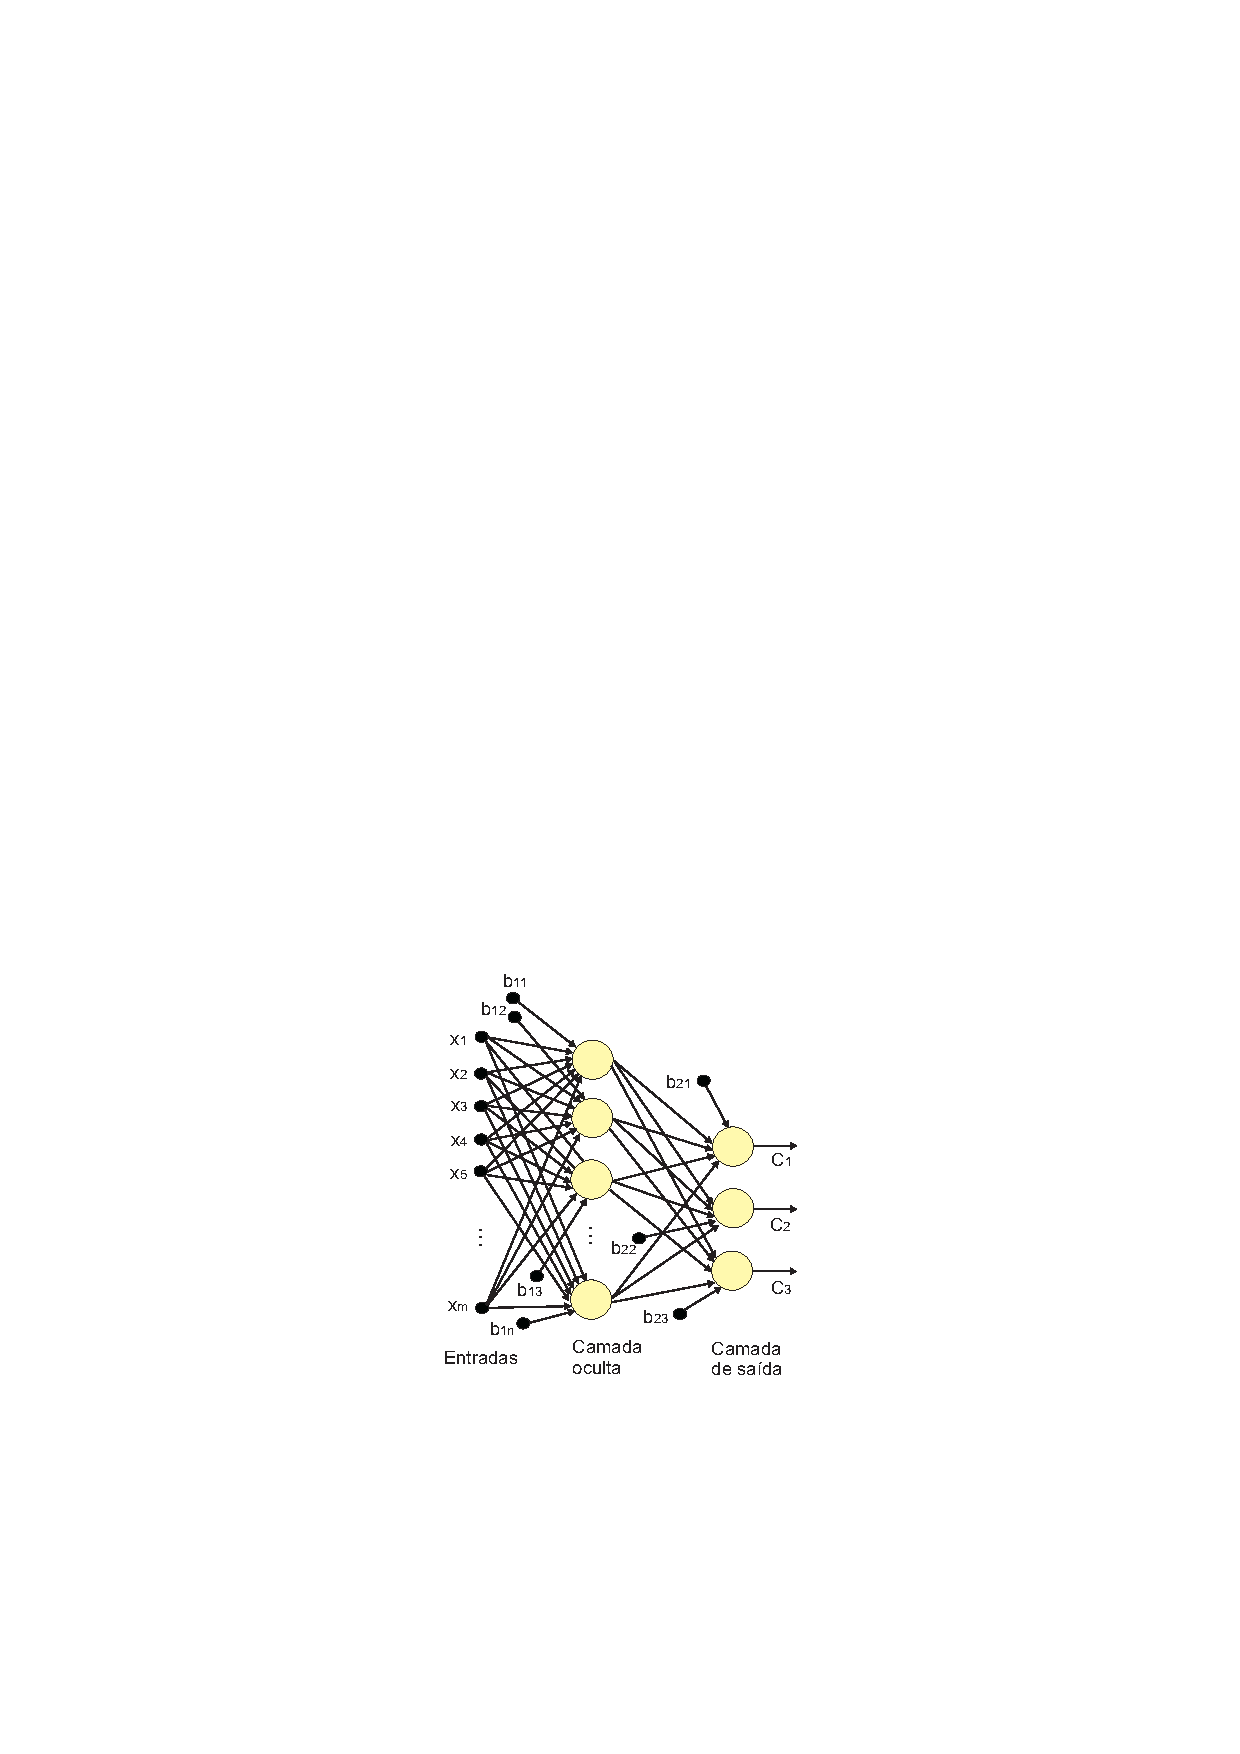
\includegraphics[width=0.4\textwidth]{figures/topologia_rna.pdf}
\caption[Representação da estrutura de uma rede neural do tipo multicamada.]
{Representação da estrutura de uma rede neural do tipo multi-camada, genérica, com apenas uma camada escondida.}
\label{fig:topologia_rna}
\end{figure}

O algoritmo recebe os anéis e realiza um tipo de pré-processamento (o padrão é a normalização de cada anel pela energia total dos anéis)
e repassa essa informação para uma rede neural artificial previamente treinada. Por fim, a saída da rede é comparada com um limiar de corte
que é ajustado dependendo da configuração da \textit{chain} a ser executada pelo \textit{trigger}.

\subsection{Proposta de Assinatura}

Foi selecionada como referência para o treinamento do classificador uma das assinaturas responsáveis pela 
identificação dos elétrons pertencentes ao decaimento $H\rightarrow ZZ\rightarrow 4e$. Assim, o \textit{Neural Ringer}
será comparado com a respectiva etapa de trigger da \textit{chain} de referência escolhida

A otimização do sistema de \textit{trigger} será implementada conforme mostrado na Tabela~\ref{tab:chain_do_ringer}, onde o algoritmo de extração do \textit{ringer},
combinado com a hipótese baseada em um classificado \gls{mlp}, estão localizados na primeira etapa de calorimetria do \textit{trigger} de alto nível.  Assim, uma nova \textit{chain} 
foi criada utilizando o sufixo \textit{ringer} para indicar no \textit{menu} de \textit{trigger} a utilização do algoritmo alternativo \textit{Neural Ringer} na cadeia de filtragem. A assinatura
utilizada como referência também está representada nesta tabela.



\begin{landscape}

% Please add the following required packages to your document preamble:
% \usepackage{multirow}
% \usepackage[table,xcdraw]{xcolor}
% If you use beamer only pass "xcolor=table" option, i.e. \documentclass[xcolor=table]{beamer}
\begin{table}[p]\scriptsize
\centering
\begin{tabular}{ccccccccccc}
\hline
\hline
 & \textbf{L1Calo} & \multicolumn{8}{c}{HLT \textit{\textbf{(High Level Trigger)}}} &  \\ \cline{3-10}
 &  & \multicolumn{4}{c}{{\color[HTML]{333333} \textit{\textbf{Fast}}}} & \multicolumn{4}{c}{{\color[HTML]{000000} \textbf{Precision}}} &  \\ \cline{3-10}
 &  & \multicolumn{2}{c}{{\color[HTML]{333333} \textbf{Calo}}} & \multicolumn{2}{c}{{\color[HTML]{333333} \textbf{Electron}}} & \multicolumn{2}{c}{{\color[HTML]{000000} \textbf{Calo}}} & \multicolumn{2}{c}{{\color[HTML]{000000} \textbf{$e/\gamma$}}} &  \\ \cline{3-10}
\multirow{-4}{*}{\textit{\textbf{Chain}}} &  & {\color[HTML]{FE0000} \textbf{FEX}} & {\color[HTML]{FE0000} \textbf{HYPO}} & {\color[HTML]{333333} FEX} & {\color[HTML]{333333} HYPO} & {\color[HTML]{000000} FEX} & {\color[HTML]{000000} HYPO} & {\color[HTML]{000000} FEX} & {\color[HTML]{000000} HYPO} & \multirow{-4}{*}{\textbf{\begin{tabular}[c]{@{}c@{}}Ajuste \\ do corte\end{tabular}}} \\ \hline
\begin{tabular}[c]{@{}c@{}}e24\_lhmedium\_nod0\_ringer\_iloose\\ (Proposta do Trabalho)\end{tabular} & \begin{tabular}[c]{@{}c@{}}$E_{T} > 20GeV$\\ \\ Isolated\end{tabular} & {\color[HTML]{FE0000} \textbf{Ringer}} & {\color[HTML]{FE0000} \textbf{\begin{tabular}[c]{@{}c@{}}Neural\\ Network\end{tabular}}} & {\color[HTML]{333333} \begin{tabular}[c]{@{}c@{}}FTK\\ +Shower\end{tabular}} & {\color[HTML]{333333} \begin{tabular}[c]{@{}c@{}}T2Calo\\ Combined\end{tabular}} & {\color[HTML]{000000} Shower} & {\color[HTML]{000000} Likelihood} & {\color[HTML]{000000} \begin{tabular}[c]{@{}c@{}}Shower\\ +Tracker\\ +Calibration\end{tabular}} & {\color[HTML]{000000} \begin{tabular}[c]{@{}c@{}}Likelihood\\ Combined\end{tabular}} & medium \\ \hline
\begin{tabular}[c]{@{}c@{}}e24\_lhmedium\_nod0\_iloose\\ (Referência)\end{tabular} & \begin{tabular}[c]{@{}c@{}}$E_{T} > 20GeV$\\ Isolated\end{tabular} & {\color[HTML]{FE0000} \textbf{Shower}} & {\color[HTML]{FE0000} \textbf{T2Calo}} & {\color[HTML]{333333} \begin{tabular}[c]{@{}c@{}}FTK\\ +Shower\end{tabular}} & {\color[HTML]{333333} \begin{tabular}[c]{@{}c@{}}T2Calo\\ Combined\end{tabular}} & {\color[HTML]{000000} Shower} & {\color[HTML]{000000} Likelihood} & {\color[HTML]{000000} \begin{tabular}[c]{@{}c@{}}Shower\\ +Tracker\\ +Calibration\end{tabular}} & {\color[HTML]{000000} \begin{tabular}[c]{@{}c@{}}Likelihood\\ Isolated\end{tabular}} & medium \\
\hline
\hline
\end{tabular}


\caption[Representação do fluxo de algoritmos e cortes realizados para a \textit{chain} do \textit{ringer} e a referência.]
{Representação do fluxo de algoritmos e cortes realizados para a \textit{chain} do \textit{ringer} e a referência. As colunas em vermelho representam as etapas do \textit{trigger} que serão otimizadas.}
\label{tab:chain_do_ringer}
\end{table}

\end{landscape}


\section{Método}

O algoritmo de extração de características do \textit{Neural Ringer} fornece os anéis necessários para a descrição do perfil de deposição de energia da RoI para o \textit{trigger} de alto nível.
O algoritmo de hipótese, baseado numa rede neural, deve operar sobre esses anéis para fornecer a decisão da \textit{chain}. Entretanto, para o treinamento supervisionado
da rede neural, cada RoI deve ser previamente etiquetada de acordo com a sua natureza. No caso de simulações de Monte Carlo, essa informação é feita de acordo 
com a informação da \textit{truth} ou da decisão das análises realizadas pelo \textit{offline}. 

\subsection{Conjunto de Dados}

Os estudos do algoritmo proposto foram realizados utilizando simulações de Monte Carlo de 2014, que contemplam um cenário de operação de energia
envolvida de 13 $TeV$. Nessas condições, a quantidade de empilhamento de eventos é considerável. Na simulação, podem haver, em média, até 20 colisões  
inelásticas. Entretanto, se essas interações ocorrem em uma mesma região do detector, a esse efeito dar-se o nome de empilhamento, a informação sobreposta 
pode impedir a correta identificação das partículas.

Utilizam-se simulações de Monte Carlo para a produção de bósons $Z$ com os algoritmos de hipótese mais atuais e assinaturas \textit{trigger} para a identificação
de elétrons decorrentes do decaimento $Z\rightarrow ee$. Como ruído de fundo do processo de decaimento do bóson $Z$, utilizaram-se simulações de jatos com energia
concentrada em 17 $GeV$, operando sobre as mesmas condições já descritas. As simulações alimentam os emuladores dos sistemas do \gls{atlas} (através do
\textit{framework} do \textit{Athena}), fornecendo uma resposta similar àquela observada experimentalmente.

\subsection{Seleção de Sinais}
\label{sec:selecao_sinais}
As RoI de todos os dados utilizados na simulação de Monte Carlo devem ser classificadas antes da fase de treinamento dos
discriminadores . Assim para a seleção dos elétrons foi utilizada uma abordagem baseada na resposta das análises \textit{offline}. Porém
para o conjunto que irá formar o ruído de fundo, no caso os jatos, será utilizada uma abordagem baseada na natureza da partícula
dada pela própria simulação (\textit{truth}). Os critérios utilizados para a seleção dos eventos para a construção da \textit{chain} proposta são:

\begin{description}
\item[Seleção dos elétrons]: Todas as RoI selecionadas pelo L1 nos dados simulados para o decaimento $Z\rightarrow ee$ são casadas com 
os objetos reconstruídos no ambiente \textit{offline}, através de suas posições $\eta\times\phi$. Posteriormente, um corte de $E_{T}>19GeV$ é aplicado nos \textit{clusters} formados pelo
sistema de calorimetria rápida do \textit{trigger} de alto nível. Por fim, uma RoI é considerada como elétron caso o seu objeto \textit{offline} associado tenha sido aprovado pelo critério \textit{tight} utilizado 
pelo algoritmo de hipótese configurado para esta \textit{chain}.

\item[Seleção dos jatos]: Todas as RoI selecionadas pelo L1 nos dados simulados para os jatos são casadas com seus objetos \textit{truth}, através de suas posições $\eta\times\phi$. 
Posteriormente, um corte de $E_{T}>19GeV$ é aplicado nos \textit{clusters} formados pelo sistema de calorimetria rápida do \textit{trigger} de alto nível. Por fim, uma RoI é considerada 
jato caso sua natureza não seja a de um elétron pela simulação de Monte Carlo.

\end{description}

%A Figura~\ref{fig:perfil_ringer} representa o perfil médio energético, medido em $MeV$, dos anéis para as amostras de elétrons do conjunto de $Z\rightarrow ee$ e de partículas hadrônicas pertencentes 
%ao conjunto de jatos em $E_{T}>17 GeV$. Comparando os dois perfis de energia observa-se que as partículas hadrônicas excitam os anéis mais externos de cada camada além de liberar, em média, 
%mais energia na camada hadrônica. Assim, os jatos possuem um chuveiro mais largo e profundo que as interações dos elétrons no calorímetro. 

%\begin{figure}[h!t]
%\centering
%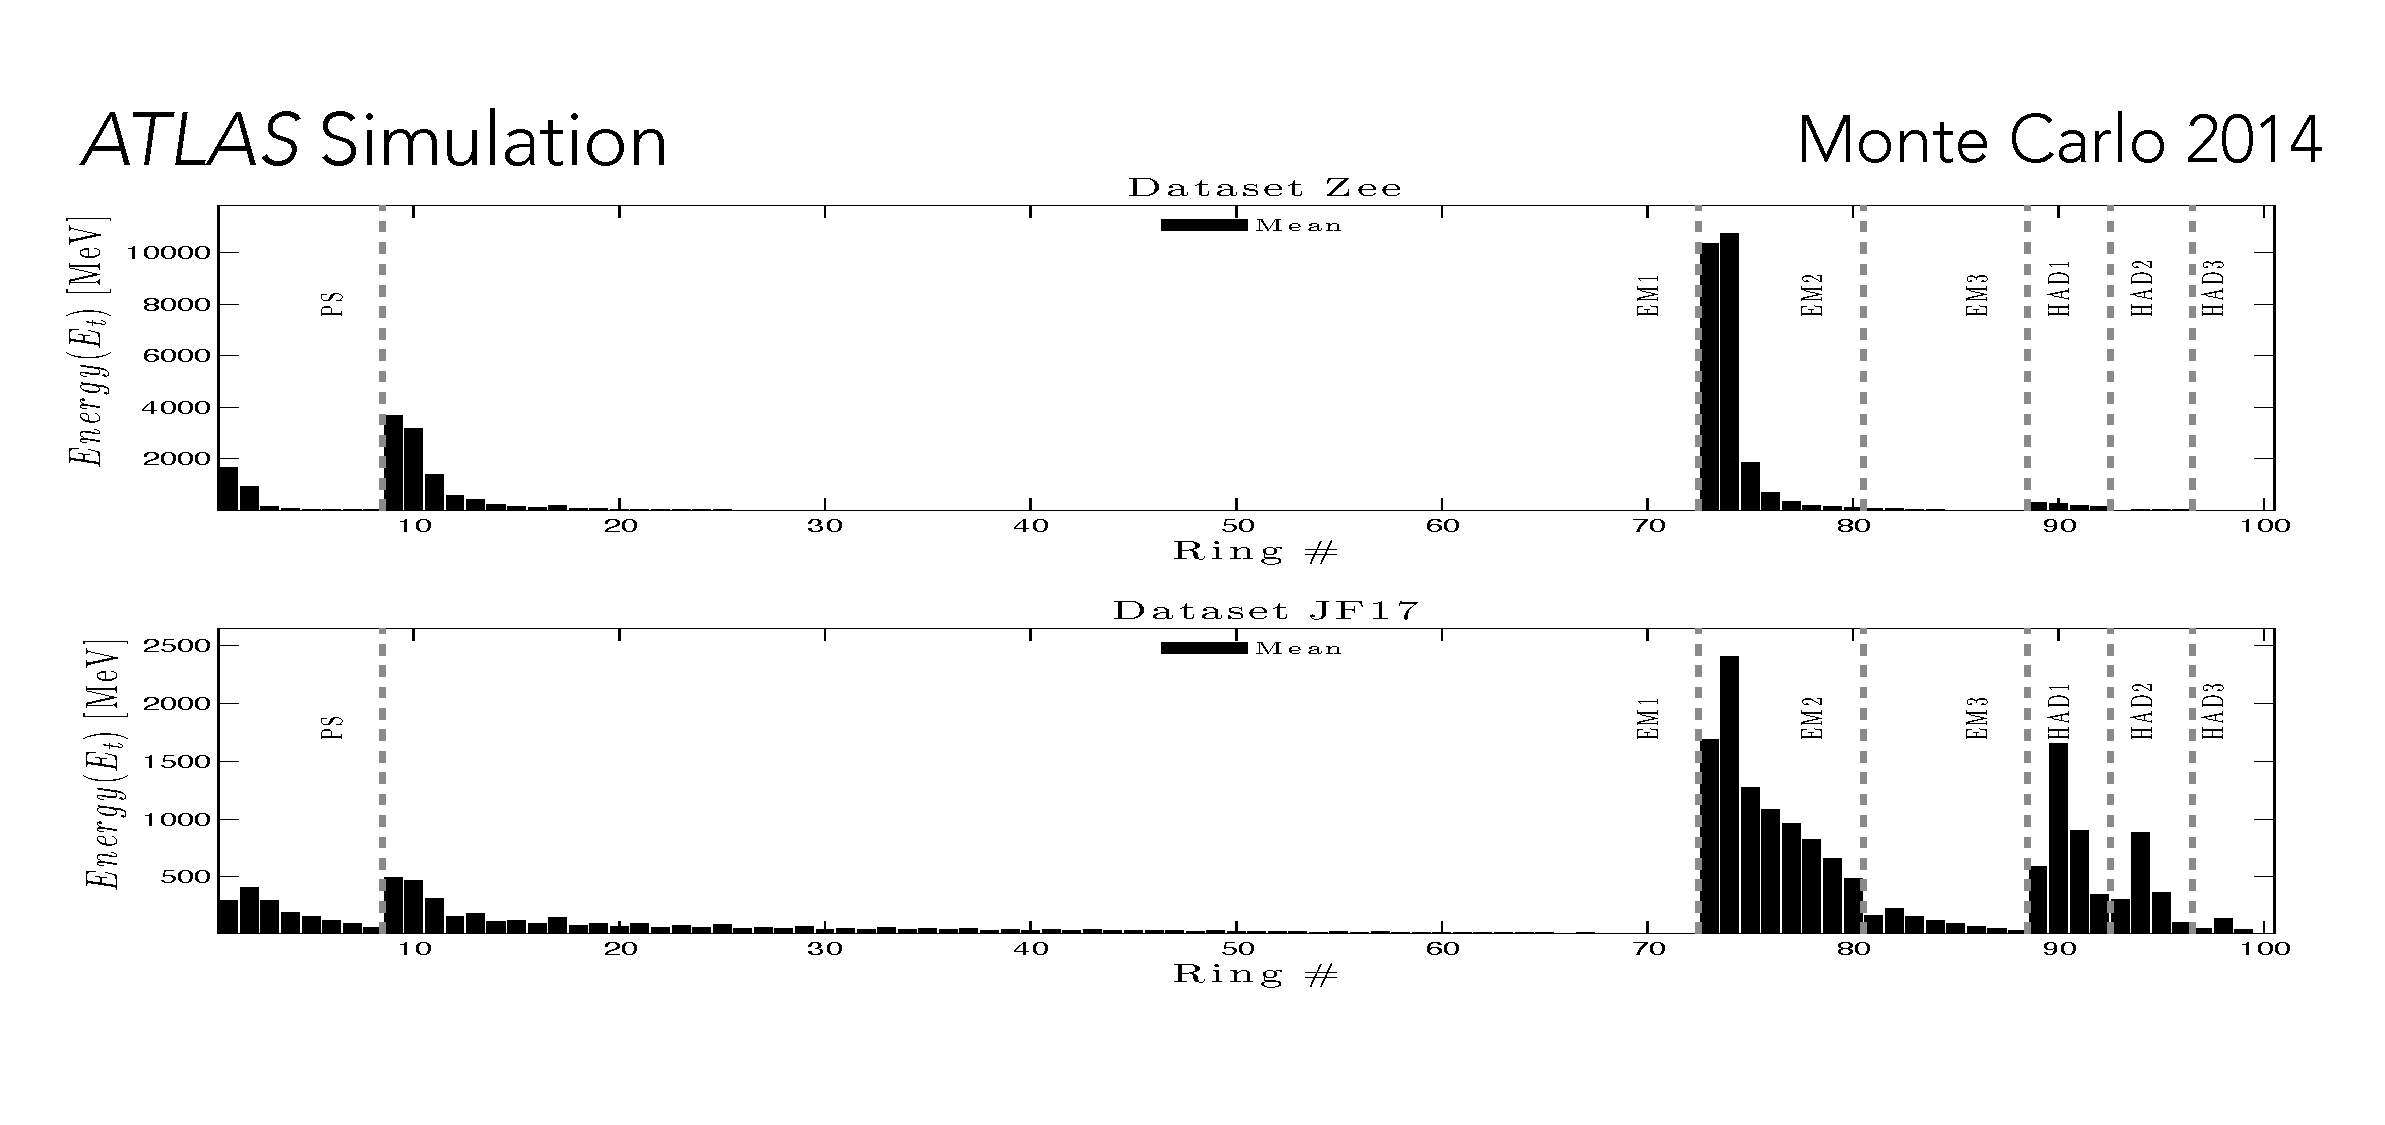
\includegraphics[width=1.0\textwidth]{figures/ringerShape.pdf}
%\caption[Perfil de energia médio para os anéis nas amostras de elétrons e jatos]{Perfis de energia médio, medido em $MeV$, dos anéis para as amostras de elétrons e partículas hadrônicas (jatos).}
%\label{fig:perfil_ringer}
%\end{figure}

\subsection{Estratégia de Trigger}

Os discriminadores neurais são desenvolvidos para a operação no experimento. Assim, a saída da rede neural deve ser comparada com um patamar para a decisão
entre aceitar ou rejeitar a RoI em questão. Esse patamar, porém, pode ser definido por diversas estratégias. Nesse estudo, três estratégias são consideradas.
A primeira considera o ponto de operação do discriminador que consegue a melhor relação entre probabilidade de detecção de elétrons e taxa 
de falso alarme de jatos, segundo o índice SP.

\begin{equation}
SP = \sqrt{ \sqrt{P_{d} \times (1-F_{a})}  \times \frac{(P_{d}+(1-F_{a}))}{2} }
\end{equation}


onde $P_{d}$ é a probabilidade de detecção de elétrons, e $F_{a}$ a taxa de falso alarme do discriminador. A utilização da média geométrica aumenta a sensibilidade em relação as discrepâncias 
entre as duas eficiências. O índice SP pode ser uma alternativa para a escolha de um critério \textit{medium} para o discriminador proposto. As outras duas abordagens consideram a taxa de detecção 
e de falso alarme operadas pelo T2Calo, também, possibilitando a comparação direta entre os dois algoritmos. No entanto, deve-se sempre beneficiar a probabilidade de detecção, já que é esta 
a estratégia comum no sistema \textit{online} de filtragem do ATLAS.


\subsection{Estratégia de Treinamento}


Em todas as abordagens, os conjuntos de RoI de elétrons e jatos foram divididos aleatoriamente em dois conjuntos: o conjunto de treino, utilizado para o ajuste dos 
parâmetros da rede neural com 60\% da base de dados, e o conjunto de teste, utilizado para a avaliação do desempenho de cada discriminador desenvolvido com os 40\% restantes. 
O conjunto de teste também é utilizado como conjunto de validação do treinamento, a fim de evitar o super-treinamento das redes neurais. Normalmente, em experimentos de física de 
partículas, a quantidade produzida de eventos, seja por simulações, seja por aquisições em experimentos reais, é suficiente para a caracterização estatística do processo físico de interesse. 
Dessa forma, não é necessário dividir a base de dados em três conjuntos distintos, como usualmente é feito em projetos de redes neurais.

A arquitetura utilizada foi aquela com melhor desempenho variando-se a quantidade de neurônios na camada escondida da rede neural de 5 até 20.
A rede possui somente uma camada escondida de neurônios e somente um neurônio na camada de saída. Todos os neurônios têm a função tangente hiperbólica 
como função de ativação, onde elétrons são mapeados pelo neurônio de saída em ‘1’ e jatos em ‘-1’.

O algoritmo de treinamento utilizado foi o \textit{resilient backpropagation}  \cite{rprop}, devido à sua rápida convergência.  Os pesos sinápticos da rede são ajustados por batelada, considerando 
o \gls{mse}, como função a ser minimizada. Como a quantidade de RoI de elétrons e de jatos, para alguns casos, é muito diferente, a 
quantidade de RoI utilizadas na batelada é definida pela classe com o menor número de exemplares no treinamento. Posteriormente, para cada época, escolhe-se aleatoriamente 
a mesma quantidade de RoI da classe mais numerosa.

Um método de validação cruzada foi implementado para estimar o impacto da flutuação estatística dos dados utilizados no desempenho dos discriminadores. O método utilizado 
consiste em dividir o conjunto total de dados em $N$ subgrupos, de forma aleatória. Define-se, então, uma quantidade $K$ de sorteios, onde cada sorteio consiste em escolher 
aleatoriamente metade dos $N$ subgrupos para formar o conjunto de treino, e a outra metade para formar o conjunto de teste. A Figura~\ref{fig:crossval} mostra um ilustrativo com a escolha 
de eventos para a validação cruzada.

\begin{figure}[h!t]
\centering
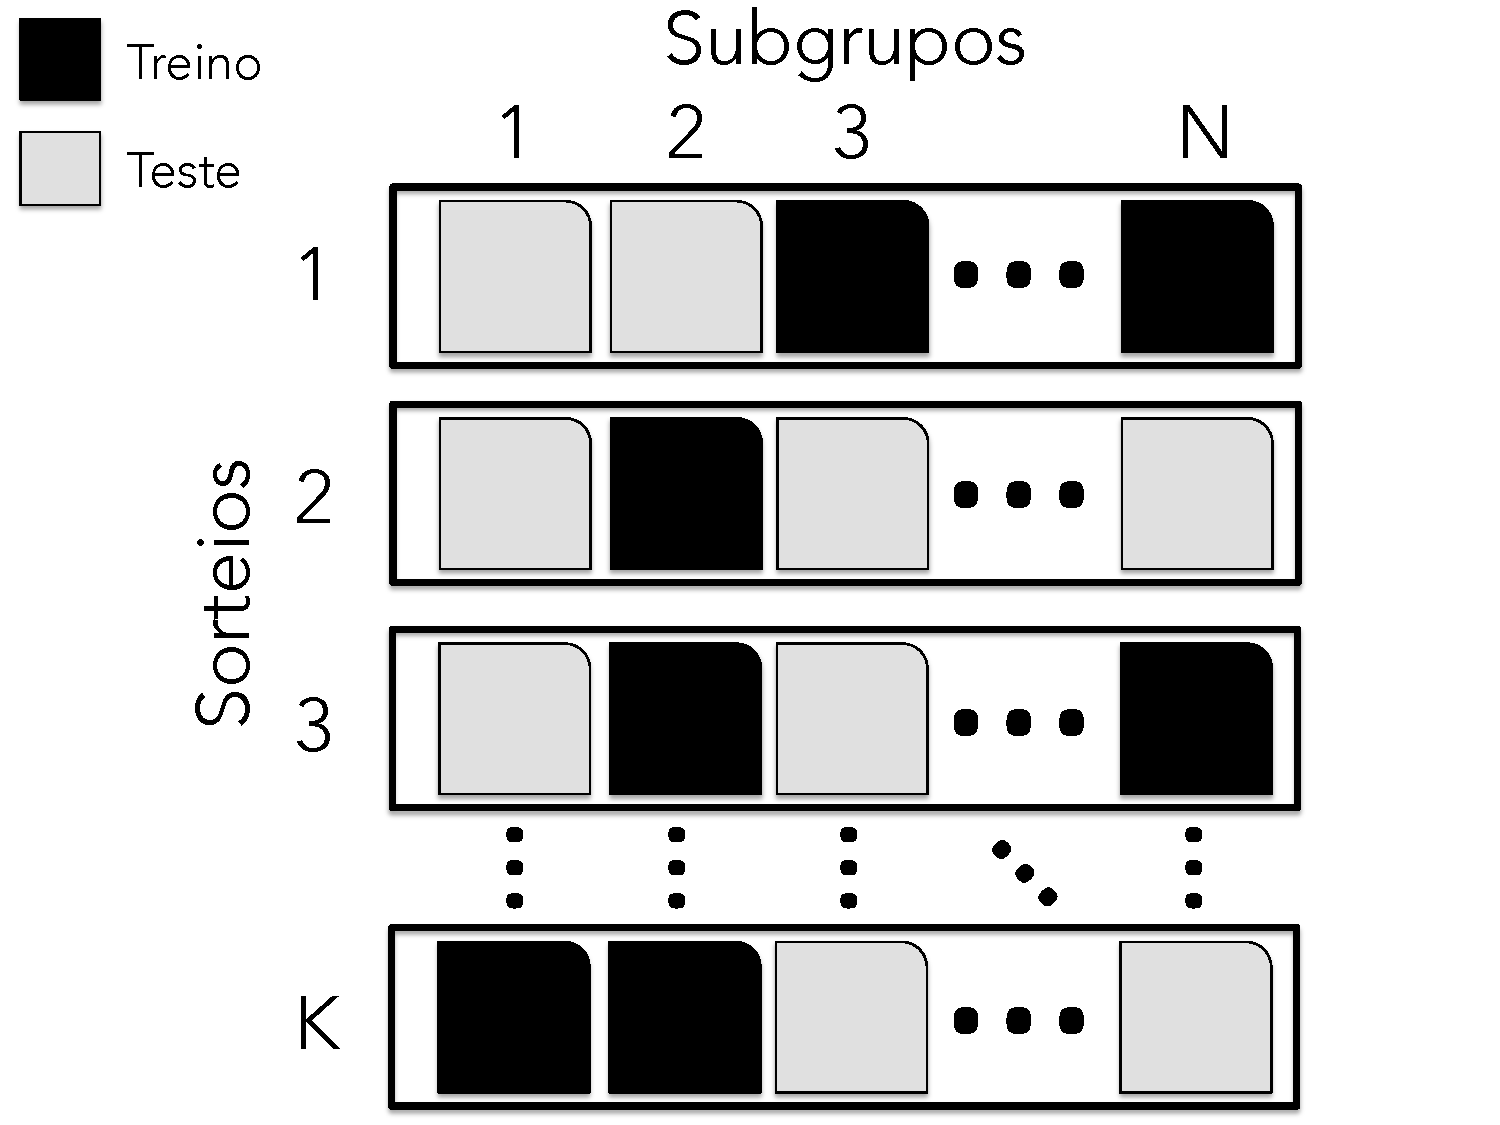
\includegraphics[width=0.4\textwidth]{figures/kfouldFigure.pdf}
\caption[Representação do método de validação cruzada.]{Representação do método de validação cruzada.}
\label{fig:crossval}
\end{figure}

A cada sorteio, escolhe-se aleatoriamente os subgrupos para formar novos conjuntos de treino e teste. Inicializa-se os pesos de 100 discriminadores neurais de forma aleatória, sendo
esta uma técnica de força bruta empregada para escapar de um mínimo local do treinamento. Treina-se os discriminadores para cada sorteio. O discriminador que obtiver o melhor índice SP
avaliado pelo conjunto de teste será arquivado para cada sorteio. Após os $K$ sorteios, 50 sorteios no caso, o desvio padrão dos resultados dos discriminadores arquivados de cada sorteio, em 
conjunto com o valor médio desses resultados, constitui uma boa estimativa do efeito da flutuação estatística dos dados sobre o desempenho da rede neural. No entanto, deve-se escolher 
uma rede dentre as treinadas para diferentes sorteios.

De forma a evitar a polarização do resultado para um determinado  conjunto específico de treino/teste, escolhe-se a rede que obtiver o melhor desempenho utilizando todo o conjunto de dados disponível.
Por fim, antes de alimentar a rede neural, a informação da energia dos anéis deve ser normalizada, de forma a evitar a saturação dos pesos da rede. Diversas normalizações para o 
\textit{Neural Ringer} já foram estudadas~\cite{tese_torres} . Concluiu-se que a normalização mais satisfatória é a divisão do valor de cada anel pela soma do valor de todos os anéis extraídos da RoI.
Embora o \gls{mse} seja escolhido como a função custo, o desempenho da rede é avaliado segundo a sua eficiência na classificação de cada classe. 

A cada época é calculado a probabilidade de detecção e falso alarme, no conjunto de teste, para cada um dos limiares de corte, num intervalo entre [-1,1], testados com a configuração
de pesos atual. Assim, é possível obter o limiar de corte cujo valor de SP foi máximo. De posse desses valores, três critérios de parada sequênciais foram implementados. A parada
por SP prevê a configuração de pesos durante o treinamento cujo SP foi máximo. A parada por detecção salva a configuração de pesos cujo a probabilidade de detecção foi a maior encontrada
durante o treinamento. No caso do falso alarme a ideia é oposta. Ou seja, a melhor configuração será àquela que obtiver o menor falso alarme durante o treinamento.
Caso o índice SP e detecção não aumente e o falso alarme não diminua após um número de épocas, em geral 100, consecutivas, o treinamento é paralisado. Garante-se, também, desta
forma, que não exista  \textit{overfitting} dos resultados. Por fim, três possíveis configurações de pesos referentes a cada um dos critérios discutidos podem ser utilizados posteriormente.



\subsection{\textit{Tag-and-Probe}}

Esse método consiste em utilizar a identificação de duas partículas para a estimação da eficiência de detecção de um determinado algoritmo. É extremamente útil para aplicações em 
dados reais, onde a natureza da partícula observada é desconhecida. A avaliação do desempenho considera um processo físico de interesse, idealmente, aqueles em que o estado 
final de decaimento apresenta duas partículas detectáveis. No caso do bóson de $Z$, por exemplo, o estado final consiste em dois elétrons.

Calcula-se a eficiência a partir da quantidade de objetos \textit{probe} identificados pelo algoritmo avaliado dado que o evento possui um objeto \textit{tag} associado. Ou seja, busca-se 
entre todos os candidatos detectados no evento, aqueles que foram aceitos por um critério extremamente preciso (\textit{tag}), normalmente algum critério \textit{tight}, e possíveis outras considerações. 
Para cada objeto \textit{tag}, busca-se por outros candidatos que, em conjunto com o objeto \textit{tag} selecionado, se aproximem da assinatura do processo físico de interesse (\textit{probe}). 
Normalmente, alguns outros pré-requisitos também são impostos para a seleção desses objetos \textit{probe}. Finalmente, a eficiência é calculada pela razão entre a quantidade de objetos 
\textit{probe} identificados pelo algoritmo avaliado e a quantidade total de objetos \textit{probe} formados.

A imposição de características físicas ao confrontar o par \textit{tag-probe}, de acordo com processo físico de interesse, como, por exemplo, a reconstrução da massa invariante do 
bóson $Z$, aumenta a rejeição do método em relação ao ruído de fundo do experimento. Por isso a sua ampla utilização na colaboração, tanto na avaliação de algoritmos no 
ambiente \textit{online} e \textit{offline}, como na otimização dos cortes utilizados, por exemplo, no algoritmo T2Calo. O método de \textit{tag-and-probe} utilizado nesse estudo utiliza condições e requisitos 
leves para a seleção de cada objeto. Ambos os objetos \textit{tag} e \textit{probe} necessitam de um objeto \textit{offline} associado e que tenha sido aceito pelo critério \textit{tight} de identificação de elétrons. 
Posteriormente, o par formado deve reconstruir a massa invariante do bóson $Z$ no intervalo [80, 100] GeV.  Assim, para o evento ser considerado, um 
dos objetos do \textit{offline} deve ter sido aceito pelo T2Calo (\textit{tag}). A eficiência é calculada, então, como a probabilidade do algoritmo testado aceitar o outro objeto \textit{offline} (\textit{probe}).


\section{Ferramenta de Ajuste dos Pesos da Rede}

Complementar ao problema, o poder computacional para realizar tal experimento utilizando a metodologia de treinamento dos classificadores,
discutida anteriormente, também foi um gargalo que precisou ser otimizado. Assim, optou-se pelo desenvolvimento de um \textit{framework}
que permitisse treinar os inúmeros classificadores de forma totalmente integrada ao ambiente de computação paralela do CERN.
A equação~\ref{eq:total_n_redes} representa o número total de redes neurais que deverão ser treinadas seguindo a metodologia de treinamento, aqui discutida.

\begin{equation}
N_{redes}=N_{sorteios}\times N_{Inits}\times N_{topologias} 
\label{eq:total_n_redes}
\end{equation}

Onde $N_{Sorteios}$ representa o número de sorteios do método de validação cruzada, no caso 50, $N_{Inits}$ o número de inicializações aleatórias
das redes definido como 100 e $N_{Topologias}$ como sendo o número de topologias testadas variando-se o número de neurônios na camada
escondida no intervalo de [5, 20] neurônios, nesse caso 16 topologias avaliadas, totalizando 80 mil redes avaliadas. Dessa forma, o \textit{framework} desenvolvido
precisou conter as seguintes funcionalidades e atender aos seguintes critérios: 

\begin{itemize}

\item Fácil adaptação: O \textit{framework} desenvolvido possui uma interface em \textit{python}, permitindo assim a fácil manutenção e adaptação do código em um
ambiente colaborativo.

\item Ajuste de classificador: o framework possibilita o ajuste de classificadores neurais. O código atual tem como núcleo o \textit{FastNet}, desenvolvido anteriormente pelo 
trabalho~\cite{tese_torres}, em C++. Atualmente o núcleo fornece o treinamento por \gls{rprop} \cite{rprop} e o algoritmo simples de gradiente, ambos
com critérios de parada customizados, no caso da parada pelo índice SP.

\item Adaptação dos dados: O \textit{framework} possibilita a transformação dos dados de saída do \textit{Athena} para o formato \textit{numpy} no \textit{python}. Atualmente isso é feito através da 
entrada de dados formatados, desenvolvido pelo autor deste trabalho em cima do pacote de análise do \textit{trigger} do grupo $e/\gamma$, podendo ser expandido para outros formatos
utilizados pela colaboração

\item Técnica de validação cruzada: Aplicação e medição da técnica de validação cruzada para estimação de flutuações estatísticas.

\item Exportar classificadores: O \textit{framework} deve converter os classificadores a serem utilizados para operação no formato compreendido pelo \textit{Athena}.

%\item Critérios de parada: A aplicação deve conter diferentes critérios de paralisação do treinamento da rede. 

\item Integração com a \textit{grid}: O \textit{framework} deve possibilitar a utilização dos inúmeros computadores pertencentes a \textit{grid} do \gls{cern} para treinar de forma
paralela a grande quantidade de classificadores requeridos.

\end{itemize}

Após a implementação deste \textit{framework} no ambiente do \acrshort{cern}, o tempo de conclusão das análises realizadas para inferir um bom classificador, que 
antes eram de dias, foi reduzido para poucas horas. Permitindo assim, a possibilidade de realizar inúmeros testes e adaptações no método e ou estrutura de
pré-processamento das redes.






|

\chapter{Resultados Obtidos}
\label{cap:resultados}
\glsresetall

Neste Capítulo serão mostrados os resultados referentes ao método discutido neste trabalho. Serão
apresentados a flutuação estatística das rede para cada uma das configurações testadas, a escolha do melhor número
de neurônios da camada escondida, o desempenho dos classificadores durante o treinamento e os resultados de 
eficiência e rejeição do classificador escolhido para operar no sistema de \textit{trigger} de alto nível do ATLAS.

\section{Dados Avaliados}

A seleção do conjunto de sinal formada pela seleção de elétrons extraidos dos dados simulados do decaimento $Z \rightarrow ee$ geraram
um total de 322407 eventos que serão utilizados para treinar o classificador. Para a seleção dos jatos, foram extraídos 11623 eventos
provenientes da simulação de jatos com $E_{T} > 17 GeV$. A seleção dos sinais respeitou as condições discutidas na Seção~\ref{sec:selecao_sinais} 
apresentadas no capítulo anterior. 

A Figura~\ref{fig:perfil_ringer} representa o perfil médio energético, medido em $MeV$, dos anéis para as amostras de elétrons do conjunto de $Z\rightarrow ee$ e de partículas hadrônicas pertencentes 
ao conjunto de jatos em $E_{T}>17 GeV$. Comparando os dois perfis de energia observa-se que as partículas hadrônicas excitam os anéis mais externos de cada camada além de liberar, em média, 
mais energia nas camadas hadrônicas. Assim, os jatos possuem um chuveiro mais largo e profundo que as interações dos elétrons no calorímetro. 

\begin{figure}[h!t]
\centering
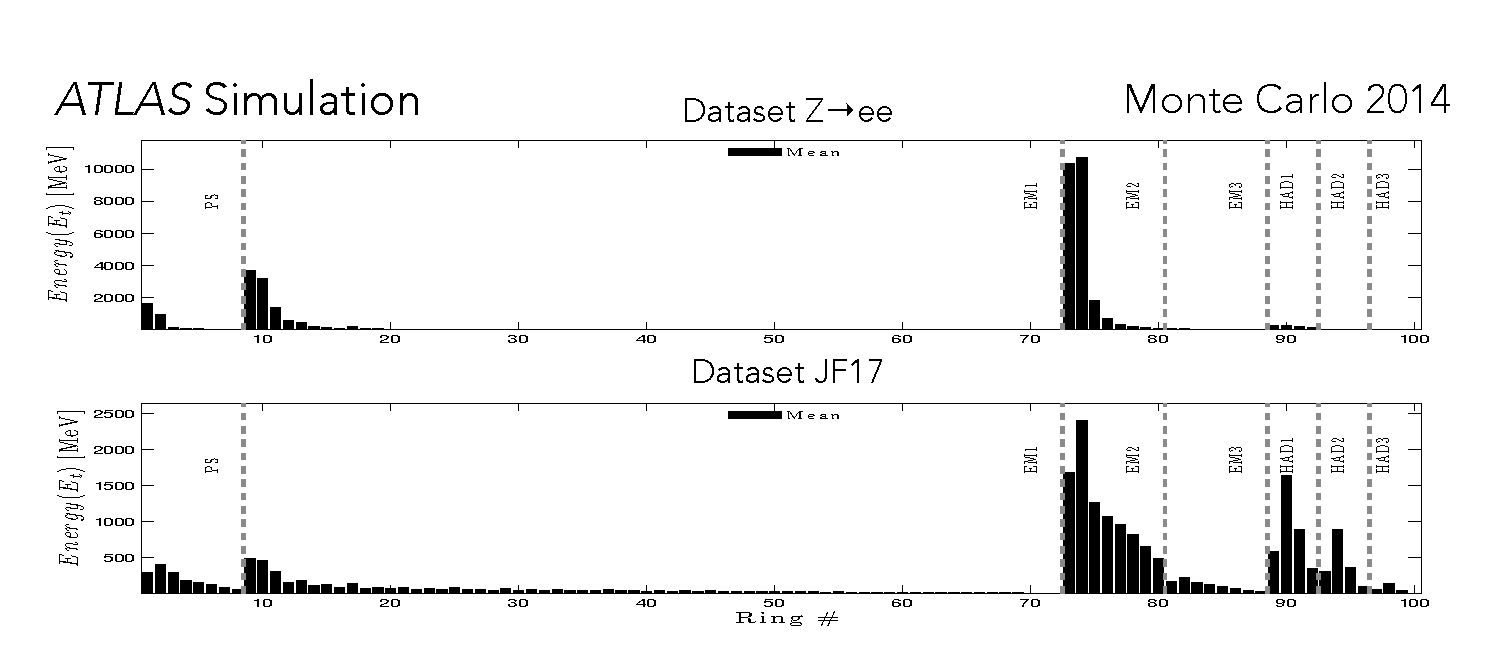
\includegraphics[width=1\textwidth]{figures/plots/ringerShape.pdf}
\caption[Perfil de energia médio para os anéis nas amostras de elétrons e jatos]
{Perfis de energia médio, medido em $MeV$, dos anéis para as amostras de elétrons (superior) e partículas hadrônicas (inferior).}
\label{fig:perfil_ringer}
\end{figure}


\section{Escolha da Rede}

O desempenho das redes de diferentes arquiteturas treinadas a partir dos dados de simulação pode ser observado
na Figura~\ref{fig:escolha_topologia}. O resultado considera a flutuação estatística estimada através do método da validação cruzada para 
os conjuntos de testes. Note que para cada configuração estão representados o valor médio e o desvio padrão dos 
50 sorteios utilizados para cada valor de eficiência (índice SP, probabilidade de detecção e falso alarme).
A escolha da topologia será dada pela observação do comportamento da flutuação do índice SP. Observe que 
o índice aumenta até 8 neurônios e após essa configuração possui um comportamento de crescimento e
decrescimento. Assim, a topologia de 8 neurônios foi selecionada como a melhor configuração a ser estudada.

\begin{figure}[h!t]
\centering
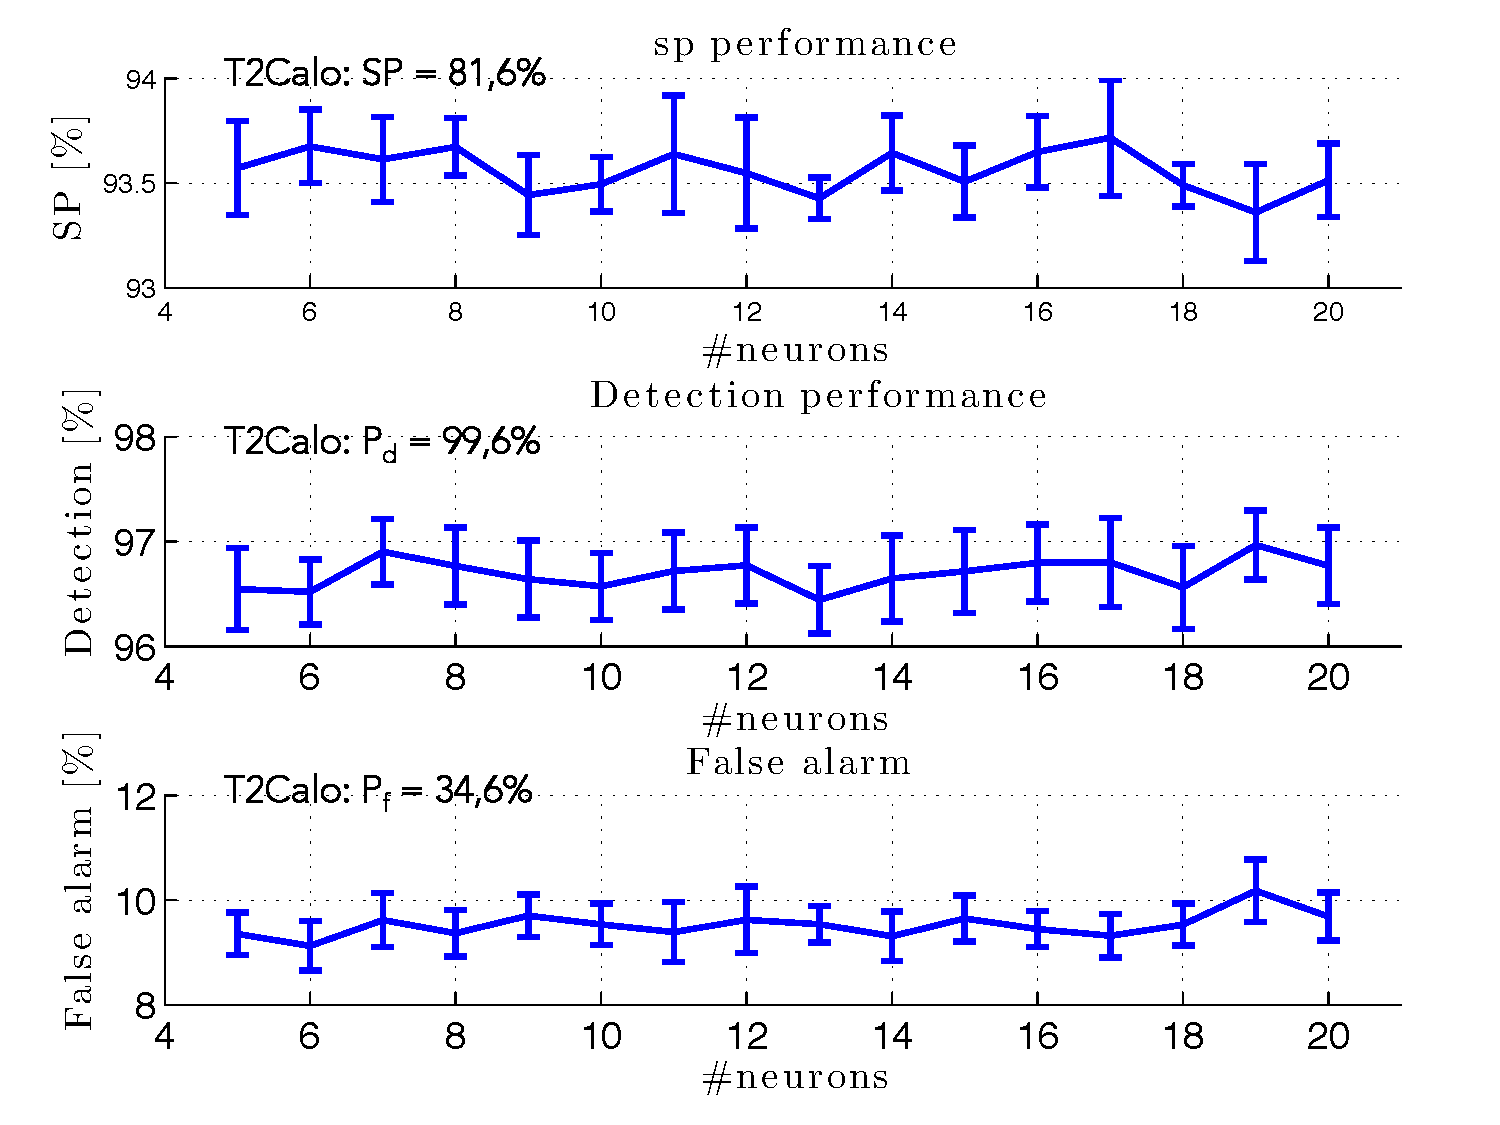
\includegraphics[width=0.7\textwidth]{figures/plots/neurons_evolution.pdf}
\caption[Flutuação estatística segundo o método de validação cruzada para cara arquitetura testada.]
{Flutuação estatística dos conjuntos de testes (50 sorteios) segundo o método da validação cruzada para cada uma das arquiteturas testadas. 
A variação do índice SP, detecção e falso alarme, com suas respectivas incertezas, para cada neurônio na camada escondida no intervalo de [5,20] neurônios,
estão representadas de cima para baixo respectivamente.}
\label{fig:escolha_topologia}
\end{figure}


Na Tabela~\ref{tab:flutuacao_validacao_cruzada}, estão representados os valores e suas respectivas incertezas
para as redes de 8 neurônios. Na última linha da tabela, estão representados os valores de eficiência do algoritmo
de referência utilizado para ajustar as redes de acordo com seu respectivo critério de parada durante o treinamento.
Na primeira linha, estão representados os valores para as redes ajustadas para valores próximos à taxa de detecção (Verde) do
algoritmo de referência. Por sua vez, a terceira linha representa os valores para as redes ajustadas para o mesmo
falso alarme (Azul) do algoritmo de referência.

\begin{table}[]
\centering
\begin{tabular}{cccc}
\hline
 & DET {[}\%{]} & SP {[}\%{]} & FA {[}\%{]} \\ \hline
ringer (pd) & \cellcolor[HTML]{9AFF99}99.6343$\pm$0.0034 & 90.4081$\pm$0.2422 & 18.3691$\pm$0.4603 \\
ringer (sp) & 96.6829$\pm$0.3708 & 93.5197$\pm$0.2046 & 9.5902$\pm$0.4719 \\
ringer (fa) & 99.9665$\pm$0.0048 & 81.7590$\pm$0.0315 & \cellcolor[HTML]{BBDAFF}34.6105$\pm$0.0566 \\ \hline
T2Calo & \cellcolor[HTML]{9AFF99}99.6349 & 81.6081 & \cellcolor[HTML]{BBDAFF}34.6124 \\ \hline
\end{tabular}
\caption[Valores de eficiência de detecção (DET), índice SP e taxa de falso alarme (FA) para a topologia escolhida.]
{Valores de eficiência de detecção (DET), índice SP e taxa de falso alarme (FA) para a topologia de 8 neurônios escolhida. 
As incertezas de cada valor foram calculadas utilizando o método de validação cruzada. Na última linha da tabela são apresentados os valores de referência 
do algoritmo T2Calo obtidos para ajustar as redes neurais nos casos de detecção e falso alarme. As redes ajustadas pelo máximo SP não possuem uma 
referência, uma vez que elas buscam o máximo índice obtido dentro de cada treinamento realizado.}
\label{tab:flutuacao_validacao_cruzada}
\end{table}

A seleção das melhores redes dentro de cada caso comparativo é obtida pelo cálculo dos valores de eficiência dos classificadores utilizando
todo o conjunto de dados disponível. Essa técnica é bastante utilizada pois durante a validação cruzada podem ocorrer casos em que um conjunto
de teste é mais fácil que outros. Assim, para evitar a polarização dos resultados, todo o conjunto de dados é utilizado para o cálculo das 
eficiências de cada uma das 50 redes treinadas referentes a topologia escolhida.


\subsection{Avaliação do Treinamento das Redes Selecionadas}

A avaliação do treinamento das melhores redes selecionadas para cada um dos critérios de ajuste estão representados nesta sub-seção.
Para os critérios de melhor índice SP e melhor taxa de detecção percebeu-se que as configurações de pesos foram obtidas do 
mesmo treinamento. Embora um treinamento retorne três possíveis configurações de pesos ajustadas, apenas as duas configurações
citadas serão utilizadas. Sendo, também, as melhores configurações obtidas dentro dos 50 treinamentos realizados para essa configuração
e critérios.

Na Figura~\ref{fig:ratevalues_sp_det}, estão representadas as curvas de evolução do treinamento para cada um dos critérios avaliados.
Para melhorar a representação gráfica, o falso alarme foi representado como a capacidade de identificação de eventos da classe de jatos. 
Assim, quanto mais próximo de '1' melhor será a rejeição do classificador aos jatos.
As épocas onde ocorreram as melhores configurações de pesos para cada um dos casos estão marcadas em cada uma das curvas.
Vale ressaltar que o treinamento só é paralisado após um determinado número de épocas ser atingido depois do último critério de parada ter sido
habilitado. Assim, em um único treinamento são extraídos três configurações de pesos referentes a cada um dos casos.
Na Figura~\ref{fig:mse_sp_det}, está representada a evolução do \acrshort{mse} para os conjuntos de treino e teste.

\begin{figure}[ht!]
    \begin{center}
        \subfigure[A evolução das curvas de detecção (Preto),  Falso Alarme (Azul) e o índice SP (Magenta) para o treinamento selecionado.]
         {
            \label{fig:ratevalues_sp_det}
            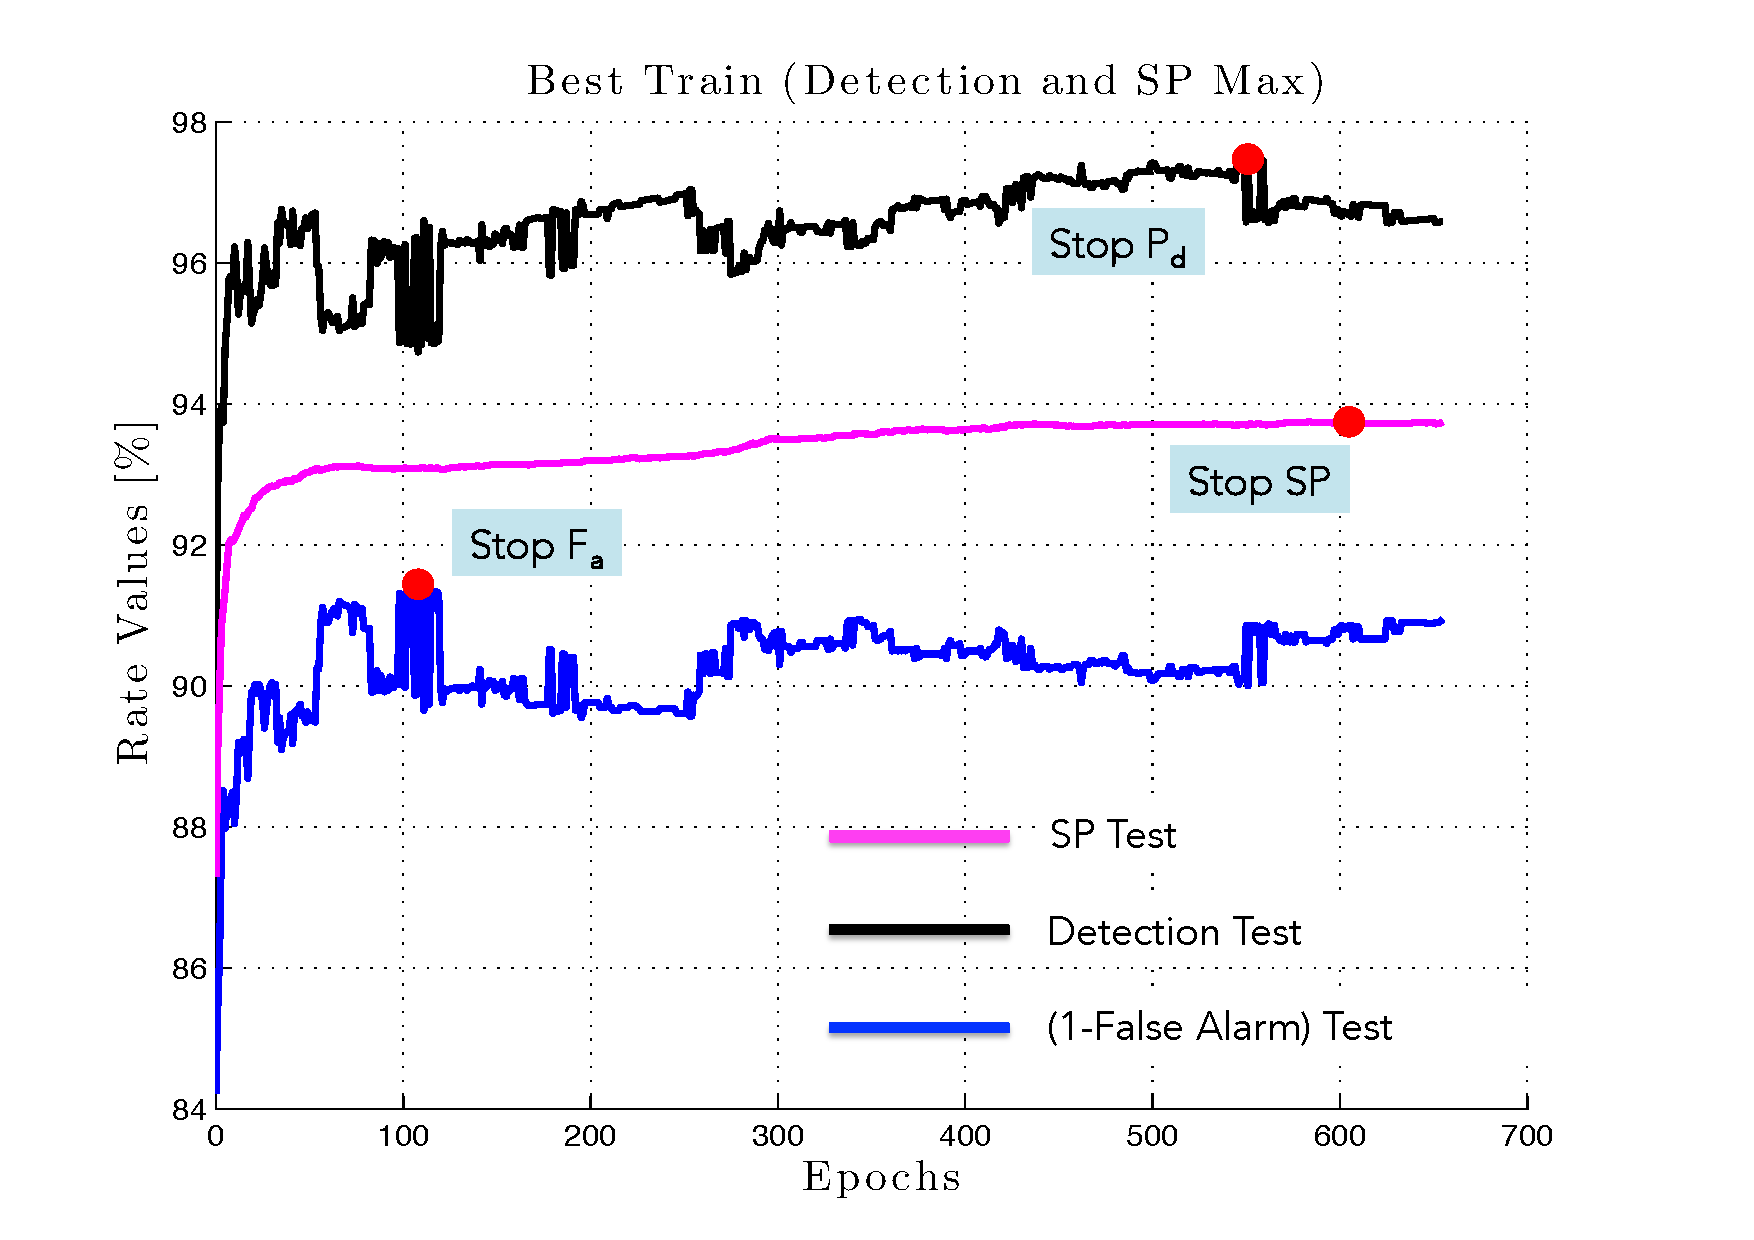
\includegraphics[width=0.46\textwidth]{figures/plots/ratevalues_evolution_sp_det.pdf}
        }\hspace{0.02\textwidth}
        \subfigure[As curvas de evolução do \gls{mse} para os conjuntos de treino e teste.]
        {
            \label{fig:mse_sp_det}
            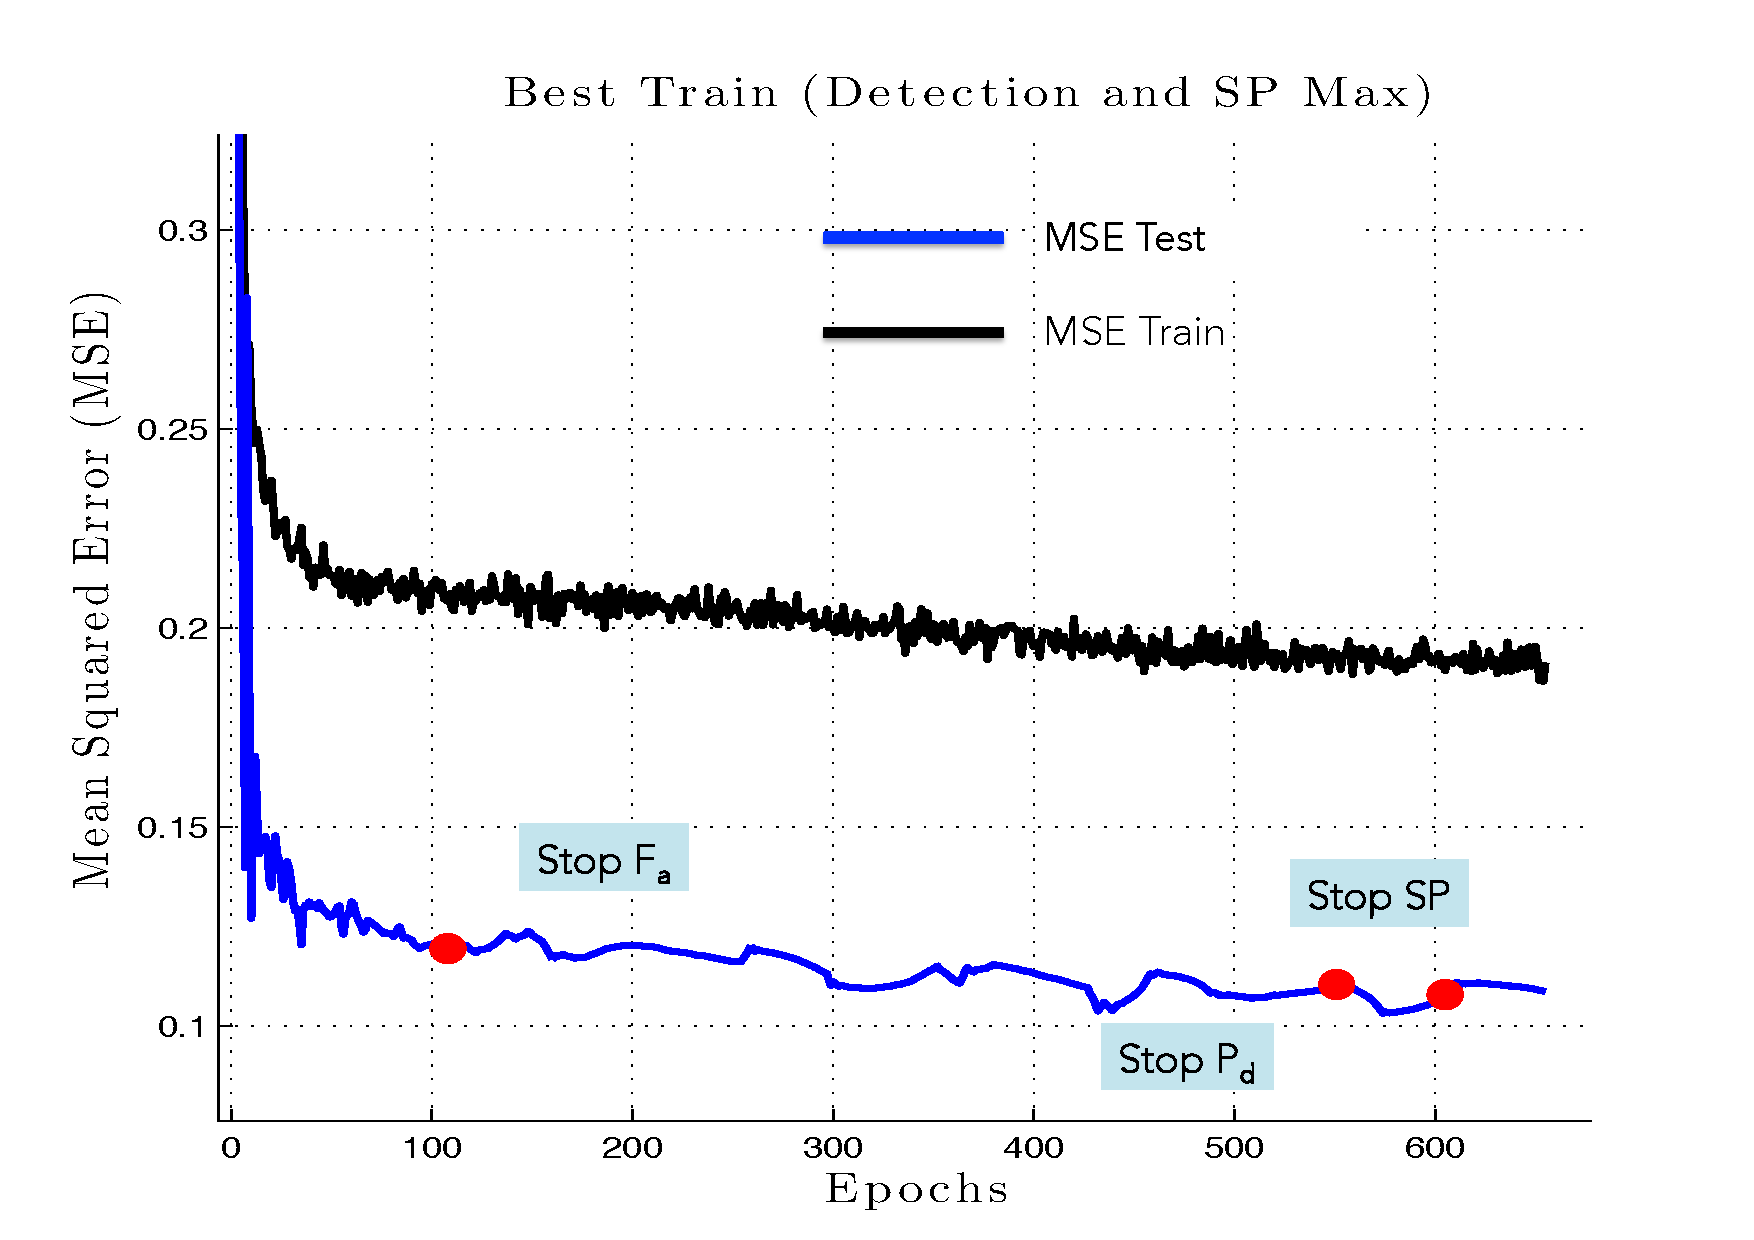
\includegraphics[width=0.46\textwidth]{figures/plots/mse_evolution_sp_det.pdf}
        }\\ 
    \end{center}
    \caption[As curvas de treinamento para as redes selecionadas pelos critérios de melhor SP e detecção.]{
    As curvas de treinamento para as redes selecionadas pelos critérios de melhor SP e detecção.}
\end{figure}

Entretanto, as Figuras~\ref{fig:ratevalues_fa} e~\ref{fig:mse_fa} representam a evolução das curvas de eficiência e \gls{mse}
ao longo do número de épocas para o treinamento selecionado com ajustes pelo falso alarme. É possível notar que nesse
treinamento, o número máximo de épocas atingidos foi menor que no caso anterior.


\begin{figure}[ht!]

    \begin{center}
    
        \subfigure[A evolução das curvas de detecção (Preto),  Falso Alarme (Azul) e o índice SP (Magenta) para o treinamento selecionado.]
         {
            \label{fig:ratevalues_fa}
            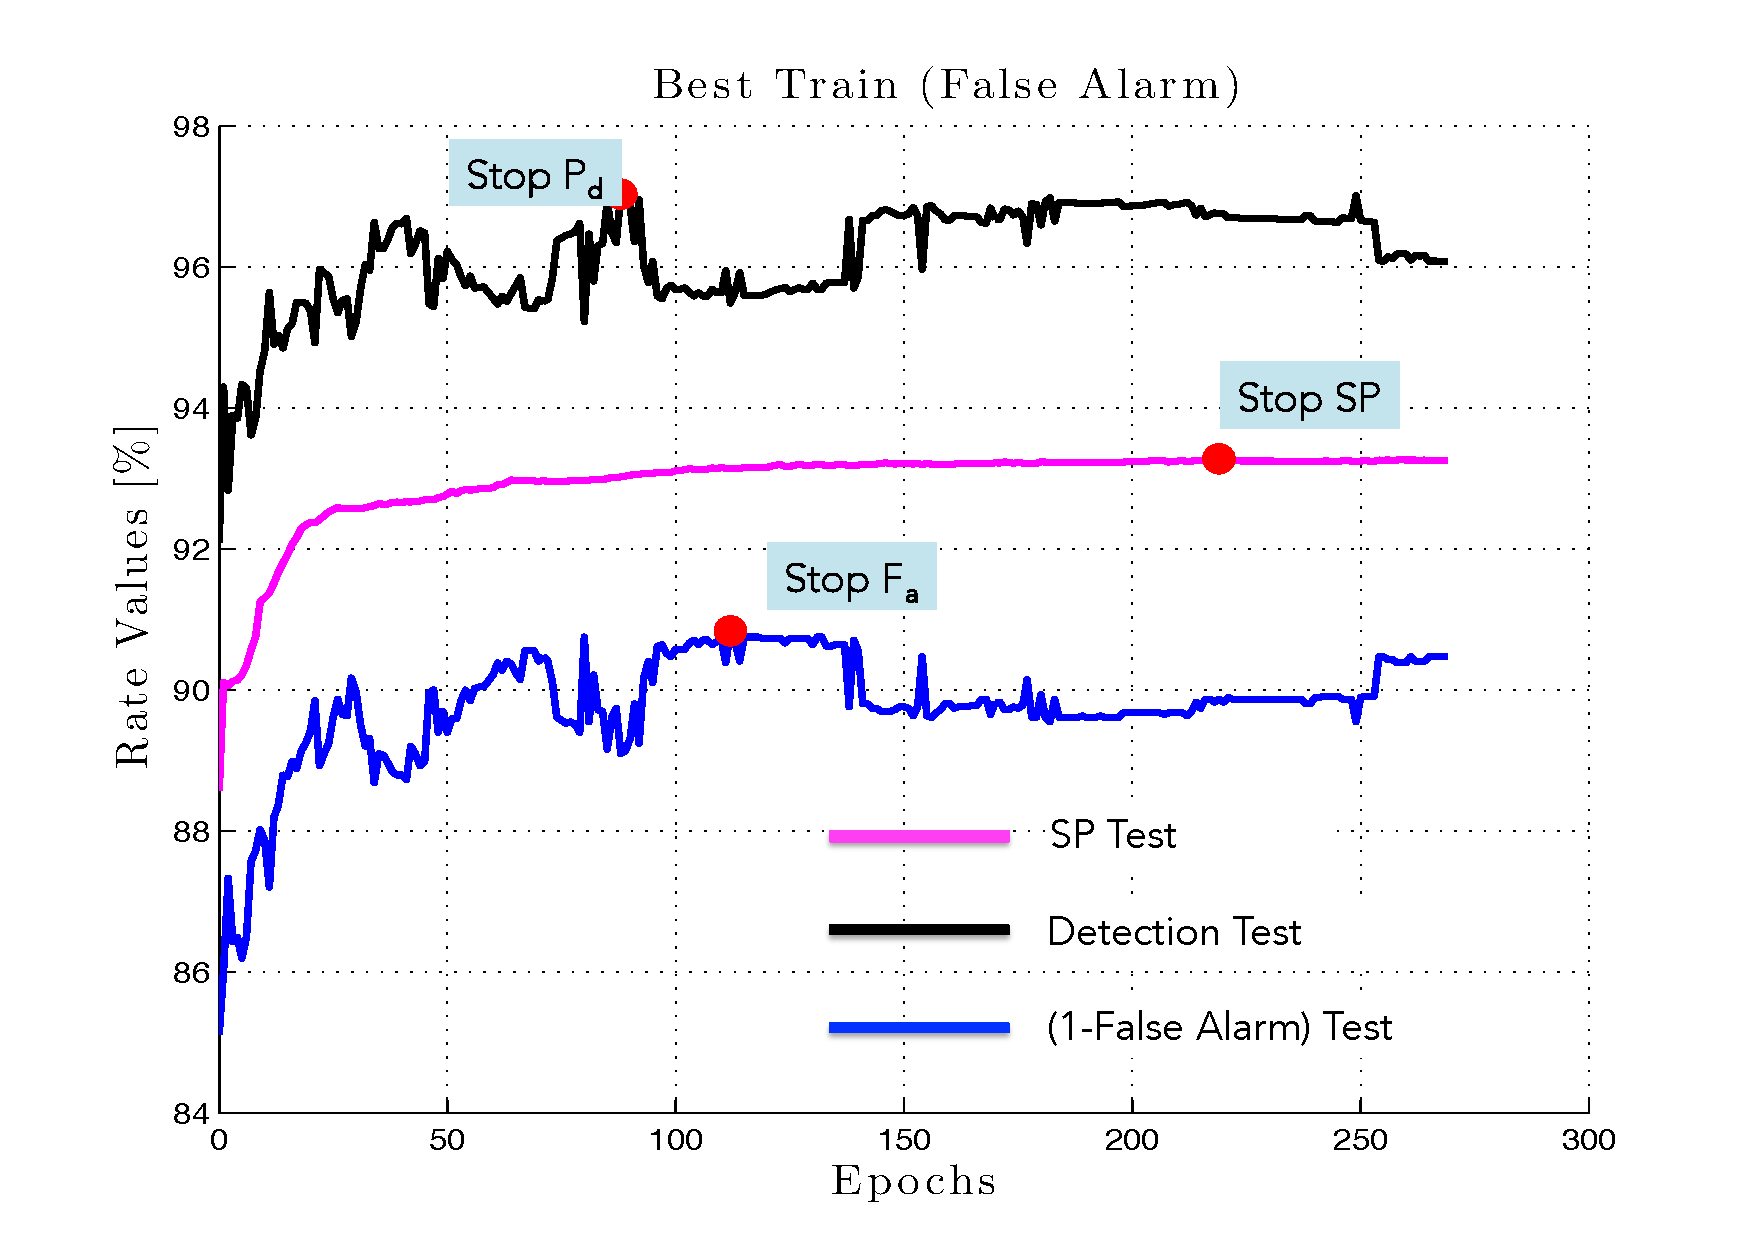
\includegraphics[width=0.46\textwidth]{figures/plots/ratevalues_evolution_fa.pdf}
        }\hspace{0.02\textwidth}
        \subfigure[As curvas de treinamento para as redes selecionadas pelos critérios de melhor SP e detecção.]
        {
            \label{fig:mse_fa}
            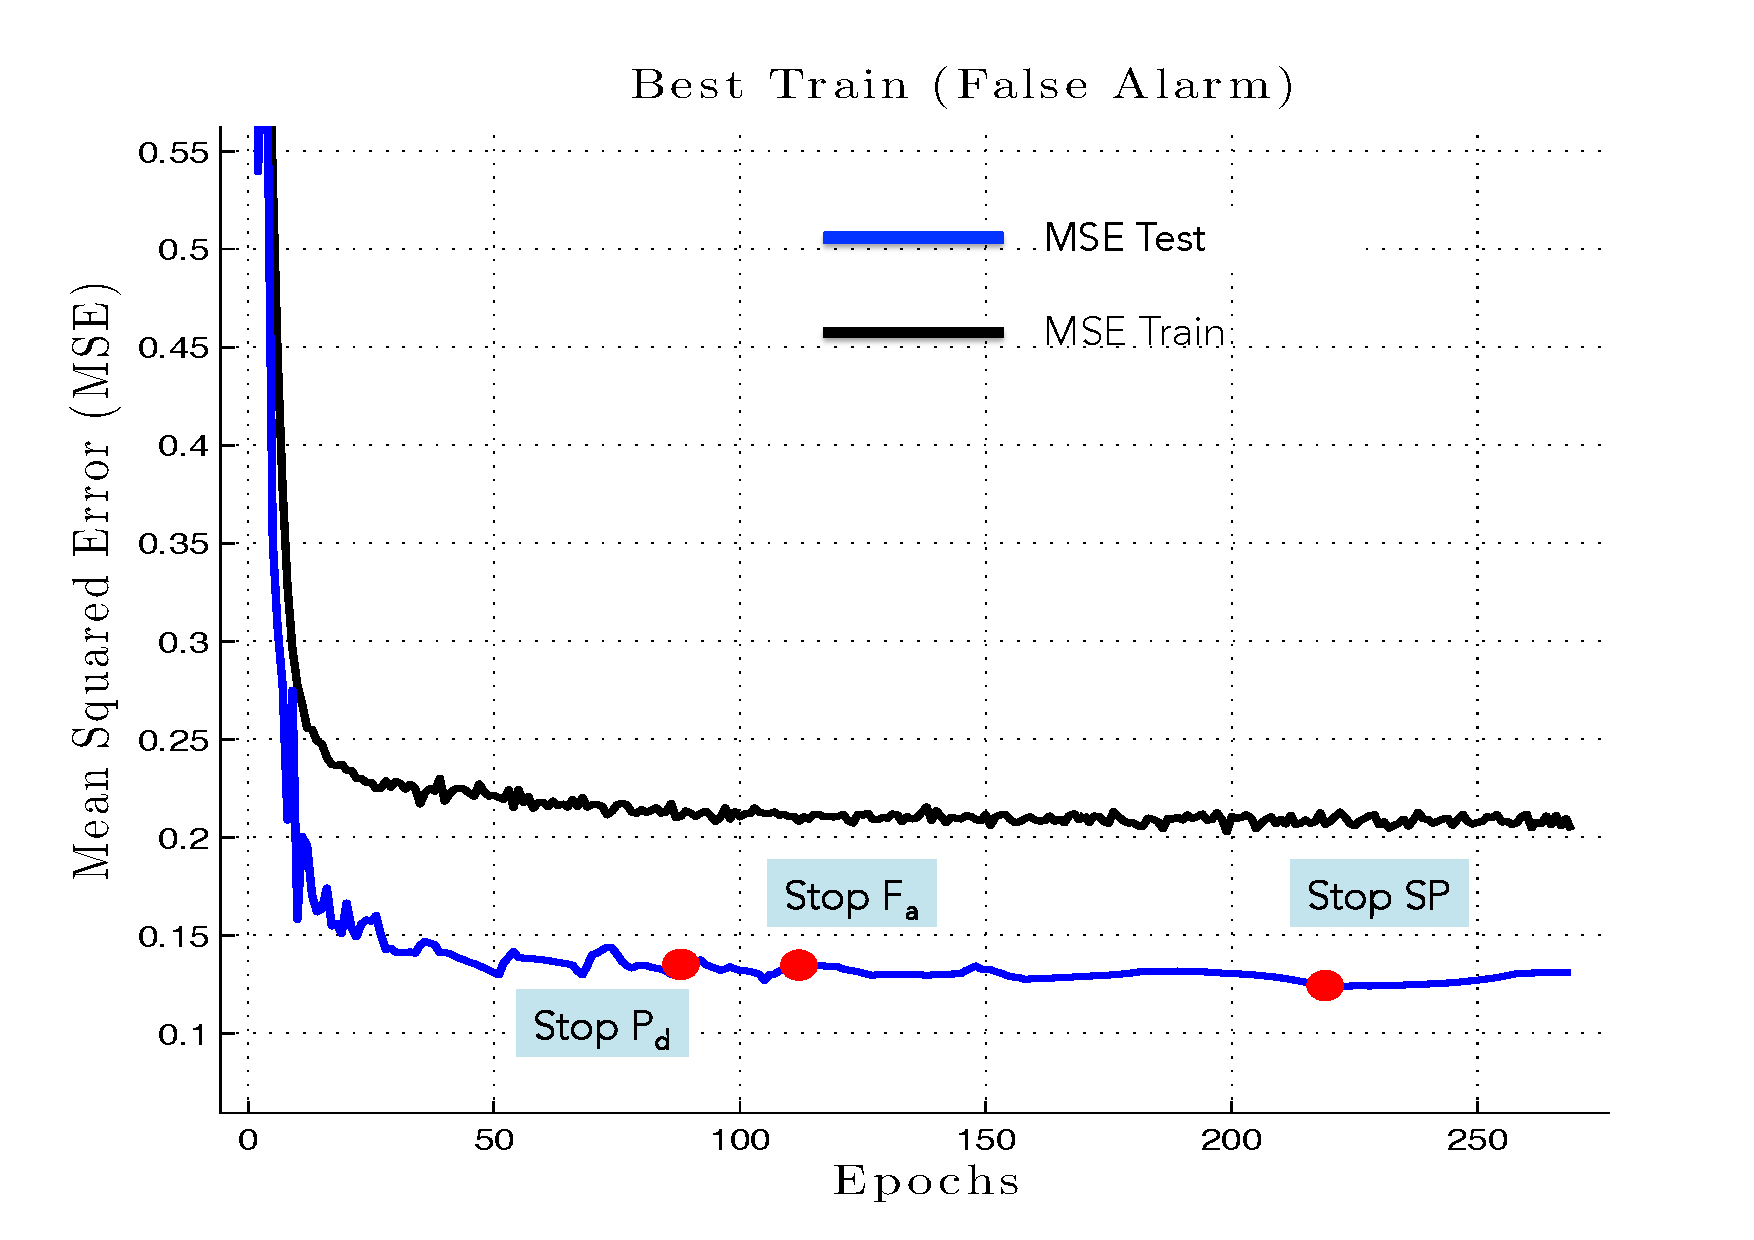
\includegraphics[width=0.46\textwidth]{figures/plots/mse_evolution_fa.pdf}
        }\\ 

    \end{center}
    \caption[As curvas de treinamento para a rede selecionada pelo critério de melhor falso alarme.]{
    As curvas de treinamento para a rede selecionada pelo critério de melhor falso alarme.}

\end{figure}



%\newpage
A Figura~\ref{fig:roc} apresenta a curva \gls{roc} para os classificadores selecionados para cada um dos critérios de ajustes
utilizados. O ponto de operação do algoritmo de referência de cada um dos ajustes também é mostrado. Graficamente,
percebe-se que para uma mesma taxa de detecção do algoritmo de referência de $99,6\%$, o classificador selecionado
para operar nessa faixa possui um falso alarme de $18,3\%$. Representando, assim, uma redução por um fator de $\sim2$ 
na taxa de falso alarme


Assim, levando em consideração que o problema está sendo aplicado em um ambiente de filtragem \textit{online} e que a 
probabilidade de detecção dos eventos é extremamente crítica nessas aplicações, foi selecionado a rede cuja taxa de
detecção foi ajustada pela do algoritmo de referência. Essa estratégia, embora mantenha a taxa de detecção, irá reduzir a
quantidade de eventos que não são interessantes para a física em \textit{triggers} superiores. Reduzindo, assim, por exemplo, o 
número de vezes que os algoritmos mais complexos, como o \textit{tracker}, serão aplicados na cadeia de \textit{trigger}.

\begin{figure}[h!t]
\centering
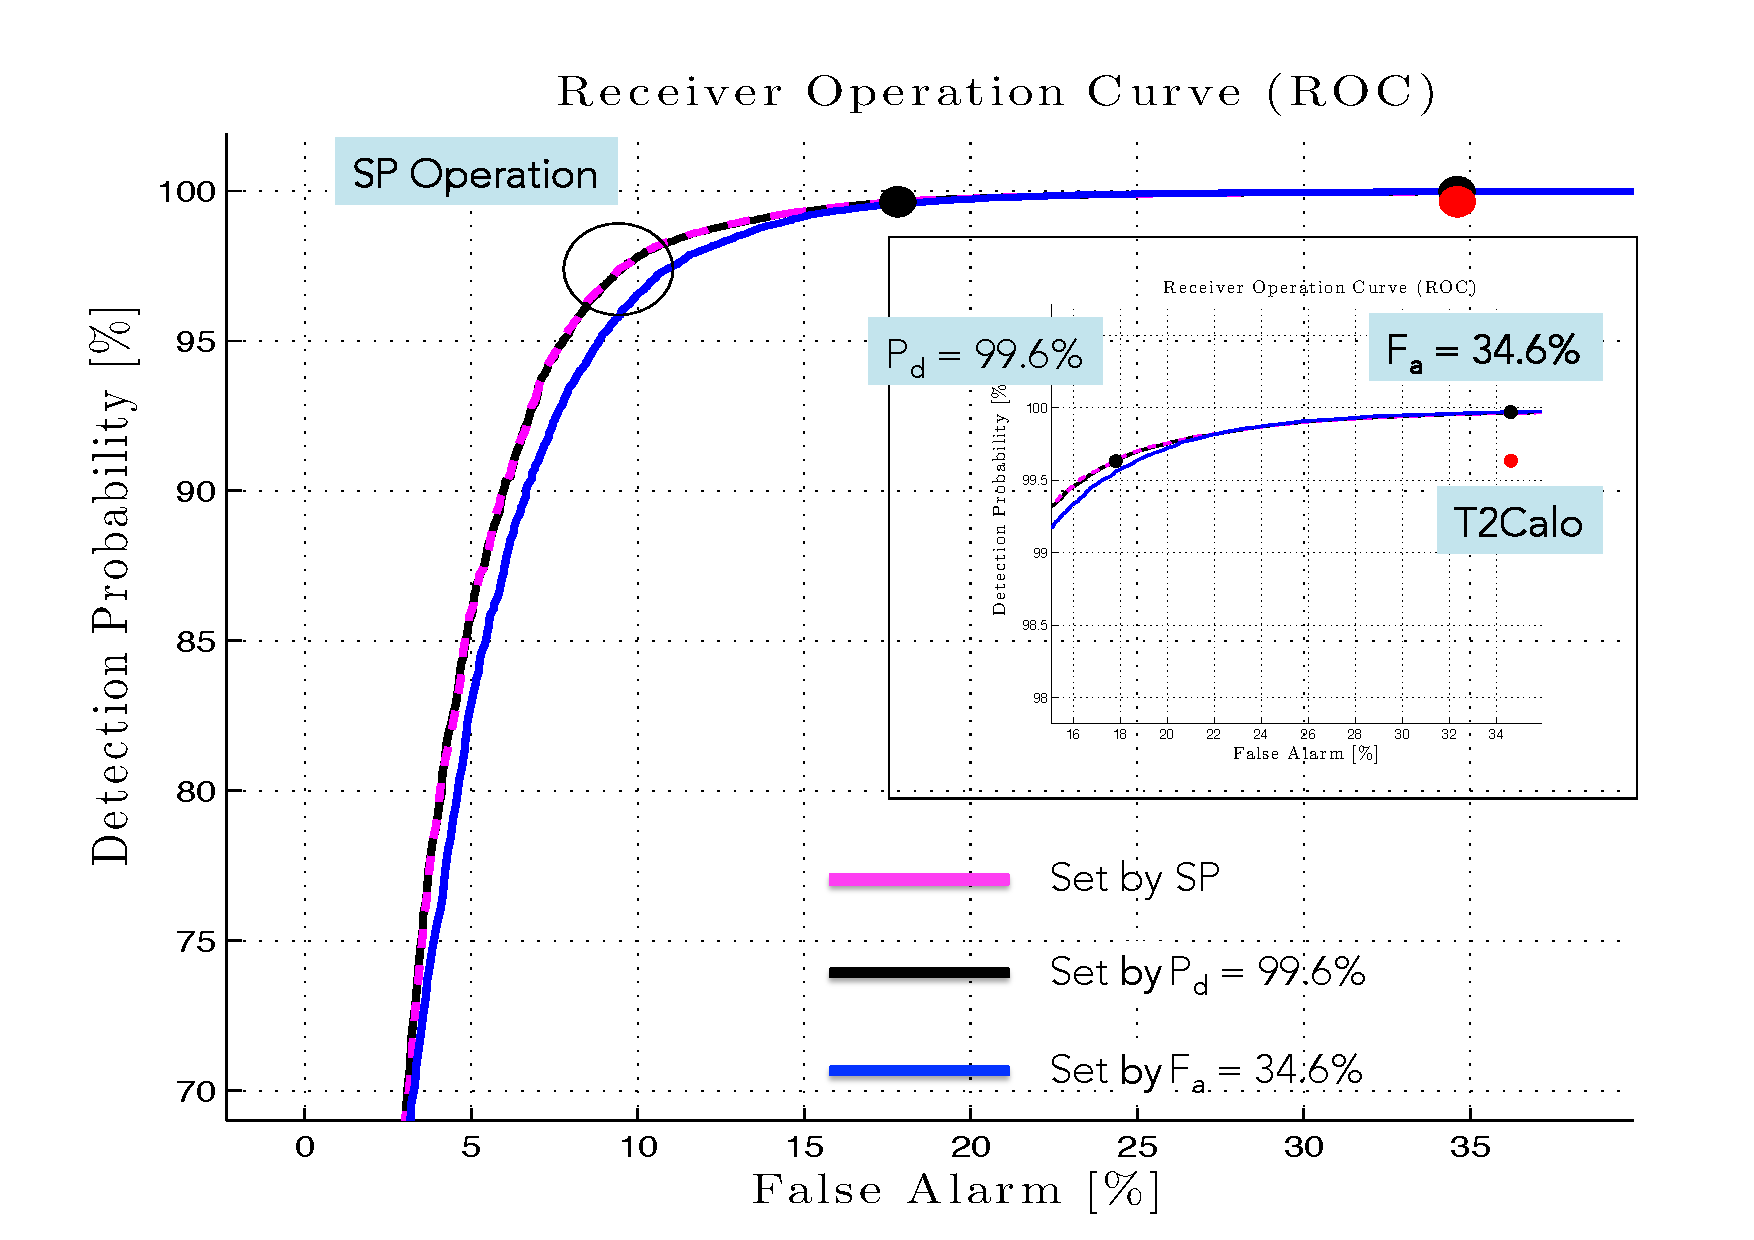
\includegraphics[width=0.7\textwidth]{figures/plots/roc.pdf}
\caption[Curva \gls{roc}]{Curva \gls{roc} e os pontos de operações ajustados para cada um dos discriminadores selecionados.}
\label{fig:roc}
\end{figure}



\section{Eficiências pelo Método de \textit{Tag-and-Probe}}

O classificador ajustado para operar com aproximadamente a mesma probabilidade de detecção do algoritmo de referência foi 
utilizado para emular a resposta do \textit{trigger} dentro do ambiente de simulação da colaboração.  
Nesta seção, serão apresentados os resultados de eficiência dos algoritmos avaliados com amostras de eventos gerados
pelo algoritmo de \textit{tag-and-probe} oficial do grupo $e/\gamma$.

Os pares gerados pelo algoritmo de \textit{tag-and-probe} foram gerados pelo conjunto de amostras do decaimento do $Z\rightarrow ee$
obtidos por simulação de Monte Carlo. Assim, as eficiências do \textit{trigger} na etapa de calorimetria rápida foram calculadas
para a \textit{chain} de referência e a nova proposta. A eficiência do método é dada pelo número
de \textit{probes} aceitos pelo algoritmo de hipótese testado dividido pelo número total de pares formados pelo método. A Figura~\ref{fig:tap_et}
apresenta as eficiência do \textit{trigger} em função da variação de energia para as respectivas \textit{chains}.

\begin{figure}[h!t]
\centering
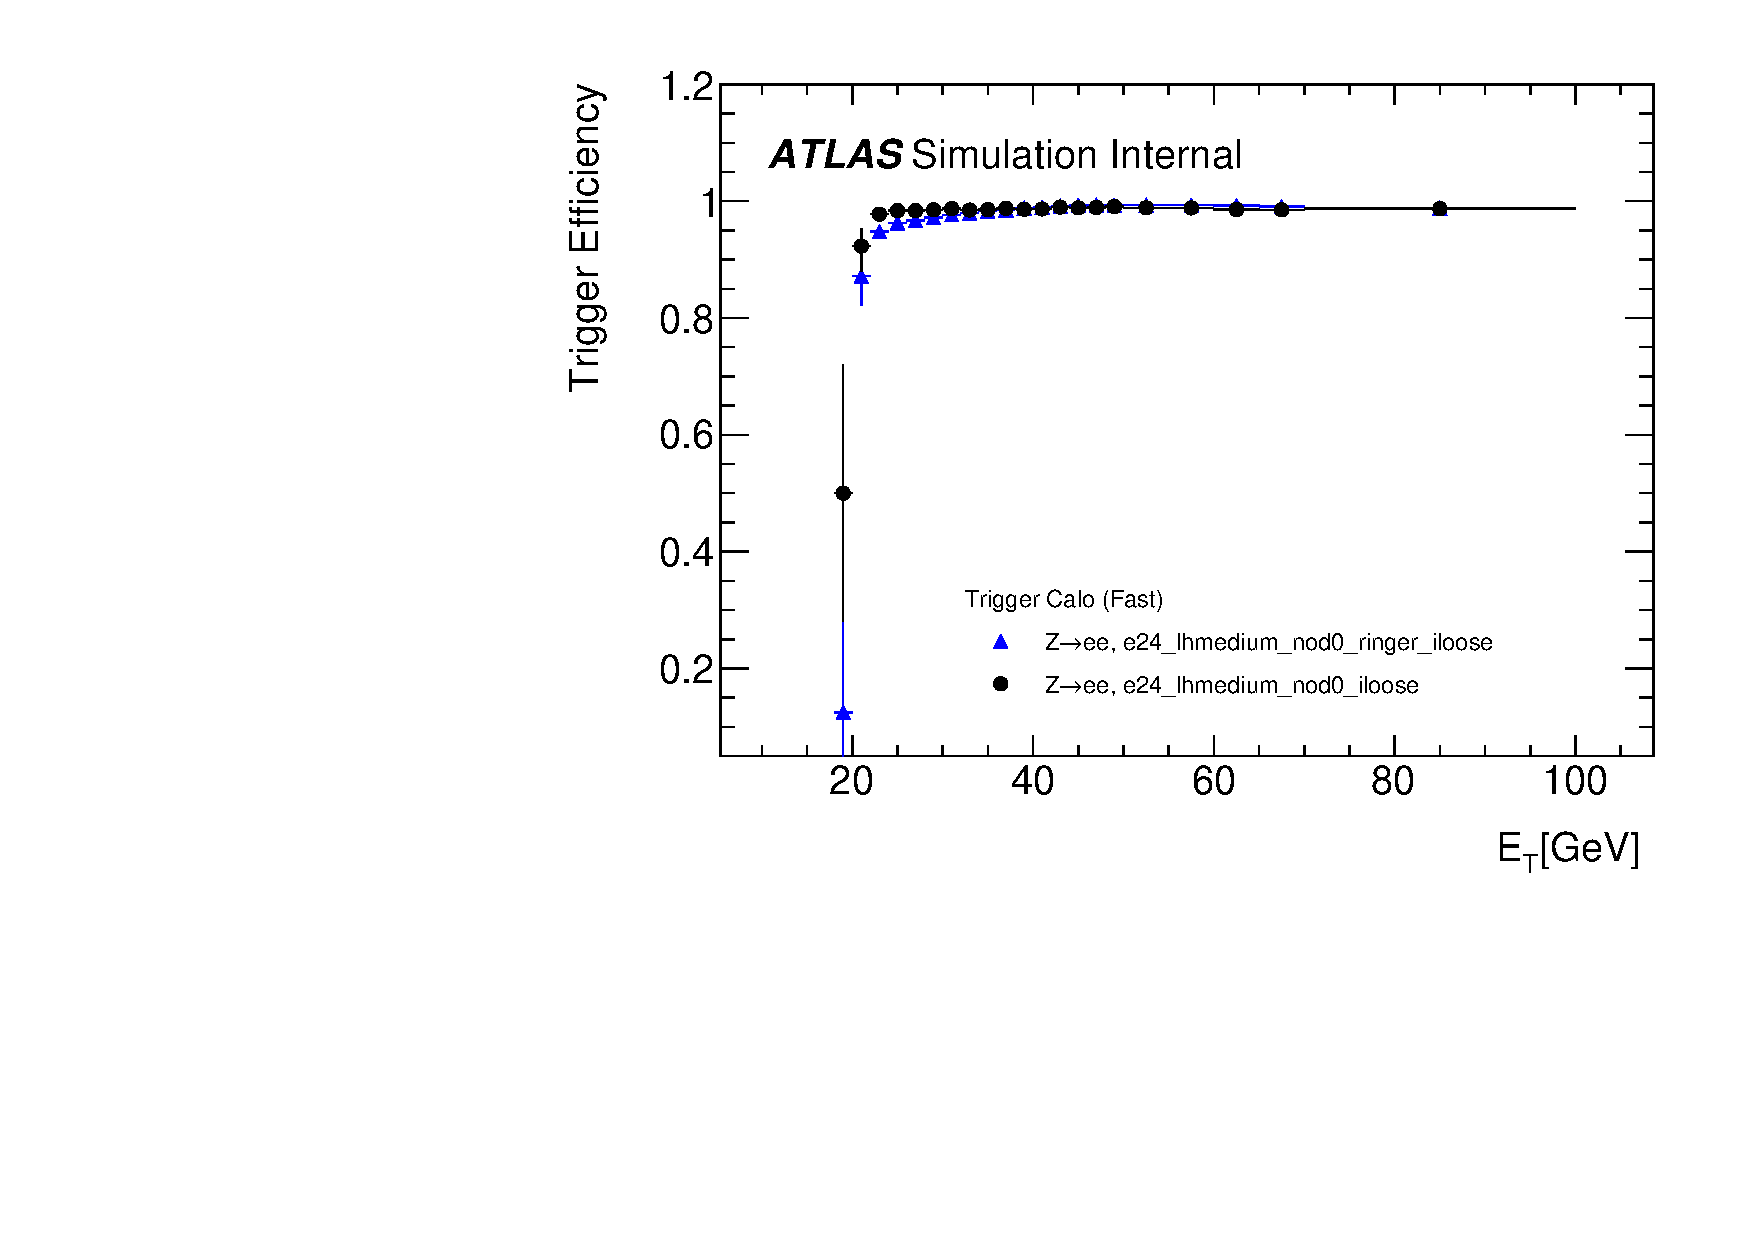
\includegraphics[width=0.6\textwidth]{figures/plots/plot_e24_lhmedium_hlt_eff_et_tap.pdf}
\caption[As eficiências do método de \textit{tag-and-probe} em função da energia em $GeV$.]{
As eficiências do método de \textit{tag-and-probe} em função da energia em $GeV$ para cada uma das \textit{chains} listadas.}
\label{fig:tap_et}
\end{figure}


Para as duas curvas de eficiência em função da energia, note que a subida da \textit{chain} do \textit{ringer} é mais lenta que o algoritmo de referência.
Esse efeito é atribuido ao ajuste dos cortes de aceitação nessa região. No caso, o algoritmo de referência possui diferentes cortes em função
da faixa de energia do evento. Diferentemente do proposto, que ajusta o limiar de corte do classificador olhando para toda
a faixa de energia.  A Figura~\ref{fig:tap_eta} mostra a eficiência de detecção dos \textit{probes} em função da região em $\eta$ no detector.  
Novamente, o algoritmo de referência também possui diferentes cortes para cada região do detector. 

\begin{figure}[h!t]
\centering
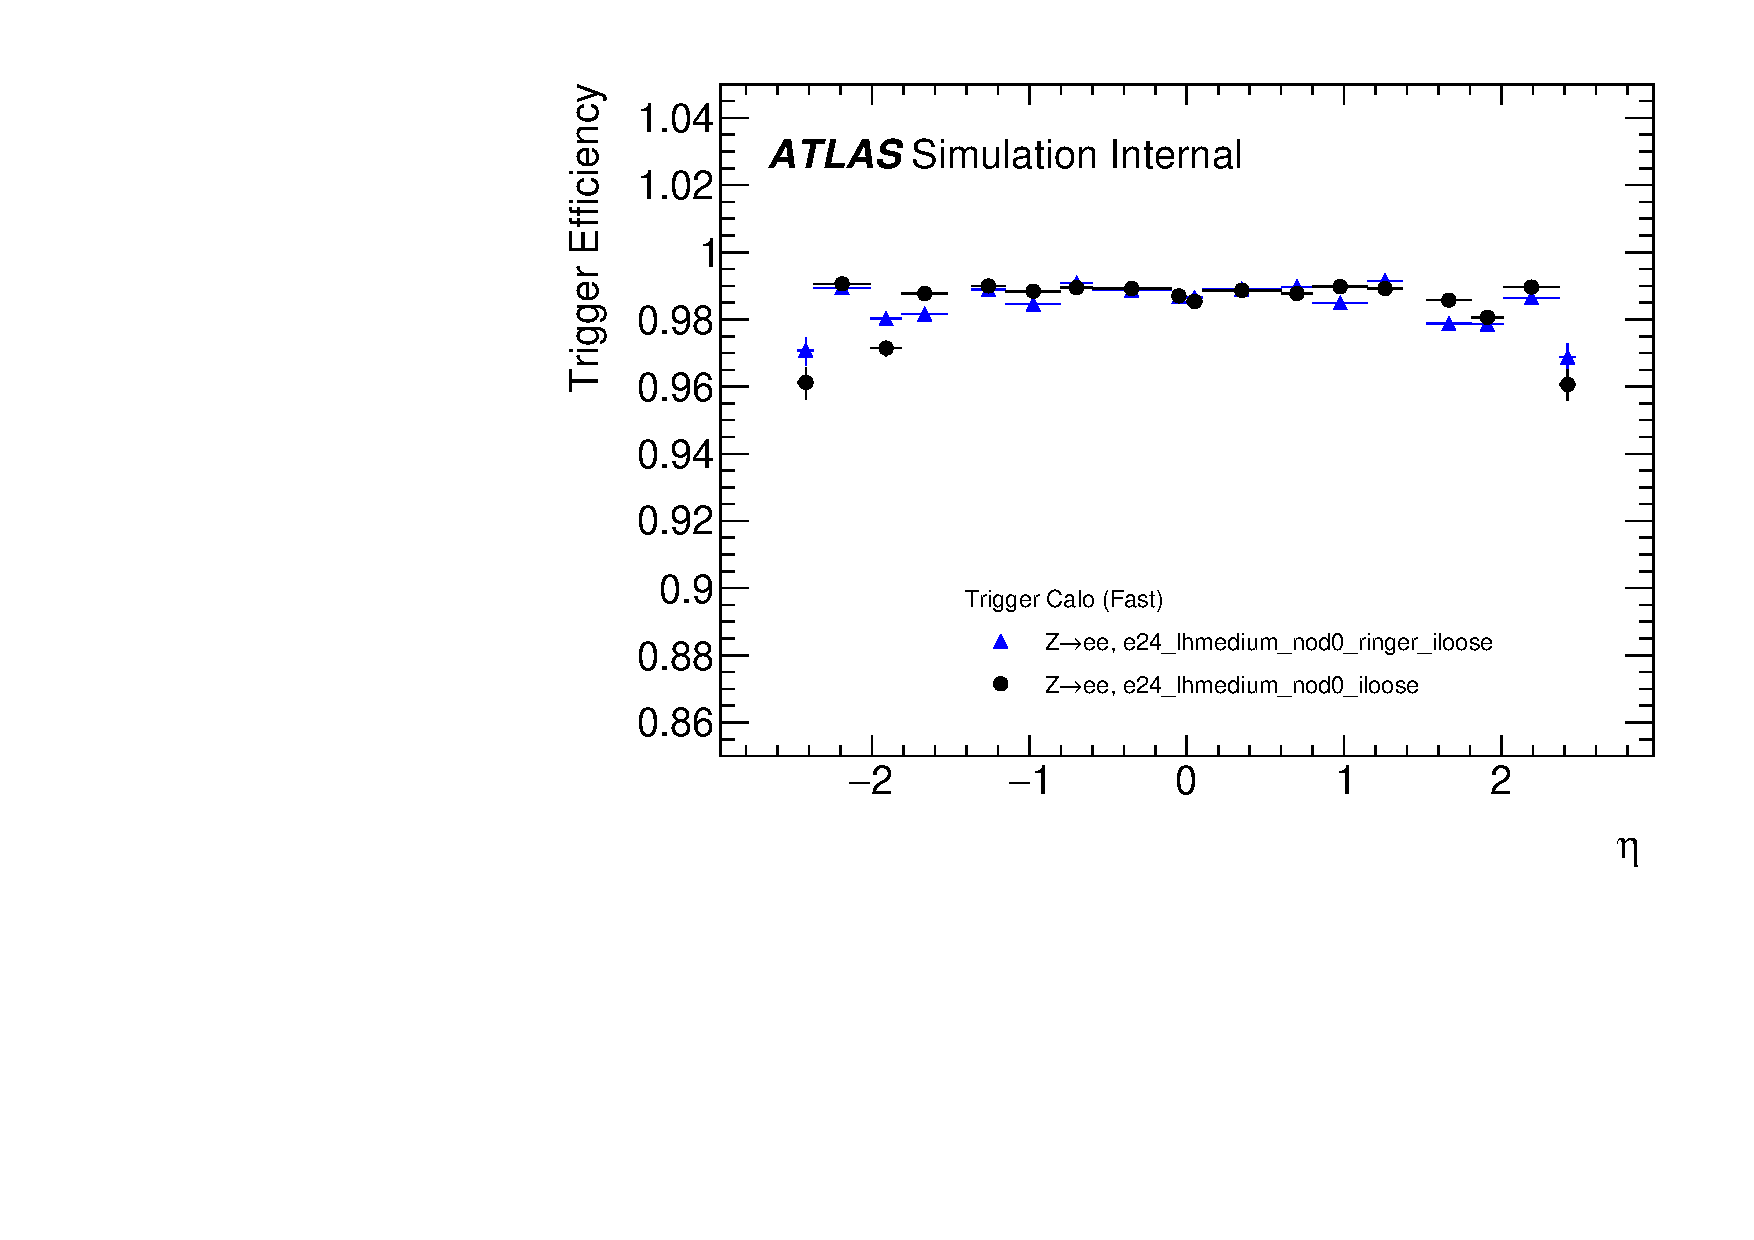
\includegraphics[width=0.6\textwidth]{figures/plots/plot_e24_lhmedium_hlt_eff_eta_tap.pdf}
\caption[As eficiências do método de \textit{tag-and-probe} em função de $\eta$.]{
As eficiências do método de \textit{tag-and-probe} em função de $\eta$ para cada uma das \textit{chains} listadas}
\label{fig:tap_eta}
\end{figure}

\newpage
Por fim, a Tabela~\ref{tab:tap_effs} mostra o resultado das eficiências das duas \textit{chains} para o método de \textit{tag-and-probe}.
Em conjunto, também foi adicionado os valores de falso alarme para os dois algoritmos utilizando todo o conjunto de dados de jatos. 
Como o valor de detecção do \textit{Neural Ringer} foi ajustado para obter valores de detecção, próximos do algoritmo de referência, então 
a comparação fica a critério da avaliação do falso alarme. Nesse caso, o \textit{Neural Ringer} obteve uma redução com um fator de $\sim2$ no conjunto de jatos.

\begin{table}[h] %\scriptsize
\centering
\begin{tabular}{ccc}
\hline
\hline
\textit{Fast Calorimeter step} & DET $T\&P$ {[}\%{]} & FA {[}\%{]} \\ \hline
e24\_lhmedium\_nod0\_iloose & \cellcolor[HTML]{FFFFFF}98.7221 & \cellcolor[HTML]{FFFFFF}{\color[HTML]{FE0000} 17.8995} \\ 
e24\_lhmedium\_nod0\_ringer\_iloose & \cellcolor[HTML]{FFFFFF}98.6269 & \cellcolor[HTML]{FFFFFF}{\color[HTML]{FE0000} 34.6124} \\ \hline  \hline
\end{tabular}
\caption[As eficiências de detecção pelo método de \textit{tag-and-probe} e falsos alarmes obtidos para as duas \textit{chains} listadas.]{
As eficiências de detecção pelo método de \textit{tag-and-probe} e falsos alarme obtidos para as duas \textit{chains} listadas.}
\label{tab:tap_effs}
\end{table}

A redução de praticamente a metade do falso alarme logo no primeiro algoritmo de hipótese do \textit{trigger} de alto nível
reduz pela metade o número de vezes de chamadas dos algoritmos de hipótese posteriores. Embora esses algoritmos
possuam a capacidade de eliminar os mesmos eventos rejeitados pelo \textit{Neural Ringer}, sua aplicação requer um tempo 
de latência maior e análises mais refinadas para inferir a mesma resposta que um simples classificador multi-camadas
apresentado como proposta para colaboração. Assim, a implementação de um sistema altamente eficiente combinado
com uma extração de características, no caso os anéis, mais completa resultou em uma classificação mais eficiente
que o algoritmo de referência utilizado como comparativo 






\chapter{Conclusões e Trabalhos Futuros}
\label{cap:conclusao}
\glsresetall

A informação de calorimetria é imprescindível para a operação do detector \acrshort{atlas}. Além da absorção
de grande parte das partículas produzidas pelas colisões geradas pelo \acrshort{lhc}, algumas não podem ser
detectadas corretamente sem o suporte dos calorímetros. Assim, esses sub-detectores acabam sendo
de extrema importância para as análises físicas.

Em geral, nesses tipos de experimento, onde para se observar os eventos de interesse são necessários
vários dias de colisão e cujo a massa de dados gerada é considerável, torna-se necessário um 
sistema de filtragem \textit{online}, uma vez que a separação dos eventos de interesse, no caso os elétrons provenientes
do decaimento do bóson Z, e das partículas hadrônicas, é extremamente necessário na identificação
destes canais.

Esse trabalho final de curso mostrou o uso da informação de calorimetria na tentativa de otimizar a banda
passante de aquisição de dados no sistema de filtragem \textit{online} do \acrshort{atlas}. Como elétrons
representam um grande interesse para a física, estudos detalhados foram feitos na tentativa de aumentar
a rejeição de eventos desinteressantes nesse canal.

Os resultados obtidos evidenciaram que uma nova forma de descrição
da informação de calorimetria nos detectores, combinada com a utilização de classificadores baseados em inteligência
artificial pode melhorar o desempenho do sistema de \textit{trigger}. Assim, a redução da taxa de falso 
alarme, logo na primeira etapa de discriminação do sistema, por um fator considerável, diminui, 
o número de vezes em que os algoritmos mais sofisticados sejam aplicados.

\section{Sistema de Filtragem de Calorimetria Rápida}

O uso da informação de calorimetria como sinal principal na identificação de partículas no \acrshort{atlas} foi estudada
utilizando uma comparação entre o atual algoritmo de extração de características de calorimetria baseado
na descrição do chuveiro da partícula, e o algoritmos de extração do \textit{Neural Ringer}, cuja informação de calorimetria
é mapeada em anéis concêntricos que descrevem a interação da partícula por toda a camada do calorímetro.

Neste ambiente, foi comparada a resposta dos algoritmos de hipótese para ambos os sistemas. Os estudos
utilizando simulação de Monte Carlo mostraram que o algoritmo \textit{Neural Ringer} possui uma alta rejeição
a RoIs não interessantes para o processo de interesse, no caso os jatos. Mantendo, neste caso, aproximadamente
a mesma probabilidade de detecção do algoritmo de referência.

O método de validação cruzada mostrou que a quantidade neurônios necessários é de 8 neurônios na
camada escondida. A rede de operação emulada dentro do ambiente de \textit{trigger} obteve uma eficiência de
\textit{tag-and-probe} parecida com a requerida pela colaboração no algoritmo do T2Calo, uma vez que essa rede
foi ajustada para ter a mesma eficiência. Assim, o principal ganho nesse caso foi a alta taxa de rejeição
a falso alarme, com um fator de redução de  $\approx2$ vezes quando comparada com a referência.

A proposta de utilização do índice máximo SP obtido na curva de operação da rede também obteve
resultados satisfatórios em termos de falso alarme. Nesse caso, o SP ajusta o limiar de decisão da rede
para se obter um balanço entre a probabilidade de detecção e o falso alarme.  Porém, em ambientes
de filtragem \textit{online} de eventos deve-se preservar a taxa de detecção, assim, apenas a rede
ajustada pela detecção da referência foi utilizada.


\section{Trabalhos Futuros}

Diversas estratégias estão sendo estudadas como forma de melhorar a eficiência do algoritmo de hipótese do
\textit{Neural Ringer}. Uma estrutura bastante comum implementada nos algoritmos de hipótese, atualmente, 
usados pela colaboração é a utilização de classificadores especialistas para cada região em $\eta$ do calorímetro e faixa de energia.
Em geral, esses algoritmos contam com pelo menos dezenas de classificadores que são selecionadas dependendo da posição e da energia
em $GeV$ do evento a ser testado. Os cortes também são ajustados dependendo da região e da energia. Assim, a próxima etapa do \textit{Neural Ringer}
é aplicar esse novo esquema de classificadores especialistas na etapa de hipotese.

Estudos preliminares também mostraram a possibilidade do \textit{Neural Ringer} substituir todos os algoritmos de hipótese do \textit{trigger} rápido mais 
a etapa de decisão da calorimetria de alta precisão. Assim, o  \textit{Neural Ringer} seria responsável por toda a cadeia de decisão baseada em calorimetria
no \textit{trigger} de alto nível. Por fim, como já mostrado em outros trabalhos, o pré-processamento também tem grande impacto nas eficiências dos 
classificadores. Assim, os próximos passos incluirão um pré-processamento mais sofisticado com técnicas de processamento de sinais para otimizar, ainda mais, 
a resposta do sistema de filtragem do \textit{Neural Ringer}.








%\input{conclusao}
\glsaddall

\cleardoublepage
\bibliographystyle{coppe}
\cleardoublepage \phantomsection \addcontentsline{toc}{chapter}{Referências Bibliográficas}
\bibliography{pf_bibliografia}
%\appendix
%\input{publicacoes}

\end{document}

